%----------
%   IMPORTANTE
%----------

% Si nunca has utilizado LaTeX es conveniente que aprendas una serie de conceptos básicos antes de utilizar esta plantilla. Te aconsejamos que leas previamente algún tutorial (puedes encontar muchos en Internet).

% Esta plantilla está basada en las recomendaciones de la guía "Trabajo fin de Máster: Escribir el TFM", que encontrarás en http://uc3m.libguides.com/TFM/escribir
% contiene recomendaciones de la Biblioteca basadas principalmente en estilos APA e IEEE, pero debes seguir siempre las orientaciones de tu Tutor de TFM y la normativa de TFM para tu titulación.

% Encontrarás un ejemplo de TFM realizado con esta misma plantilla en la carpeta "_ejemplo_TFM_2019". Consúltalo porque contiene ejemplos útiles para incorporar tablas, figuras, listados de código, bibliografía, etc.


%----------
%	CONFIGURACIÓN DEL DOCUMENTO
%----------

% Definimos las características del documento y añadimos una serie de paquetes (\usepackage{package}) que agregan funcionalidades a LaTeX.

\documentclass[12pt]{report} %fuente a 12pt

% MÁRGENES: 2,5 cm sup. e inf.; 3 cm izdo. y dcho.
\usepackage[
a4paper,
vmargin=2.5cm,
hmargin=3cm
]{geometry}

% INTERLINEADO: Estrecho (6 ptos./interlineado 1,15) o Moderado (6 ptos./interlineado 1,5)
\renewcommand{\baselinestretch}{1.15}
\parskip=6pt

% DEFINICIÓN DE COLORES para portada y listados de código
\usepackage[table]{xcolor}
\definecolor{azulUC3M}{RGB}{0,0,102}
\definecolor{gray97}{gray}{.97}
\definecolor{gray75}{gray}{.75}
\definecolor{gray45}{gray}{.45}

% Soporte para GENERAR PDF/A --es importante de cara a su inclusión en e-Archivo porque es el formato óptimo de preservación y a la generación de metadatos, tal y como se describe en http://uc3m.libguides.com/ld.php?content_id=31389625. En la carpeta incluímos el archivo plantilla_tfg_2017.xmpdata en el que puedes incluir los metadatos que se incorporarán al archivo PDF cuando lo compiles. Ese archivo debe llamarse igual que tu archivo .tex. Puedes ver un ejemplo en esta misma carpeta.
\usepackage[a-1b]{pdfx}

% ENLACES
\usepackage{hyperref}
\hypersetup{colorlinks=true,
	linkcolor=black, % enlaces a partes del documento (p.e. índice) en color negro
	urlcolor=blue} % enlaces a recursos fuera del documento en azul

% EXPRESIONES MATEMATICAS
\usepackage{amsmath,amssymb,amsfonts,amsthm}
\usepackage{subcaption}
\usepackage[super]{nth}
\usepackage{txfonts} 
\usepackage[T1]{fontenc}

\usepackage[utf8]{inputenc}

\usepackage[english]{babel} 
\usepackage[babel, english=american]{csquotes}
\AtBeginEnvironment{quote}{\small}

% diseño de PIE DE PÁGINA
\usepackage{fancyhdr}
\pagestyle{fancy}
\fancyhf{}
\renewcommand{\headrulewidth}{0pt}
\rfoot{\thepage}
\fancypagestyle{plain}{\pagestyle{fancy}}

% DISEÑO DE LOS TÍTULOS de las partes del trabajo (capítulos y epígrafes o subcapítulos)
\usepackage{titlesec}
\usepackage{titletoc}
\titleformat{\chapter}[block]
{\large\bfseries\filcenter}
{\thechapter.}
{5pt}
{\MakeUppercase}
{}
\titlespacing{\chapter}{0pt}{0pt}{*3}
\titlecontents{chapter}
[0pt]                                               
{}
{\contentsmargin{0pt}\thecontentslabel.\enspace\uppercase}
{\contentsmargin{0pt}\uppercase}                        
{\titlerule*[.7pc]{.}\contentspage}                 

\titleformat{\section}
{\bfseries}
{\thesection.}
{5pt}
{}
\titlecontents{section}
[5pt]                                               
{}
{\contentsmargin{0pt}\thecontentslabel.\enspace}
{\contentsmargin{0pt}}
{\titlerule*[.7pc]{.}\contentspage}

\titleformat{\subsection}
{\normalsize\bfseries}
{\thesubsection.}
{5pt}
{}
\titlecontents{subsection}
[10pt]                                               
{}
{\contentsmargin{0pt}                          
	\thecontentslabel.\enspace}
{\contentsmargin{0pt}}                        
{\titlerule*[.7pc]{.}\contentspage}  


% DISEÑO DE TABLAS. Puedes elegir entre el estilo para ingeniería o para ciencias sociales y humanidades. Por defecto, está activado el estilo de ingeniería. Si deseas utilizar el otro, comenta las líneas del diseño de ingeniería y descomenta las del diseño de ciencias sociales y humanidades
\usepackage{multirow} %permite combinar celdas 
\usepackage{caption} %para personalizar el título de tablas y figuras
\usepackage{floatrow} %utilizamos este paquete y sus macros \ttabbox y \ffigbox para alinear los nombres de tablas y figuras de acuerdo con el estilo definido. Para su uso ver archivo de ejemplo 
\usepackage{array} % con este paquete podemos definir en la siguiente línea un nuevo tipo de columna para tablas: ancho personalizado y contenido centrado
\newcolumntype{P}[1]{>{\centering\arraybackslash}p{#1}}
\DeclareCaptionFormat{upper}{#1#2#3\par}

% Diseño de tabla para ingeniería
\captionsetup[table]{
	format=upper,
	justification=centering,
	labelsep=period,
	width=.75\linewidth,
	labelfont=small,
	font=small,
}

%Diseño de tabla para ciencias sociales y humanidades
%\captionsetup[table]{
%	justification=raggedright,
%	labelsep=period,
%	labelfont=small,
%	singlelinecheck=false,
%	font={small,bf}
%}


% DISEÑO DE FIGURAS. Puedes elegir entre el estilo para ingeniería o para ciencias sociales y humanidades. Por defecto, está activado el estilo de ingeniería. Si deseas utilizar el otro, comenta las líneas del diseño de ingeniería y descomenta las del diseño de ciencias sociales y humanidades
\usepackage{graphicx}
\graphicspath{{figures/}} %ruta a la carpeta de imágenes

% Diseño de figuras para ingeniería
\captionsetup[figure]{
	format=hang,
	name=Fig.,
	singlelinecheck=off,
	labelsep=period,
	labelfont=small,
	font=small		
}

% Diseño de figuras para ciencias sociales y humanidades
%\captionsetup[figure]{
%	format=hang,
%	name=Figure,
%	singlelinecheck=off,
%	labelsep=period,
%	labelfont=small,
%	font=small		
%}


% NOTAS A PIE DE PÁGINA
\usepackage{chngcntr} %para numeración contínua de las notas al pie
\counterwithout{footnote}{chapter}

% LISTADOS DE CÓDIGO
% soporte y estilo para listados de código. Más información en https://es.wikibooks.org/wiki/Manual_de_LaTeX/Listados_de_código/Listados_con_listings
\usepackage{listings}

% definimos un estilo de listings
\lstdefinestyle{estilo}{ frame=Ltb,
	framerule=0pt,
	aboveskip=0.5cm,
	framextopmargin=3pt,
	framexbottommargin=3pt,
	framexleftmargin=0.4cm,
	framesep=0pt,
	rulesep=.4pt,
	backgroundcolor=\color{gray97},
	rulesepcolor=\color{black},
	%
	basicstyle=\ttfamily\footnotesize,
	keywordstyle=\bfseries,
	stringstyle=\ttfamily,
	showstringspaces = false,
	comment=[l]{\#},
	commentstyle=\color{gray45},     
	%
	numbers=left,
	numbersep=15pt,
	numberstyle=\tiny,
	numberfirstline = false,
	breaklines=true,
	xleftmargin=\parindent
}

\captionsetup[lstlisting]{font=small, labelsep=period}
% fijamos el estilo a utilizar 
\lstset{style=estilo}
\renewcommand{\lstlistingname}{\uppercase{Código}}


%BIBLIOGRAFÍA - PUEDES ELEGIR ENTRE ESTILO IEEE O APA. POR DEFECTO ESTÁ CONFIGURADO IEEE. SI DESEAS USAR APA, COMENTA LAS LÍNEA DE IEEE Y DESCOMENTA LAS DE APA. Si haces cambios en la configuración de la bibliografía y no obtienes los resultados esperados, es recomendable limpiar los archivos auxiliares y volver a compilar en este orden: COMPILAR-BIBLIOGRAFIA-COMPILAR
% Tienes más información sobre cómo generar bibliografía en http://tex.stackexchange.com/questions/154751/biblatex-with-biber-configuring-my-editor-to-avoid-undefined-citations , https://es.sharelatex.com/learn/Bibliography_management_in_LaTeX y en http://www.ctan.org/tex-archive/macros/latex/exptl/biblatex-contrib
% También te recomendamos consultar la guía temática de la Biblioteca sobre citas bibliográficas: http://uc3m.libguides.com/guias_tematicas/citas_bibliograficas/inicio

% CONFIGURACIÓN PARA LA BIBLIOGRAFÍA IEEE
\usepackage[backend=biber, style=ieee, isbn=false,sortcites, maxbibnames=5, minbibnames=1]{biblatex} % Configuración para el estilo de citas de IEEE, recomendado para el área de ingeniería. "maxbibnames" indica que a partir de 5 autores trunque la lista el primero (minbibnames) y añada "et al." tal y como se utiliza en el estilo IEEE.

%CONFIGURACIÓN PARA LA BIBLIOGRAFÍA APA
%\usepackage[style=apa, backend=biber, natbib=true, hyperref=true, uniquelist=false, sortcites]{biblatex}
%\DeclareLanguageMapping{spanish}{spanish-apa}

\addbibresource{bibliography/bibliography.bib} % llama al archivo bibliografia.bib que utilizamos de ejemplo


%-------------
%	DOCUMENTO
%-------------

\begin{document}
\pagenumbering{roman} % Se utilizan cifras romanas en la numeración de las páginas previas al cuerpo del trabajo
	
%----------
%	PORTADA
%----------	
\begin{titlepage}
	\begin{sffamily}
	\color{azulUC3M}
	\begin{center}
		\begin{figure}[H] %incluimos el logotipo de la Universidad
			\makebox[\textwidth][c]{
\includegraphics[width=16cm]{Portada_Logo.png}}
		\end{figure}
		\vspace{1cm}
		\begin{Large}
			Master in Telecommunication Engineering\\			
			2018-2020\\
			\vspace{1cm}		
			\textsl{Master Thesis}
			\bigskip
			
		\end{Large}
		 	{\Huge ``Embedded solution for person identification and tracking with a robot''}\\
		 	\vspace*{0.5cm}
	 		\rule{10.5cm}{0.1mm}\\
			\vspace*{0.9cm}
			{\LARGE Ignacio Condés Menchén}\\ 
			\vspace*{1cm}
		\begin{Large}
			Fernando Díaz de María\\
			Eduardo Perdices García\\
			Leganés, 2020\\
		\end{Large}
	\end{center}
	
	\vfill
	\color{black}
	\begin{footnotesize}
%	\noindent\fbox{
%	\begin{minipage}{\textwidth}
%		\textbf{AVOID PLAGIARISM}\\
%		The University uses the \textbf{Turnitin Feedback Studio} program within the Aula Global for the delivery of student work. This program compares the originality of the work delivered by each student with millions of electronic resources and detects those parts of the text that are copied and pasted. Plagiarizing in a TFM is considered a \textbf{Serious Misconduct}, and may result in permanent expulsion from the University.
%	\end{minipage}	
%	}
%	\vspace*{.5cm}\\	
	\noindent
\includegraphics[width=4.2cm]{creativecommons.png}\\
%	\emph{[Include this code in case you want your Master Thesis published in Open Access University Repository]}\\
	This work is licensed under Creative Commons \textbf{Attribution – Non Commercial – Non Derivatives}

	\end{footnotesize}
	\end{sffamily}
\end{titlepage}

\newpage %página en blanco o de cortesía
\thispagestyle{empty}
\mbox{}

\pretolerance=10000 % evitar cortes de palabras
%----------
%	RESUMEN Y PALABRAS CLAVE
%----------
\renewcommand\abstractname{\large\uppercase{Summary}}
\begin{abstract}
\thispagestyle{plain}
\setcounter{page}{3}
	% ESCRIBIR EL RESUMEN AQUÍ
	
	This project describes the development process of an embedded system capable of performing a reactive following of a person. It makes use of convolutional neural networks and probabilistic tracking for processing the perception acquired by a RGBD camera. This input is processed in a NVIDIA Jetson TX2, an embedded SoM (\textit{System-on-Module}). This device is capable of performing computationally demanding tasks onboard, coping with the complexity required to run a robust tracking and following algorithm. The full design is implemented on a robotic mobile base, which receives velocity commands from the board, intended to move towards the desired person.
	
	\textbf{Keywords:}
	% Escribir las palabras clave aquí
	deep learning, robotics, person following, rgbd
	
	\vfill
\end{abstract}
	\newpage %página en blanco o de cortesía
	\thispagestyle{empty}
	\mbox{}


%----------
%	DEDICATORIA
%----------	


\setcounter{page}{5}
\newgeometry{voffset=-2.8cm,bottom=-0.6cm,textwidth=15cm}
\chapter*{Dedication}
La escritura de estas palabras cierra este capítulo en mi vida académica. Muchos meses de continua lucha me han traído, madrugada de estudio tras madrugada de estudio, hasta el final del camino, en el que puedo dar por terminada la consecución de este máster. Tengo que agradecer a muchas personas por todo el apoyo, material y emocional, que me han brindado durante este tiempo.\\

Para empezar, a mis queridos compañeros, colegas y amigos del máster. Cuando todos llegamos aquí desde los rincones más diversos de España, la dificultad, y la calidad y calidez del grupo fomentaron que enseguida fuéramos una piña inquebrantable. Y salimos adelante pese a enfrentarnos a más momentos duros de lo que al principio estimábamos. Con humor, con fuerza y sobre todo con ese saber hacer que finalmente nos ha hecho superar esta etapa tan exigente pero a la vez tan satisfactoria: lo hemos conseguido.\\

Además, les debo un profundo agradecimiento a mis tutores, Eduardo Perdices y Fernando Díaz, y sobre todo a José María Cañas, por cuánto se han volcado en este proyecto conmigo, en especial en esta última etapa de escritura para ayudarme a mantener el rigor y la calidad necesarios en este proyecto. Gracias por vuestra paciencia e involucración.\\

También, por supuesto, a mis compañeros y amigos de AFC Ingenieros, que me han aguantado, ayudado y animado con este proyecto cada vez que me veían entrar al laboratorio con mi famoso robot y un puñado de cables para soldar una y otra vez, ``que esta era la buena''. Por otro lado, gracias a AFC Ingenieros como tal, por la enorme flexibilidad que me ha permitido compatibilizar mi empleo con el seguimiento regular del máster. Sin esa confianza y empatía, me habría sido imposible completarlo.\\

Asimismo, quiero destacar  los ánimos y el cariño que me ha infundido la gente que me soporta cada día. Quiero agradecérselo a mis mejores amigos, Jose y Jorge, a mi banda (qué mal tocamos ¡pero qué bien lo pasamos!), a toda mi familia y en especial a mi abuela, que ha animado durante tantos meses a un nieto pegado a un ordenador, siempre con demasiadas cosas pendientes por terminar.\\

Finalmente, y al igual que en entregas anteriores, sigo sin tener palabras para condensar el infinito cariño, comprensión, desahogo y empatía que mi pareja ha tenido conmigo. Almudena, aunque sé que te mueres de vergüenza por aparecer aquí, quiero dejar constancia de la pieza fundamental que eres en el rompecabezas de mi vida, de que este proyecto ha salido adelante respaldado por el gran aguante y entereza que has tenido las innumerables veces que nuestra relación se ha visto reducida a un eterno ``hoy no puedo, tengo que avanzar con el TFM''. Un millón de gracias a ti y a tu familia por haber sido mi fuente de fuerzas tantas veces sin ninguna reserva.

\restoregeometry
	\vfill
	
	\newpage %página en blanco o de cortesía
	\thispagestyle{empty}
	\mbox{}
	

%----------
%	ÍNDICES
%----------

%--
%Índice general
%-
\tableofcontents
\thispagestyle{fancy}

\newpage %página en blanco o de cortesía
\thispagestyle{empty}
\mbox{}

%--
%Índice de figuras. Si no se incluyen, comenta las líneas siguientes
%-
\listoffigures
\thispagestyle{fancy}

\newpage  % página en blanco o de cortesía
\thispagestyle{empty}
\mbox{}

%--
%Índice de tablas. Si no se incluyen, comenta las líneas siguientes
%-
\listoftables
\thispagestyle{fancy}

\newpage %página en blanco o de cortesía
\thispagestyle{empty}
\mbox{}

%----------
%	TRABAJO
%----------	
\clearpage
\pagenumbering{arabic} % numeración con números arábigos para el resto de la publicación	

\chapter{Introduction}
\section{Motivation}
	This work is focused on exploring the synergy between two science fields, which are outstanding nowadays: \textit{robotics} and \textit{deep learning}. These are combined for obtaining a robust system capable of following a certain person navigating towards it on a reactive behavioral. This behavioral is composed of two main components: the \textit{perception block}, responsible of processing the images from an RGB-D sensor placed on the system, and the \textit{actuation block}, which moves the robotic base accordingly to the relative position of the person to be followed.\\
	
	The original idea was proposed on \cite{tfg}, where a neural following system was developed to be run in a standard laptop into which the camera and the robot were plugged. In the following dissertation, we will revisit this work and describe the points of interest which have allowed to enhance the previous version of this work.\\
	
	The key aspects of this project can be brought in as follows:
	\begin{description}
		\item[Embedded solution] the system is mounted on a battery-powered robot, on a \textit{mobile base} form factor. This robot features a high-performance GPU embedded on a System-on-Module. Thus, this ensemble can work on its own, without requiring an external computer to perform the inferences or running algorithms in parallel. A remote monitoring of the behavioral is available as well, but it is not required for the system to work.

		\item[Person identification] the proposed system runs 3 neural networks. These networks perform inferences over the images perceived by the RGB-D sensor, which is attached to the system as the \textit{point-of-view} of the robot. The inferences are devoted to detect the different persons present in the scene, as well as to distinguish them by means of an distinguishing feature: their face.

		\item[Tracking] the full system includes a probabilistic tracker, based on dynamic modeling. This leverages the \textit{trajectories} followed by the persons while they wander on the visual field of the robot, as well as the relative distance to the person, obtained by the depth sensor included in the camera. As a result, we can have a gain on the robustness of the system, compared to a version governed exclusively by the neural inferences, which are sensitive to visual occlusions. Trusting just on these inferences could easily result on an unsteady behavioral. However, this can be avoided introducing the probabilistic modeling, as it will be explained later.
	\end{description}
	
	%	Este proyecto describe el proceso de desarrollo del sistema enunciado en el título, que condensa los puntos clave que conforman la novedad con la que justificamos el mismo:
	%- Embedded, ya que está compuesto de un robot alimentado por una batería, que soporta una placa portátil de desarrollo. Esta placa implementa algoritmos de manera totalmente local, ofreciendo una monitorización inalámbrica del funcionamiento del sistema.
	%- Person identification, combinamos de manera secuencial 3 redes neuronales que realizan inferencias sobre las imágenes percibidas por la cámara RGB-D incorporada en el robot. Este sistema combinado permite detectar a las diferentes personas presentes en la escena, así como discernir entre estas mediante un signo de identidad como es la cara.
	%- Tracking, ya que incorpora un seguimiento probabilístico basado en sistemas dinámicos. Esto se aprovecha de las trayectorias que mantienen las personas al moverse por el campo visual del robot, así como de la distancia relativa del robot a cada una de estas, gracias al sensor óptico de profundidad incorporado. Este sistema provee una robustez extra del sistema frente a posibles pérdidas totales o parciales de la persona, ante las cuales las inferencias neuronales no serían suficientes para mantener un control estable sobre el robot.
	
	
\section{State of the art}
\label{sec:1_sota}
	As it was previously introduced, this work is performed to explore the synergies on robotics and deep learning. In this section, the current approaches and tools will be studied in order to outline a general framework where this work can be placed.\\
	
	The problem to be addressed is to \textit{get a robot to follow a person}. This problem can be split into several steps, where different approaches have been previously developed. The steps will be covered in the following subsections.
	
\subsection{Person detection}
Last decades have come linked to strong advances in the computer vision field. This has vastly reduced the production prices of digital cameras and high-resolution sensors, which have come into the consumer market segment: nowadays, everybody carries at least 2 cameras in their mobile phone. This, besides an increase in the hardware performance has resulted in a strong impulse into computer vision research. There are many application possibilities using cameras, however the \textit{person detection} challenge is a recurrent one.\\

\begin{figure}[h]
	\centering
	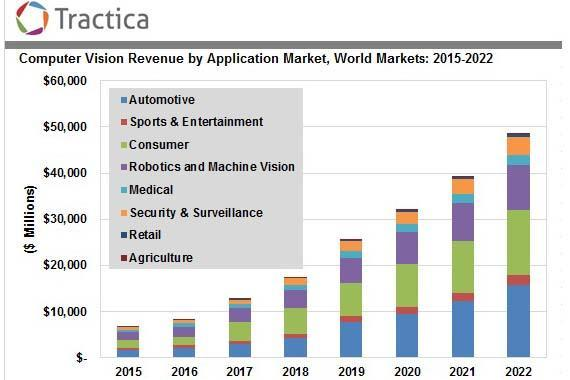
\includegraphics[width=10cm]{cv_forecast_2022}
	\caption{Computer Vision revenues in the last year, and forecast for 2022 (source: \cite{cv_forecast}).}
	\label{fig:1_cv_forecast}
\end{figure}

One of the mostly used approaches is commonly called the \textit{Viola-Jones} detector \cite{violajones}. This algorithm relies on a \textit{rigid body model}, which fits a specific shape. On a grayscale image, this shape can be typically distinguished by means of the pixel intensity levels. A spatial filters called \textit{Haar features} (\autoref{fig:1_haarfeats}) are introduced: these are used across the image looking for the intensity pattern for each mask, which should resemble a part of the rigid body. As this presents a weak decision by itself, several filters (previously chosen in a training process) are combined on a \textit{boosted cascade}. A person is detected if the weighted combination of several filters are triggered inside a certain area, which is decided to potentially contain a person \cite{diapos_cv_clasif}.

\begin{figure}[h]
	\centering
	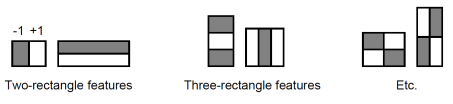
\includegraphics[width=0.7\linewidth]{haar_feats}
	\caption{Haar features: some examples \cite{diapos_cv_clasif}.}
	\label{fig:1_haarfeats}
\end{figure}

\begin{figure}[h]
	\centering
	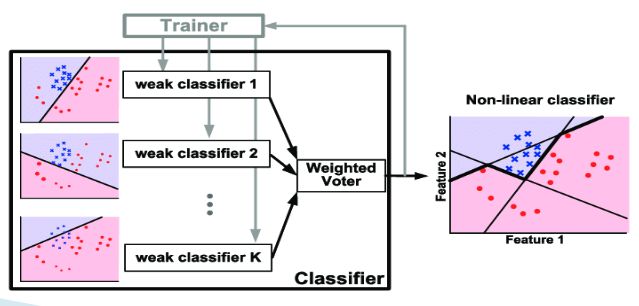
\includegraphics[width=0.7\linewidth]{boosted_cascade}
	\caption{Boosted weak classifiers \cite{diapos_cv_clasif}.}
	\label{fig:1_violajones_boost}
\end{figure}

Although this system was originally developed to detect faces, the rigid body model allows a generalization powerful enough to extend this to another object classes, \textit{person} among these. The open-source standard image processing library, OpenCV, includes pre-trained models\footnote{\url{https://github.com/opencv/opencv/blob/master/data/haarcascades}}, which can be directly used in their Viola-Jones implementation. Scale invariance can be achieved evaluating the image at multiple scales on runtime.


Another common approach nowadays for person detection is based on HoG (\textit{Histograms of Gradients}) \cite{hog_detection}. This method computes local features by means of the intensity gradients across the image, and quantizes them using their angle (creating a histogram for the oriented gradients for that pixel), as it can be seen on \autoref{fig:1_hog_sift}.\\


\begin{figure}[h]
	\centering
	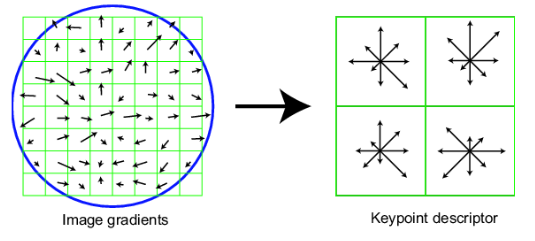
\includegraphics[width=0.7\linewidth]{hog_sift}
	\caption{Example of a HoG, quantized to 8 directions \cite{diapos_cv_features}.}
	\label{fig:1_hog_sift}
\end{figure}



These gradients are collected in $64 \times 128$ windows, and treated as features from which a linear SVM (\textit{Support Vector Machine}) is trained in order to classify a region as \textit{person/non-person}. \autoref{fig:1_hog_avg} shows the average gradient patch for a person (the direction of each gradient is not shown). A visual inspection immediately resembles the shape of a person standing up. Thus, this detector will yield the best performance when the person to be detected stands in that specific pose.

\begin{figure}[h]
	\centering
	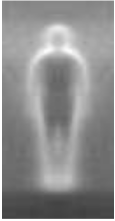
\includegraphics[width=3cm]{hog_avg}
	\caption{Average gradient for person detection on \cite{hog_detection}.}
	\label{fig:1_hog_avg}
\end{figure}

These methods, among several more approaches, have been the state-of-the-art techniques: the cornerstone are the image gradients, which can be computed with a high efficiency and present decent performance. However, their main drawback is the \textit{generalization} capability, as a successful detection is highly dependent on the person pose. However, in the latest advances, the detection frameworks have moved towards the spreading framework: \textit{deep learning}, especially the most salient tools on image processing: CNNs (\textit{convolutional neural networks}). The first steps on this field \cite{rcnn} required for a previous step on the image called \textit{region proposal}. This step is devoted to find potential regions on the image to contain an object. This way, the challenge was to label these region according to the objects contained inside, reducing the problem to a classification task. However, the process to find these undetermined regions and iterate over them makes the process too slow for real-time requirements, which are explicitly contained in our objectives. Care has been put in posterior works \cite{fastrcnn} \cite{spp} to reduce this computation time. However, this reduction in time brings about a reduction in precision as well.\\


On the other hand, one of the most remarkable architectures is SSD (\textit{Single-Shot Multibox Detector}) \cite{ssd}. The main benefit from this architecture is the fact that it embeds all the required computations in a single neural network, reducing the complexity compared to other approaches requiring external region proposals, as it was depicted above. This greatly reduces the computational time when the network has to evaluate an image. As it was depicted in \cite{tfg}, the architecture is split into stages:\\

% ============================================================================

\begin{description}
	
	\item[Reshape] the posterior stages evaluate the image on a fixed tensor size of $n \times 300 \times 300 \times 3$ (being $n$ the size of the input batch). Other image sizes might be used, however this one offers a good trade-off between score and computational load.
	
	\item [Base network] this first group of layers are reused from a typical image classification model, such as VGG-16 \cite{vgg16}. The first layer from this architecture are utilized in this design, truncated before the first classification layer. This way, the network can leverage the \textit{feature maps} from the classification network, in order to find objects inside the input image. At the output of this network, several convolutional layers are appended, decreasing in size. This has the objective of predict detections at multiple scales. One thing to mention at this point is that the base network can be a different one rather than VGG-16, such as a MobileNet \cite{mobilenet}, which is highly optimized for running on low specifications devices. This is interesting as our embedded system will be limited in computing power, thus it will be revisited in future sections.
	
	\item[Box predictors] later, for each extracted set, a dedicated operation is performed, generating a small set (typically 3 or 4) fixed-size \textit{anchors}, with varying aspect ratios for each cell on a grid over the activation map (\autoref{fig:5_ssd_generated_boxes}). As these maps have different sizes, this aims to detect  objects in different scales. The anchors are then convolved with small filters (one per depth channel), which output \emph{softmaxed confidence values for each known class}, and \emph{offsets/adjustments for the generated bounding box}. So, for each detected object (on that scale), we know the score for each class and its estimated position inside the feature map (hence, in the image as well).
	
	\item \emph{Postprocessor}: as several detections might be triggered in the same area for different classes and scales, a \textit{Non-Maximum-Supression} operation is performed at the output of the network to retain the boxes with a larger area.
\end{description}
	\begin{figure}[h]
	\centering
	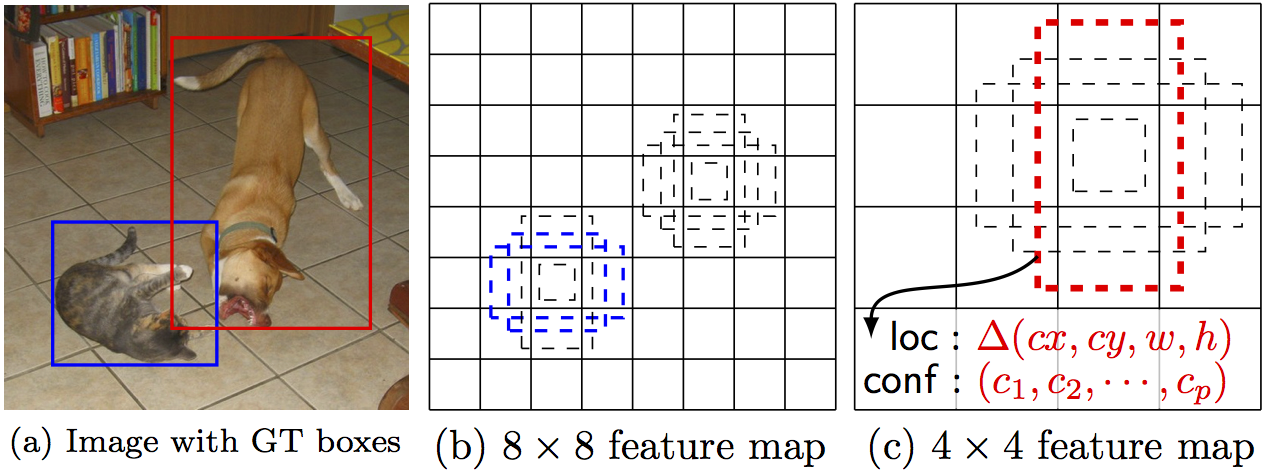
\includegraphics[width=0.7\linewidth]{ssd_generated_boxes}
	\caption{A set of boxes are generated centered on each point of every feature map \cite{ssd}.}
	\label{fig:5_ssd_generated_boxes}
\end{figure}


Another interesting approach on the neural networks field is the YOLO (\textit{You Only Look Once}) system \cite{yolov1}, which has been iteratively revised in two occasions so far \cite{yolov2} \cite{yolov3}.

The latest implementation, YOLOv3 \cite{yolov3} features residual networks \cite{resnets}, which tackle the problem of \textit{vanishing gradients} when the networks become deeper. The stacking of several layers results on gradients diminishing its value up to a point the precision mode of the machine is not able to handle. The gradients are canceled, burdening the training process, as the first layers parameters take a substantially higher time to converge. The residual networks added in this revision of the design add shortcut connections across the layers, centering the backpropagation gradients on 1. As the publication says \cite{yolov3}, the combination of these residual layers and convolutional ones allows to train much deeper architectures, capable of yielding a higher generalization. As in the SSD detectors, the YOLO architecture performs multi-scale detections, using 3 scales for splitting the feature maps into cell grids. On each of these cells, 3 anchor bounding boxes are fit. These anchors are selected by running the k-means algorithm on the COCO datasets selecting 9 clusters (3 anchor shapes $\times$ 3 scales). This aims to a better generalization as well, as in the R-CNN \cite{rcnn} and the SSD \cite{ssd} the anchor shapes are hand-picked.\\

For each (anchor, cell, scale) combination, this network predicts:

\begin{itemize}
	\item The coordinates of the object inside the anchor. Details can be visualized on \autoref{fig:1_yolo_output}.
	
	\item \textit{objectness} score, which is computed by means of a logistic regression in order to determine the probability of overlap with a ground truth bounding box more than any other prior anchor.
	
	\item 80 scores, as the original implementation is trained in the COCO dataset, which contains 80 classes. These classes might be overlapping (e.g. ``woman" and ``person"). Thus, these scores are computed by independent logistic classifiers and are not passed through a \textit{softmax} operation.
\end{itemize}


\begin{figure}[h]
	\centering
	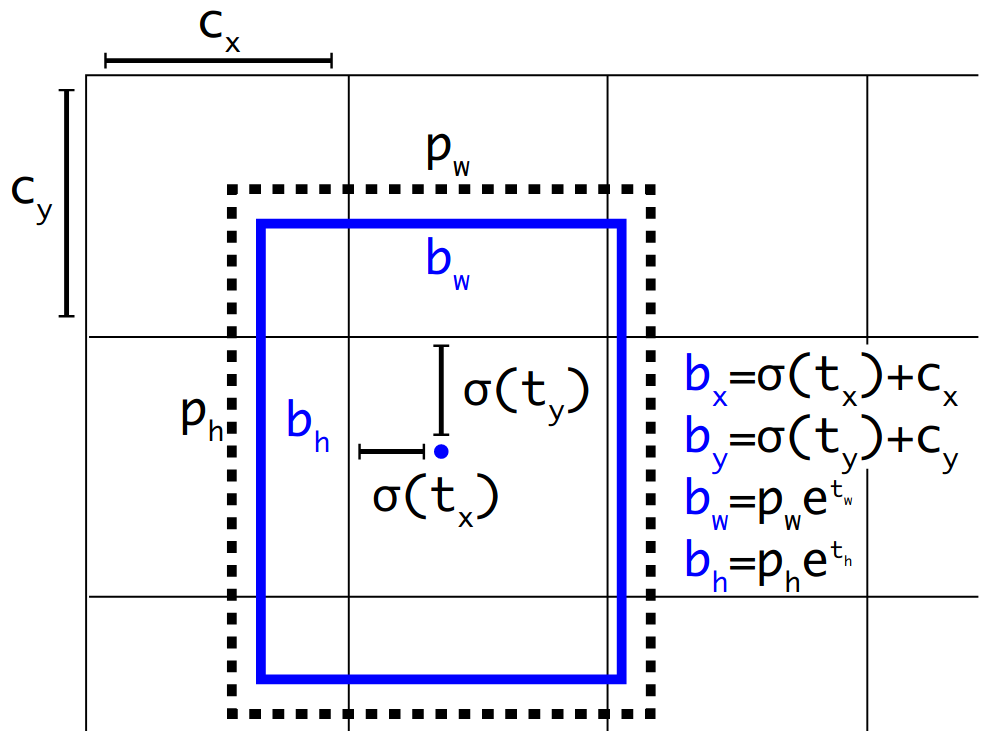
\includegraphics[width=0.5\linewidth]{yolo_outputs}
	\caption{Output on YOLO for each anchor and cell. The dashed line represents the prior anchor, while the blue line represents the detection which corrects that anchor.}
	\label{fig:1_yolo_output}
\end{figure}

\subsection{Person identification}
On a controlled environment, where the only present person is the one to be followed, a person detection system could be enough for following purposes. However, in a normal scenario, there might be several people inside the field of vision of the robot. This problem can be approached by means of adistinguishing feature of the person of interest, provided beforehand. One example is \cite{color_id}, which computes the color distribution of the person of interest, and later compares this distribution with the ones belonging to the different persons using the Bhattacharyya coefficient, which is designed to measure the similarity between the color histograms of the reference person and the detected one. However, this system can be deceived replicating the color distribution of the person of interest: wearing similar clothes helps to reduce the distance between the histogram, leaving a chance to confound another person with the one to follow.\\

A more robust approach is to use the \textit{face} of the person as the distinguishing feature, as its uniqueness makes it a good reference to identify the detected person. Several approaches \cite{dlib_review} extract facial \textit{landmarks} from the morphology of a given face, and use them to classify the face, comparing it against a set of known faces and predicting the identity based on the distance to each known face. Some open-source libraries such as \texttt{dlib} and \texttt{OpenCV} provide the algorithms to perform these processes.\\

\begin{figure}[h]
	\centering
	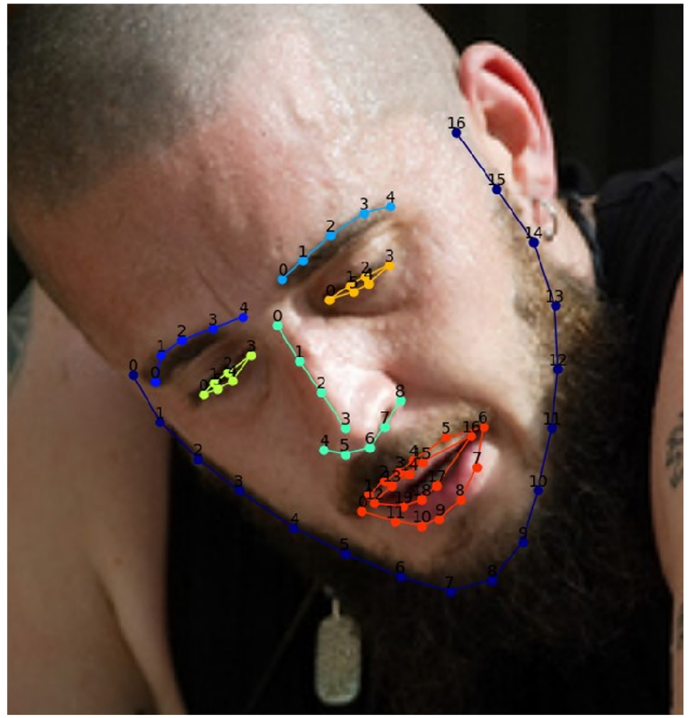
\includegraphics[width=0.6\linewidth]{dlib_landmarks}
	\caption{Facial landmarks are dependent of the face shape and morphology (image from \cite{dlib_review}).}
	\label{fig:1_dlib_landmarks}
\end{figure}


The intuition behind these methods are to \textit{project} the image of the face into a lower dimensional space, which allows to extract significant features from each face. These features have to be consistent for the same face across different pose and lighting conditions (\autoref{fig:1_faces_poses}). An useful transformation when a dimensionality reduction is pursued is PCA (\textit{Principal Component Analysis}), a linear transformation that can be implemented to deal with the face recognition problem \cite{face_pca}.

\begin{figure}[h]
	\centering
	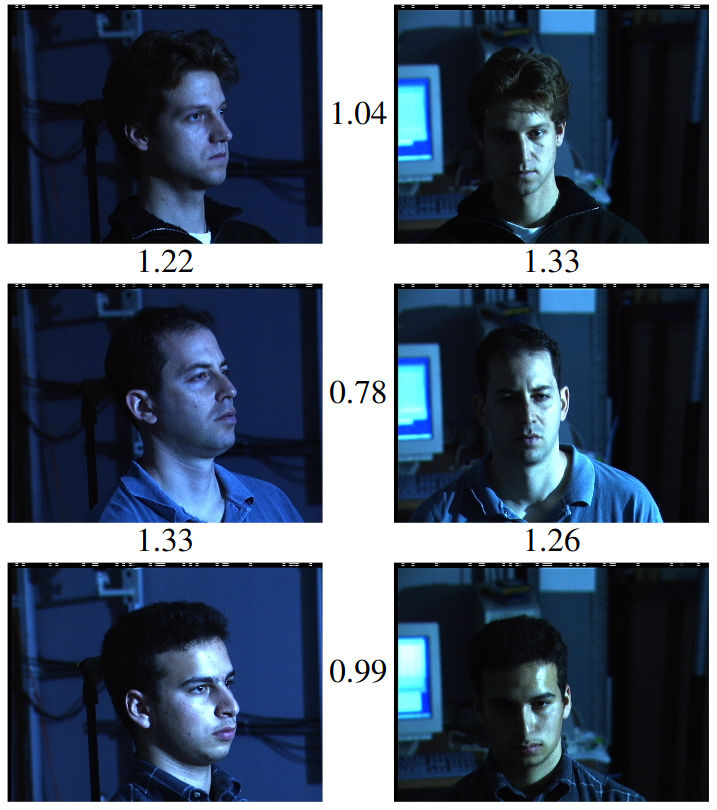
\includegraphics[width=0.5\linewidth]{face_poses}
	\caption{Examples of poses and light conditions across which the face projections are desired to be consistent for the same person (image from \cite{facenet}).}
	\label{fig:1_faces_poses}
\end{figure}


However, once again neural networks can be leveraged in order to achieve this and more: as the PCA is a linear operation, it could be learned by a single layer neural network. Thus, the introduction of deep networks can yield interesting results. The most relevant approach so far uses deep convolutional networks for performing this process \cite{facenet}, implementing an architecture called \textit{FaceNet}, which is partially based on the Inception \cite{inception} module, designed by Google researchers in order to greatly reduce the number of parameters in a neural network. What this network computes is called an \textit{embedding}, a projection of the input face image into a point in a 128-dimensional hypersphere. This allows to translate the identification into linear algebra terms, such as \textit{distance} between two faces, clustering and applying unsupervised algorithms in order to determine the identity of a trivial face, among a collection of known regions. These networks can be trained using a loss function  called \textit{triplet loss}, inspired by the work in \cite{lmnn_loss}. Given a training sample (\textit{anchor}), a \textit{positive} example (same class than the anchor) and a \textit{negative} example (different class than the anchor) are chosen, and the network is tuned to maximize the \textit{anchor-negative} embeddings distance, and minimize at the same time the \textit{anchor-positive} one (\autoref{fig:1_facenet_triplet_loss}).

\begin{figure}[h]
	\centering
	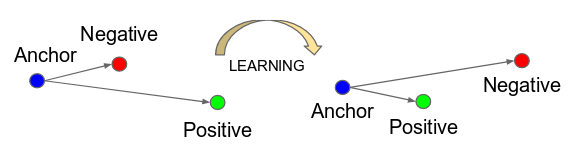
\includegraphics[width=0.7\linewidth]{facenet_triplet_loss}
	\caption{Triplet loss training. It minimizes the distance between an \emph{anchor} (current example) and a \emph{positive}, both of which have the same identity, and maximizes the distance between the \emph{anchor} and a \emph{negative} of a different identity (from \cite{facenet}).}
	\label{fig:1_facenet_triplet_loss}
\end{figure}


One thing to mention about the algorithms described above is that they perform the operations on the image of a face. Thus, a face detection system is required for previously cropping the face of the person to be identified. Once again, a neural approach can be reduced to an \textit{object detection} problem (detecting the class \textit{face}, in this case). One interesting approach using this technique is \textit{faced} \cite{faced}. This is a custom small ensemble of two neural networks, responsible to detect faces and correct the bounding boxes found. The main objective of the system is \textit{speed}, so the main detector architecture is based in YOLO \cite{yolov1}, and the second correction stage raises the precision achieved by the detector.

\begin{figure}[h]
	\centering
	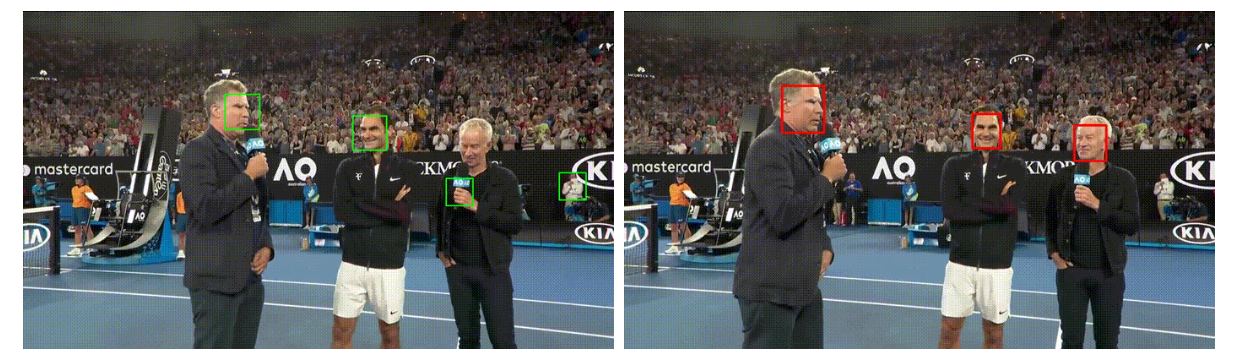
\includegraphics[width=0.8\linewidth]{faced_vs_haar}
	\caption{Classical Haar based face detector \cite{violajones} (left) vs. \textit{faced} (right). Image from \cite{faced}.}
	\label{fig:1_faced_vs_haar}
\end{figure}


%\subsection{Person tracking}

\subsection{Embedded deployment}
One of the requirements of this work is to be integrated in an autonomous system. This imposes a power limitation on the algorithms to be deployed. Generally, the robotic systems are deployed using laptops connected to robots, at it was done in \cite{tfg}.

\begin{figure}[h]
	\centering
	\begin{subfigure}[h]{0.4\linewidth}
		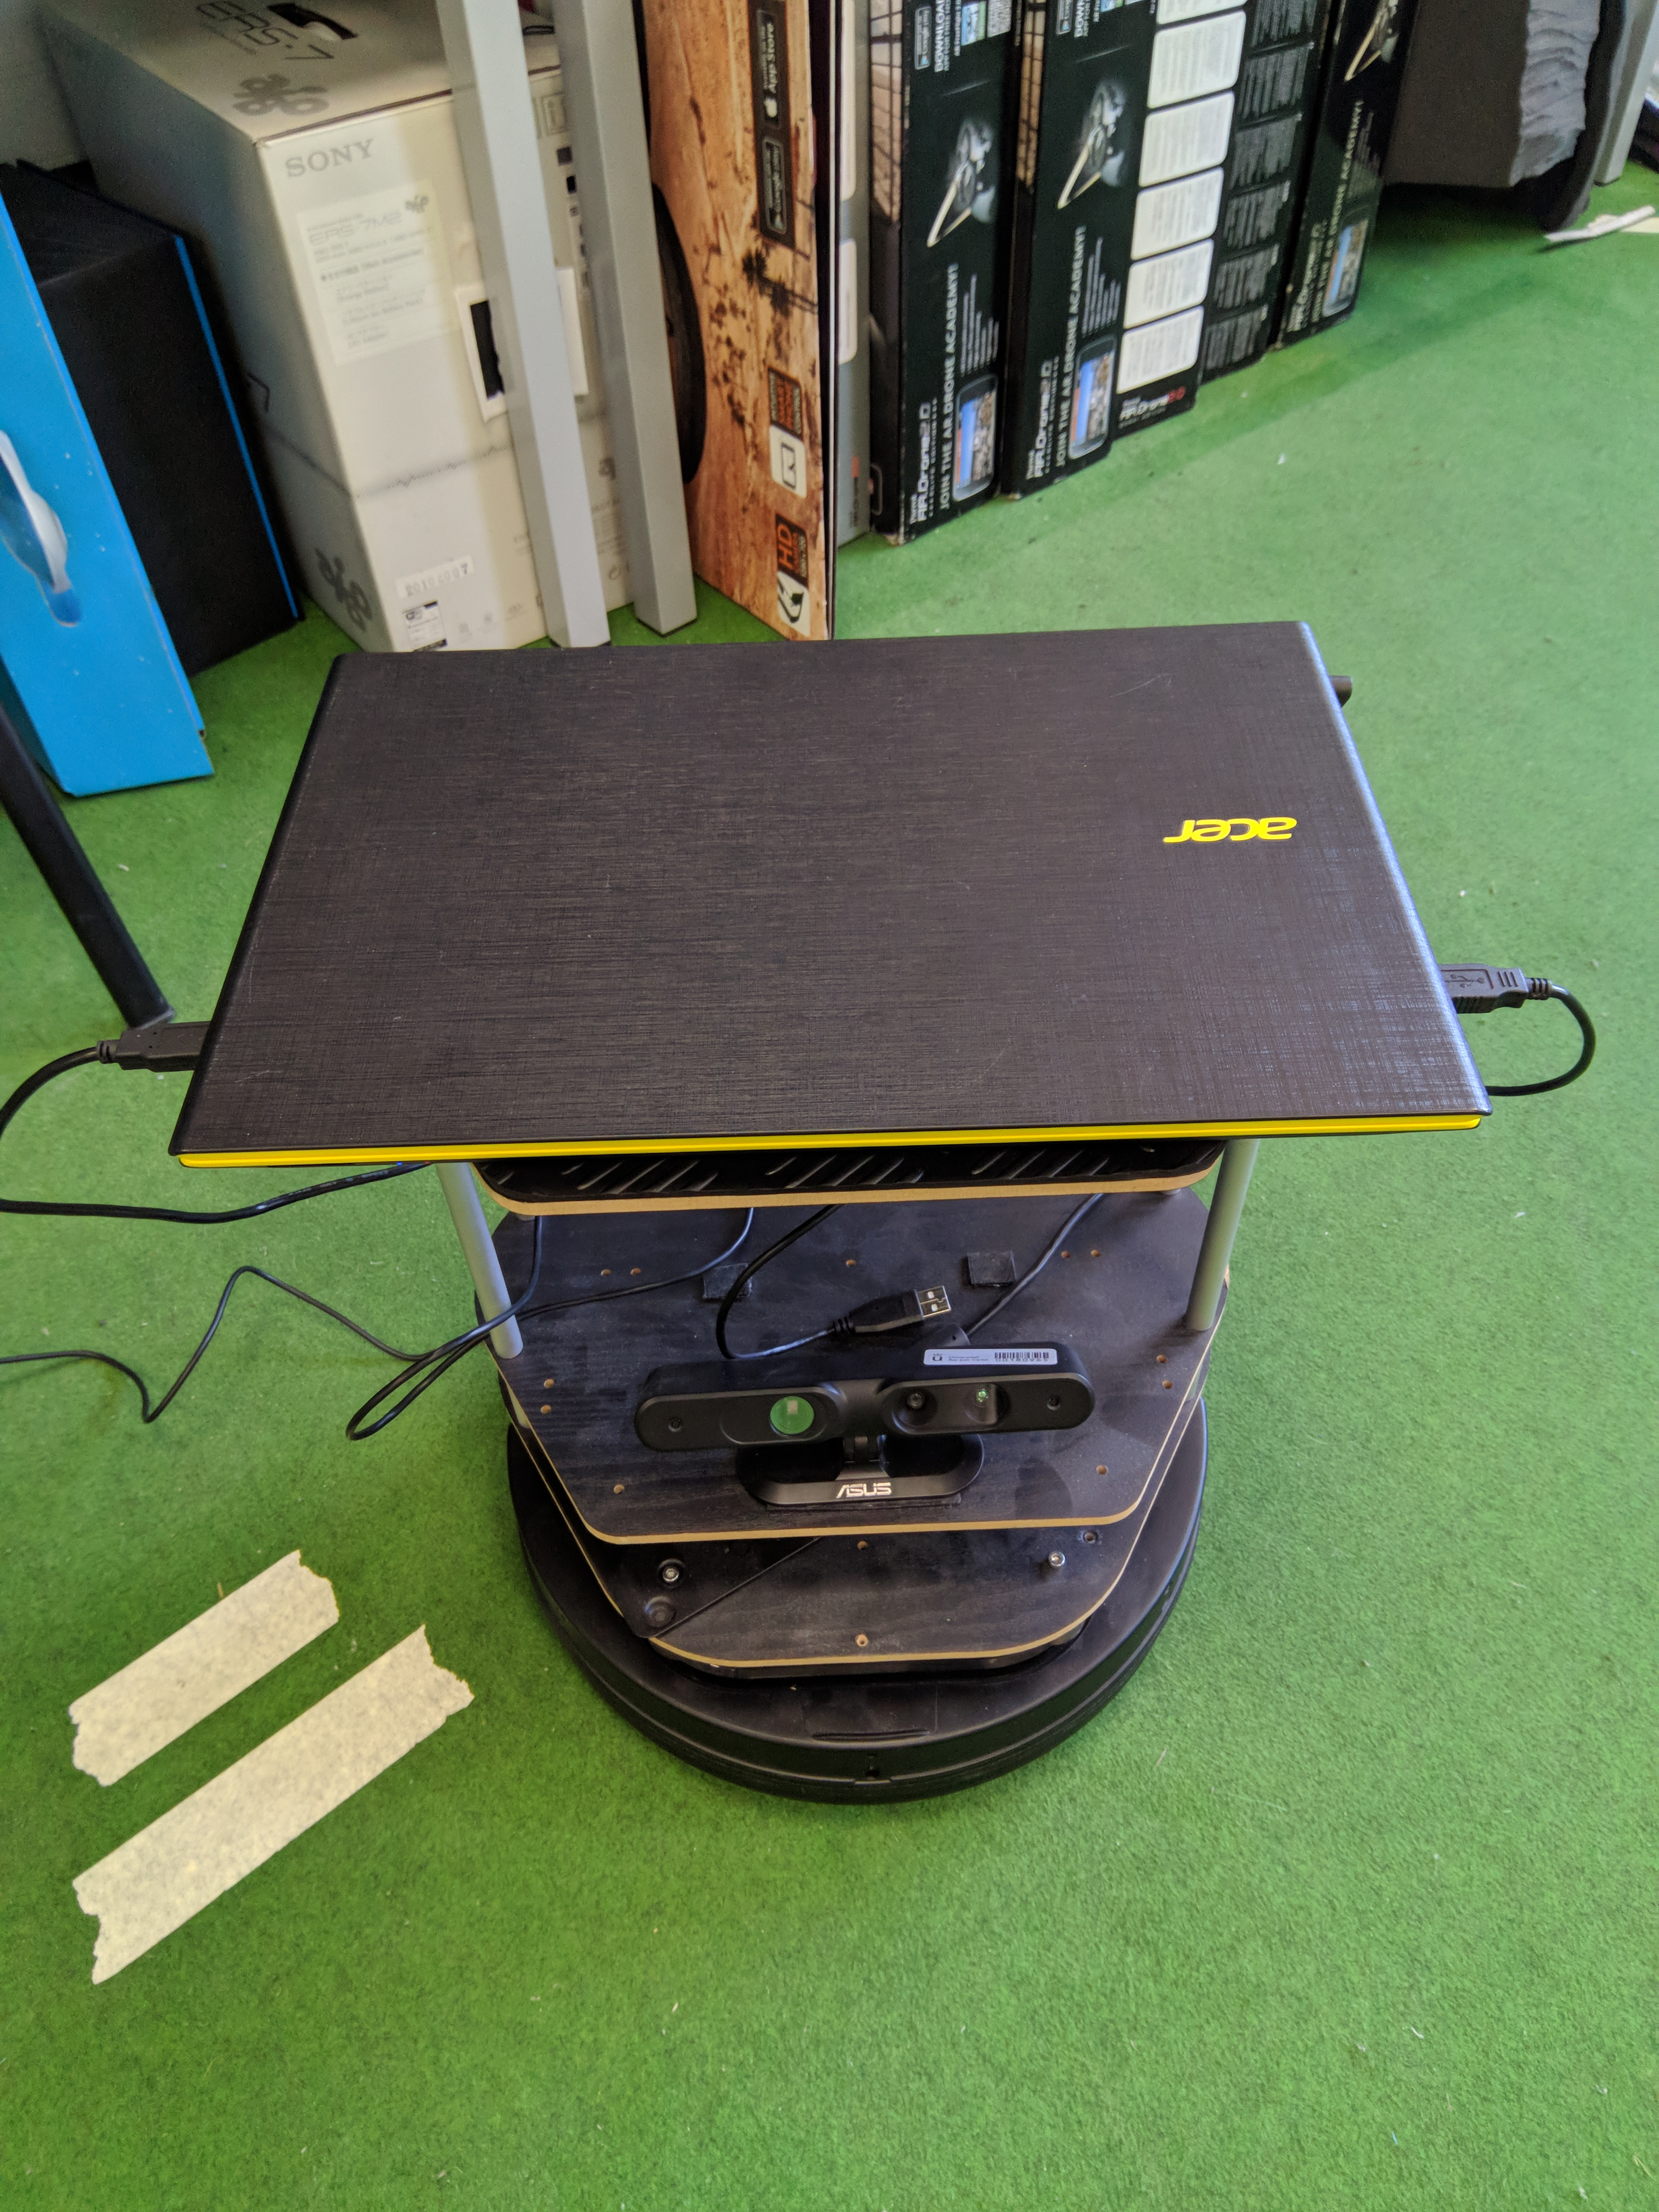
\includegraphics[width=1.9in]{tfg1}
		\caption{Frontal view.}
		\label{fig:3_turtlebot_front}
	\end{subfigure}
	\begin{subfigure}[h]{0.4\linewidth}
		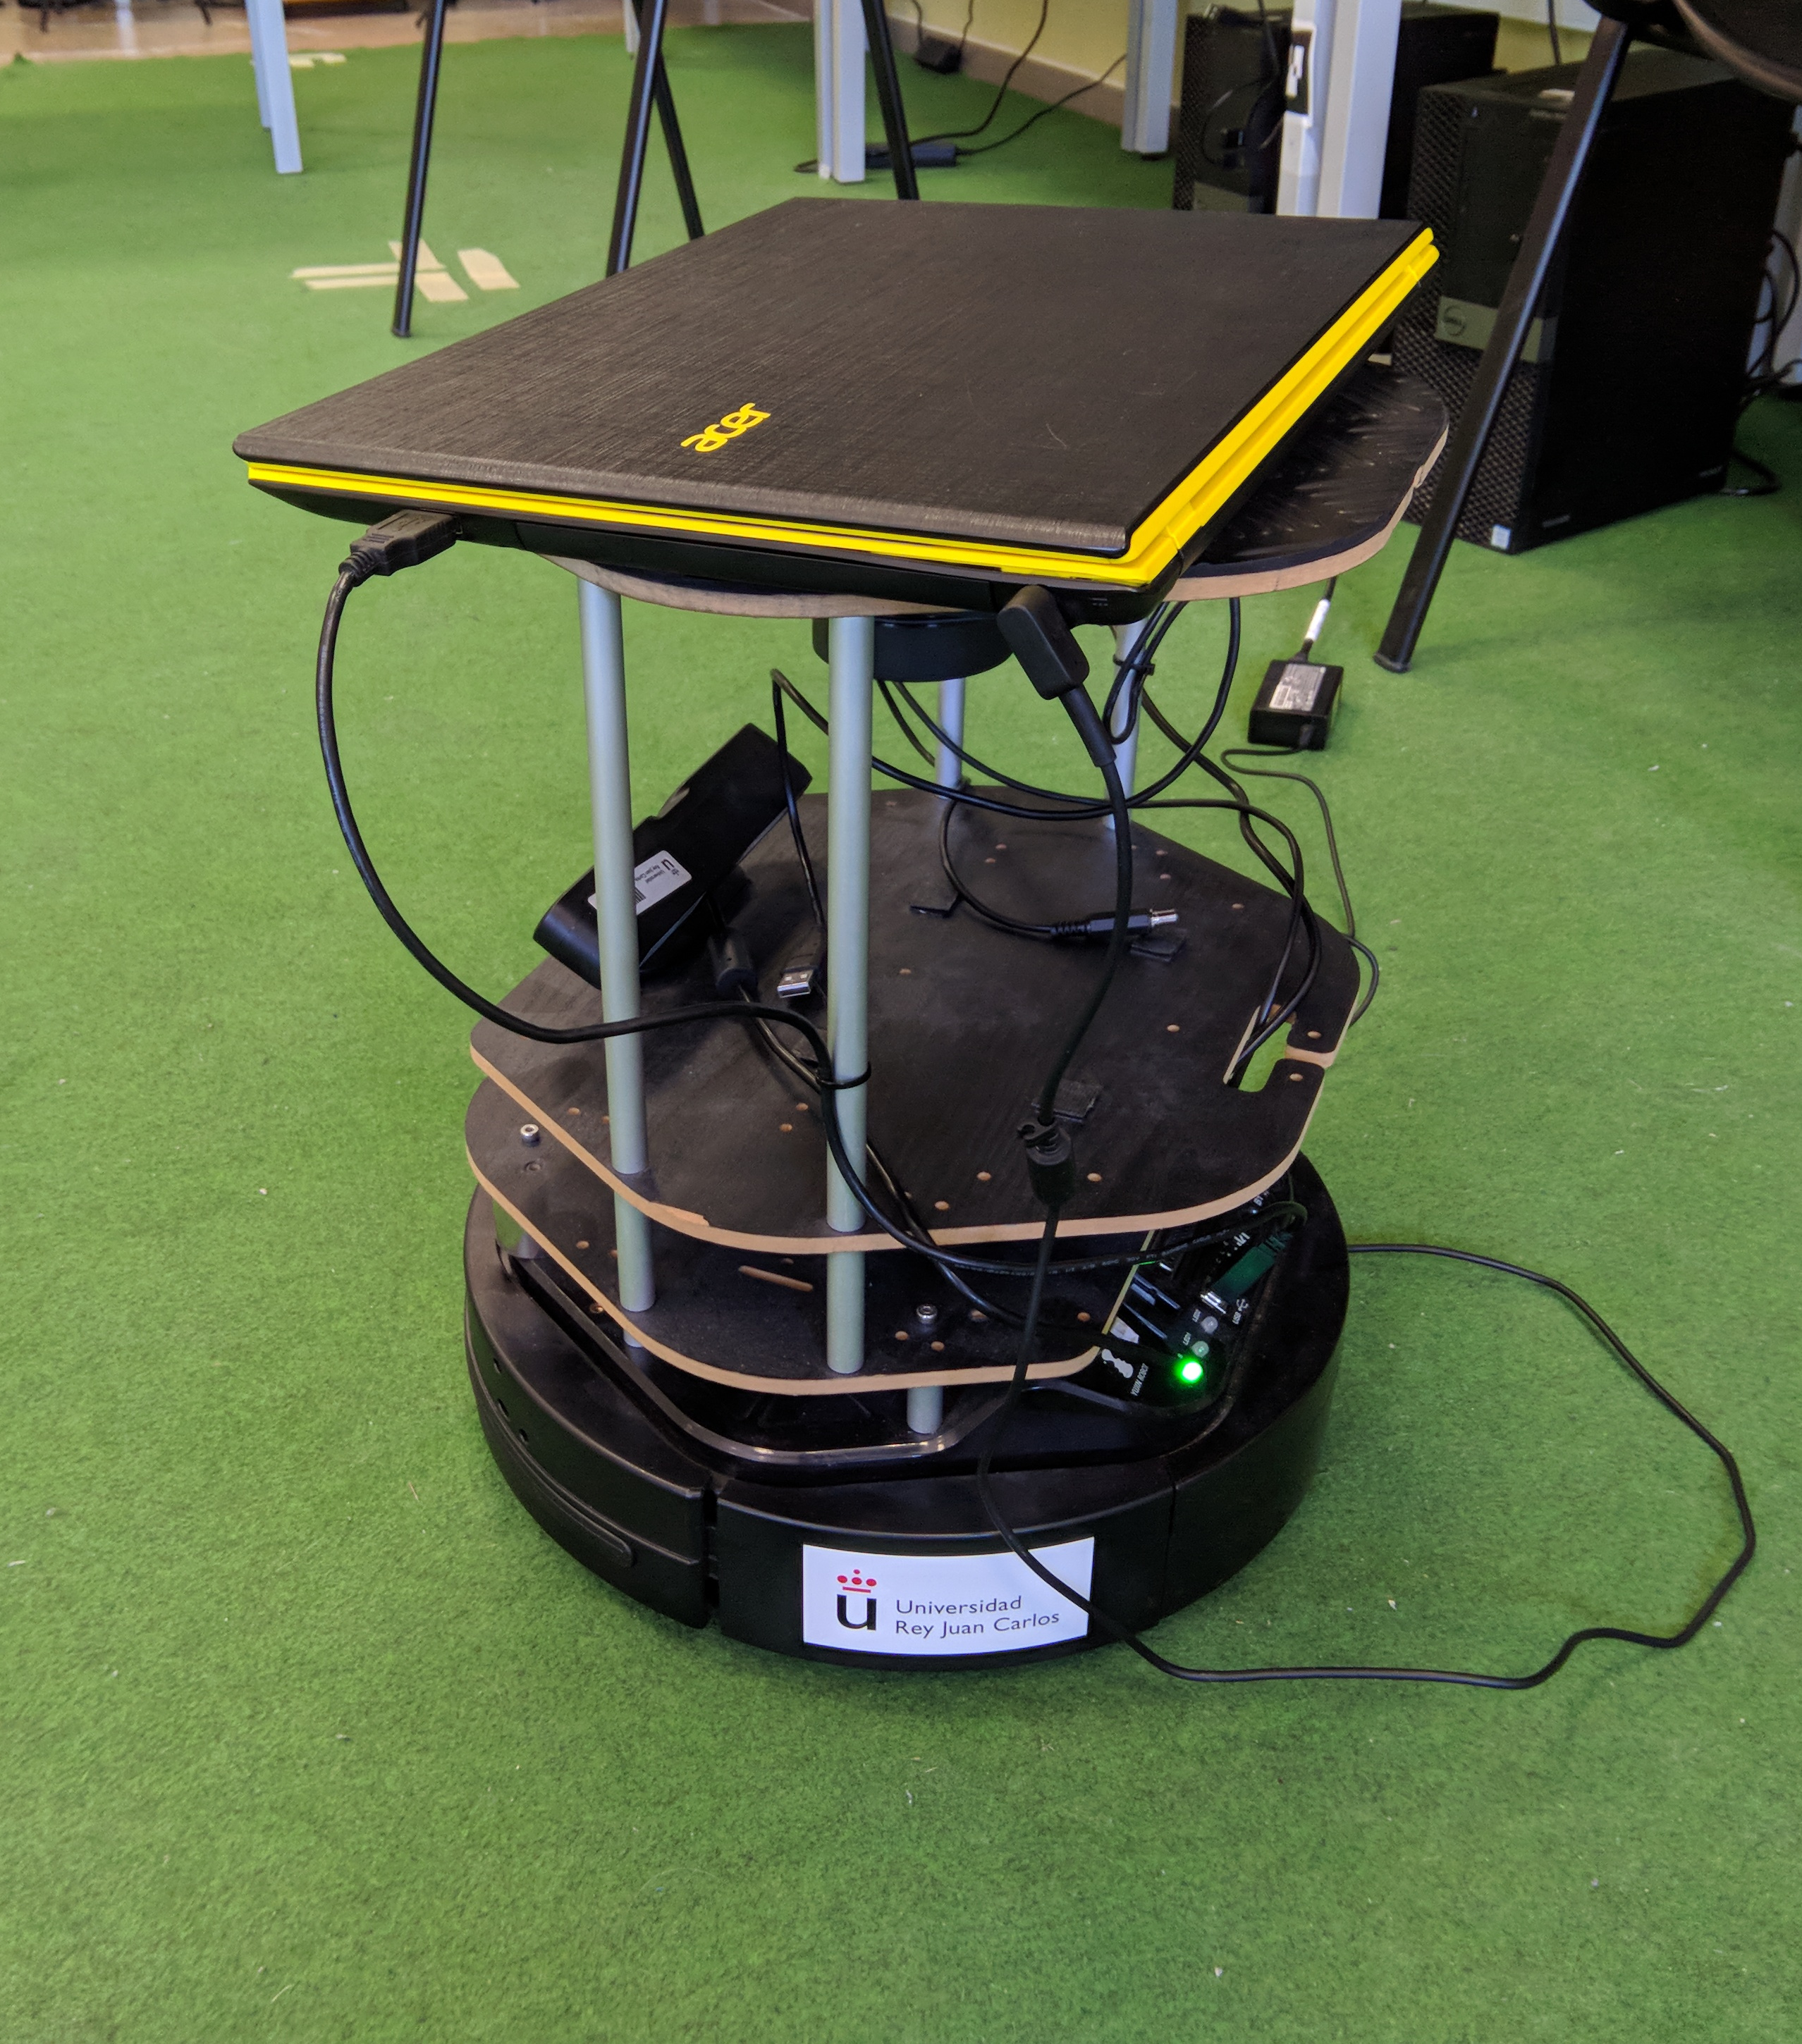
\includegraphics[width=2.2in]{tfg2}
		\caption{Side view.}
		\label{fig:3_turtlebot_side}
	\end{subfigure}
	\caption{Laptop+robot deployment on \cite{tfg}.}
	\label{fig:1_real_tfg}
\end{figure}

Nowadays, the mentioned increase in the interest into the real-time computer vision applications has fostered the development of specific low-power embedded devices to be integrated in mobile systems. The extending usage of devices such as Arduino or Raspberry Pi has led to embedded robotics systems, such as PiBot \cite{pibot} (\autoref{fig:1_pibot}). These robots are useful in the educational scope, as they are capable of running simple vision and navigation algorithms at a low cost.
\begin{figure}[h]
	\centering
	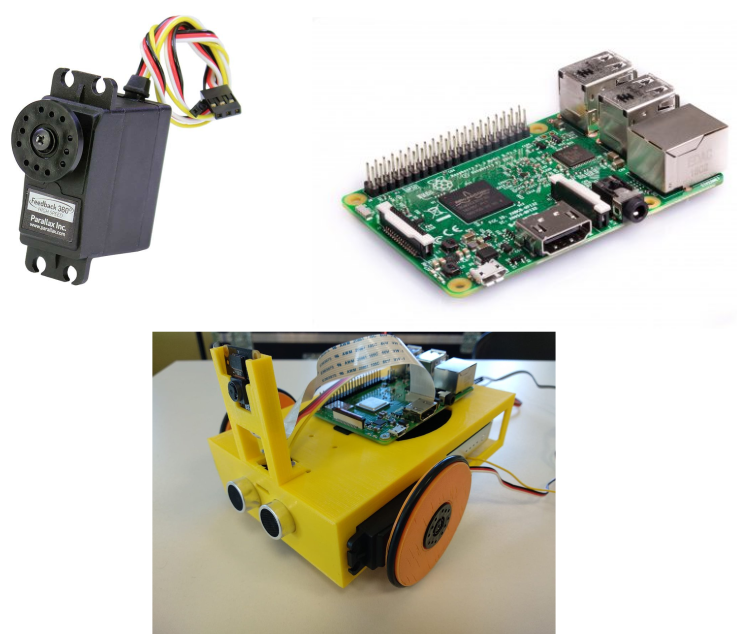
\includegraphics[width=0.5\linewidth]{pibot}
	\caption{PiBot, an open low-cost robotic platform for education (image from \cite{pibot}).}
	\label{fig:1_pibot}
\end{figure}
Unfortunately, the requirements on systems running more complex algorithms, such as neural networks, require of the next tier in power terms, keeping the portability nevertheless. The ideal device could be an ASIC, as the custom design would lead to a very tight optimization of the performance. However, we are aiming to run the algorithms on existing software frameworks, so we aim to general purpose computers instead. The most remarkable advance in this scope are the Jetson devices manufactured by NVIDIA. These development boards are SoM (\textit{System-on-Module}) computers running a tailored version of Linux. The fundamental feature of these systems is that they include a high-performance GPU featuring CUDA, a low-level parallel computation library, as well as several toolkits designed to optimize as much as possible the software implementations for the plethora of possibilities to be designed on this board. As it can be seen in \autoref{fig:1_tx2}, its size and power consumption make of this system a good choice to be included in an autonomous robotic system. 
\begin{figure}[h]
	\begin{subfigure}[h]{0.45\linewidth}
		\centering
		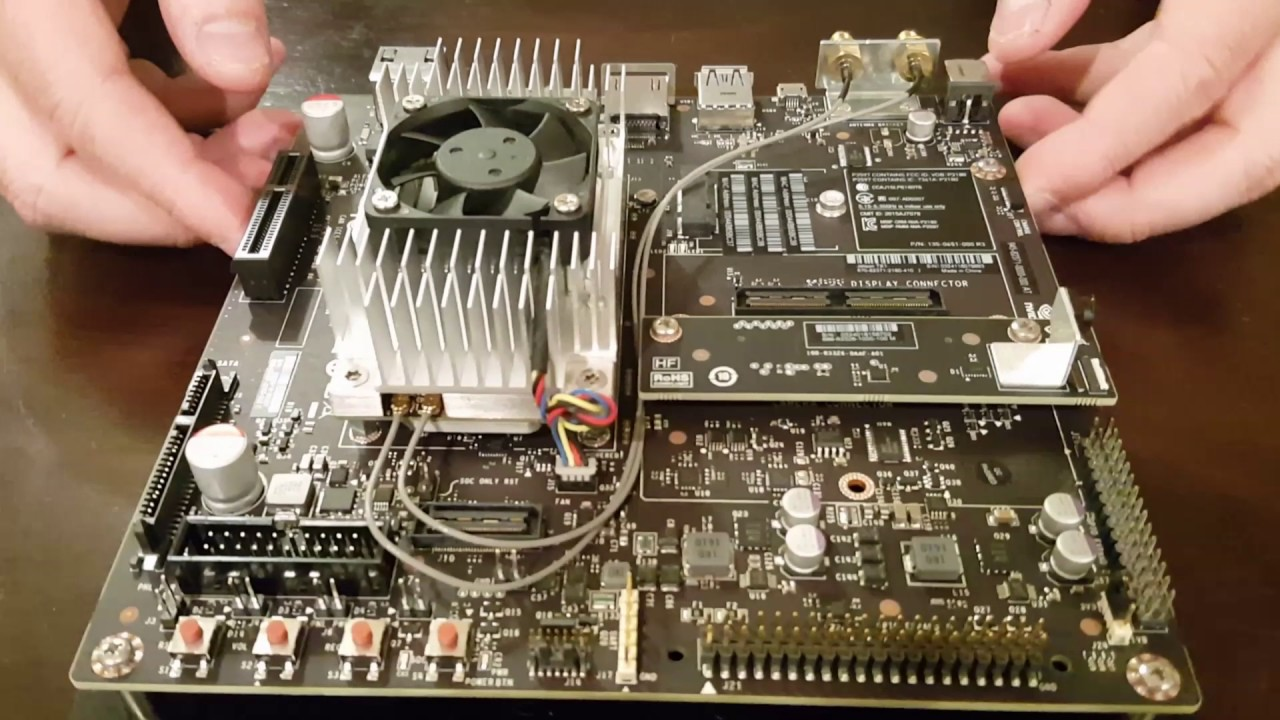
\includegraphics[width=\linewidth]{jetsontx2}

	\end{subfigure}
	\begin{subfigure}[h]{0.45\linewidth}
		\centering
		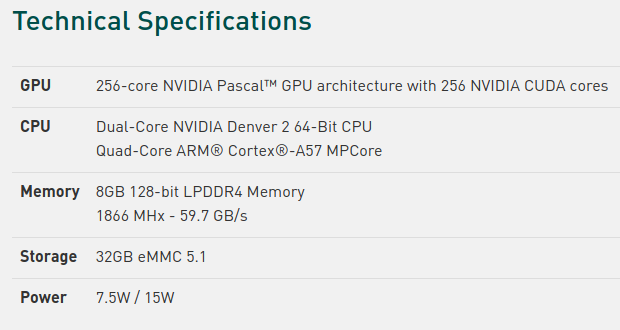
\includegraphics[width=\linewidth]{tx2_specs}
	\end{subfigure}
	\caption{NVIDIA Jetson TX2: an embedded high-performance device including a GPU.}
	\label{fig:1_tx2}
\end{figure}


\subsection{Person following}
Several approaches have been developing pursuing this challenge of \textit{following a person}. Once the perception algorithms are established, the final output of the pipeline has to be a movement command for the robot to move towards the desired point. Mobile  robots can be classified according to their locomotion capabilities. A good summary can be that a robot is \textit{holonomic} if the number of its controllable degrees of freedom is equal to its total degrees of freedom. If the controllable degrees of freedom are lower than the total degrees of freedom, the robot is \textit{non-holonomic}.\\

In the case of a holonomic robot, the navigation process is simplified, as the robot can instantaneously move to a desired target. However, a non-holonomic robot needs to perform maneuvers in order to move towards a point.\\

\section{Objectives}
\label{sec:1_objectives}
	This work has been carried out in order to fulfill certain requirements in a particular person following application:
	
	\begin{enumerate}
		\item Achieve a real-time following behavioral using embedded low-power hardware and a low-complexity educational robot.
		
		\item Build the inference pipeline using exclusively concurrent CNNs (\textit{convolutional neural networks}).
		
		\item Combine a neural system with probabilistic filtering to carry out a robust multimodal tracking of the persons in front of the robot. This will provide the system with extra endurance and robustness against detection losses/occlusions.
	\end{enumerate}
	
These objectives allow to summarize the starting point for the development of this project: the available materials are an educational robot equipped with a battery, an embedded \textit{SoM} and a RGB-D sensor.\\

The result will be an autonomous robot which will follow a specific person, whose face has to be known beforehand (using a \textit{reference face} image).

\chapter{State of the art}
\label{chap:2_sota}

This chapter delivers a review of the state of the art, to provide a general panorama of the problems and methods that this work addresses.\\

As it was previously introduced, this work is performed to explore the synergies on robotics and deep-learning-based visual perception. In this section, the current approaches and tools will be described in order to outline a general panorama where this work may be framed.\\

The problem to be addressed is to \textit{get a robot with a camera to follow a person}. This problem can be split into several steps, where different approaches have been previously proposed. These steps will be covered in the following sections.
	
\section{Visual person detection}
\label{sec:2_detection}
One of the most common approaches is known as the \textit{Viola-Jones} detector \cite{violajones}. This algorithm relies on a \textit{rigid body model}, which fits a specific shape. On a grayscale image, this shape can be typically distinguished by means of the pixel intensity levels. Although this method was originally designed to detect faces, the rigid body model allows to generalize its usage for detecting different objects, such as persons. With this purpose, several spatial filters called \textit{Haar features} (\autoref{fig:2_haarfeats}) are introduced: these are used across the image looking for the intensity pattern of each template, which should resemble a part of the rigid body. Since this detector provides a weak decision by itself, several filters (previously chosen in a training process) are combined on a \textit{boosted cascade} (\autoref{fig:2_violajones_boost}). A person is detected if the weighted combination of several filters are triggered inside a certain area, which is decided to potentially contain a person \cite{diapos_cv_clasif}.

\begin{figure}[h]
	\centering
	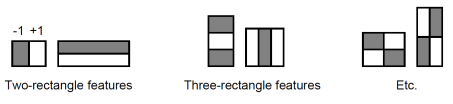
\includegraphics[width=0.7\linewidth]{haar_feats}
	\caption{Haar features: some examples \cite{diapos_cv_clasif}.}
	\label{fig:2_haarfeats}
\end{figure}

\begin{figure}[h]
	\centering
	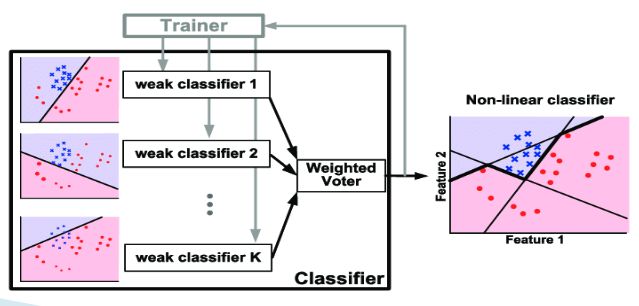
\includegraphics[width=0.7\linewidth]{boosted_cascade}
	\caption{Boosted weak classifiers \cite{diapos_cv_clasif}.}
	\label{fig:2_violajones_boost}
\end{figure}

The open-source standard image processing library, OpenCV, includes pre-trained models\footnote{\url{https://github.com/opencv/opencv/blob/master/data/haarcascades}}, which can be directly used with their Viola-Jones implementation. Scale invariance can be achieved evaluating the image at multiple scales on runtime.


Another common approach for person detection is based on HoG (\textit{Histograms of Gradients}) \cite{hog_detection}. This method computes local features by means of the intensity gradients across the image, and quantizes them according to their orientations (creating a histogram of oriented gradients for an image block), as it can be seen on \autoref{fig:2_hog}.\\



These gradients are collected in $64 \times 128$ windows, and treated as features. These features are evaluated by a linear SVM (\textit{Support Vector Machine}), which is trained to classify a window as \textit{person/non-person}. \autoref{fig:2_hog} shows the average gradient patch for a person (the direction of each gradient is not shown). A visual inspection immediately resembles the shape of a person standing up. Thus, this detector will yield the best performance when the person to be detected stands in that specific pose. This template allows as well to retain the gradients placed in the edges of the body (positive gradients), and discard those inside the body (negative gradients), weighting them according to their position inside the mentioned template.


\begin{figure}[h]
	\centering
	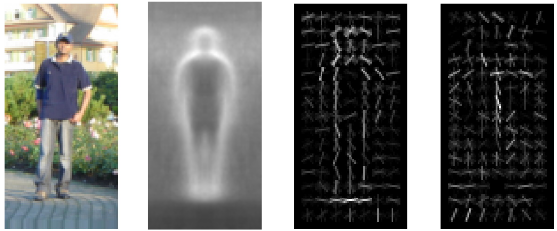
\includegraphics[width=0.7\linewidth]{hog}
	\caption{Example of the HoG computed for a person. From left to right: original image, average magnitude of the gradients on a person, directions weighted positive and negative gradients found in the input image. Image from \cite{hog_detection}.}
	\label{fig:2_hog}
\end{figure}




These methods, among several more, have been the state-of-the-art techniques: the cornerstone are the image gradients, which can be computed with a high efficiency, represented in a compact way by means of a histogram and provide decent performance. Their main drawback is the \textit{generalization} capability, as a successful detection is highly dependent on the person pose. However, in the latest advances, the detection techniques have moved towards the spreading paradigm: \textit{deep learning}, especially the most salient tools on image processing: CNNs (\textit{convolutional neural networks}).\\

CNNs are based on standard neural networks, which combine lots of neurons or \textit{perceptrons} organizing them into layers. These perceptrons (\autoref{fig:2_perceptron}) implement simple non-linear operations, that allow to extract (after a proper training process) abstract features, which gain in complexity when the number of internal layers increases. When a neural network is composed by many \textit{hidden} layers (in addition to the input/output ones), it is placed into the \textit{deep learning} paradigm (\autoref{fig:2_deep_learning}), as opposed to \textit{shallow learning}.

\begin{figure}[h]
	\centering
	\begin{subfigure}[t]{0.35\linewidth}
		\centering
		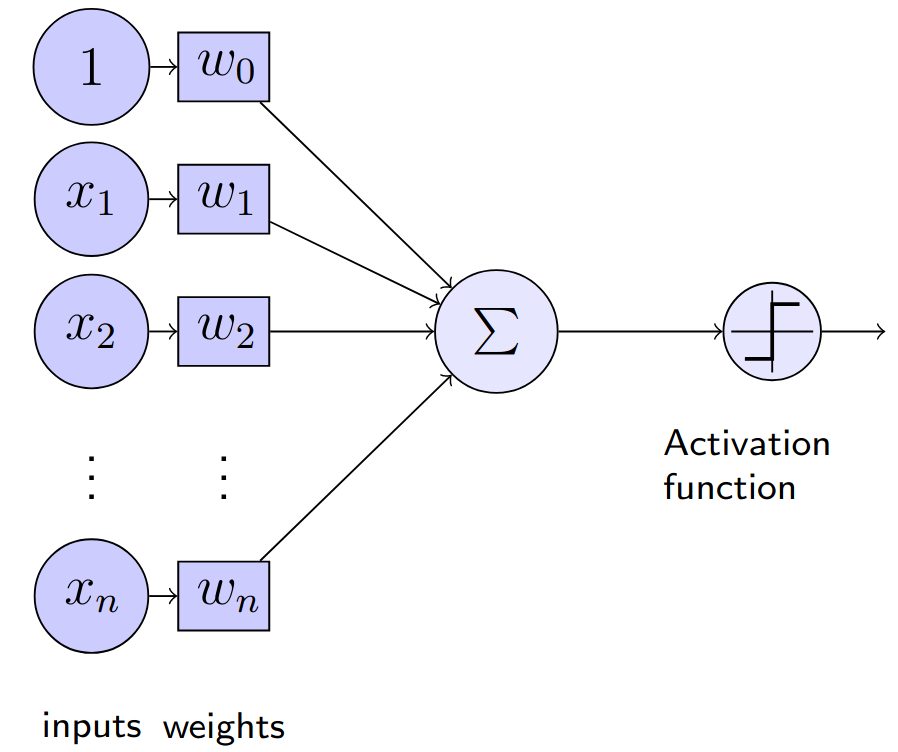
\includegraphics[width=0.95\linewidth]{perceptron}
		\caption{Basic unit of a neural network: the perceptron (source: \cite{tfg}).}
		\label{fig:2_perceptron}
	\end{subfigure}
	\begin{subfigure}[t]{0.5\linewidth}
		\centering
		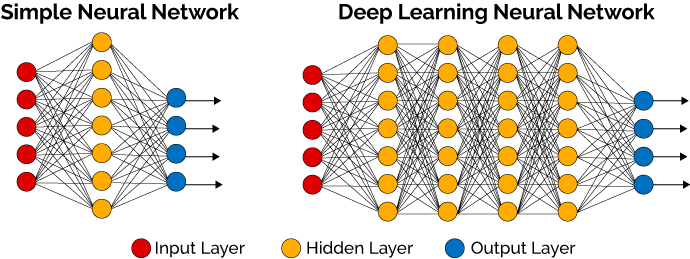
\includegraphics[width=0.99\linewidth]{deep_learning}
		\caption{Standard neural network vs. deep neural network (source: \cite{tfg}).}
		\label{fig:2_deep_learning}
	\end{subfigure}
	\caption{Basis of deep neural networks. (a), schematic of a perceptron. (b), increment on the number of hidden layers on deep learning approaches.}
	\label{fig:2_dnns}
\end{figure}


Based on this approach, and taking advantage of the \textit{spatial correlation} when the signal to process is an image, a neural network can be modified to implement a different operation on each perceptron: a \textit{convolution} (\autoref{fig:2_convolution}).

\begin{figure}[h]
	\centering
	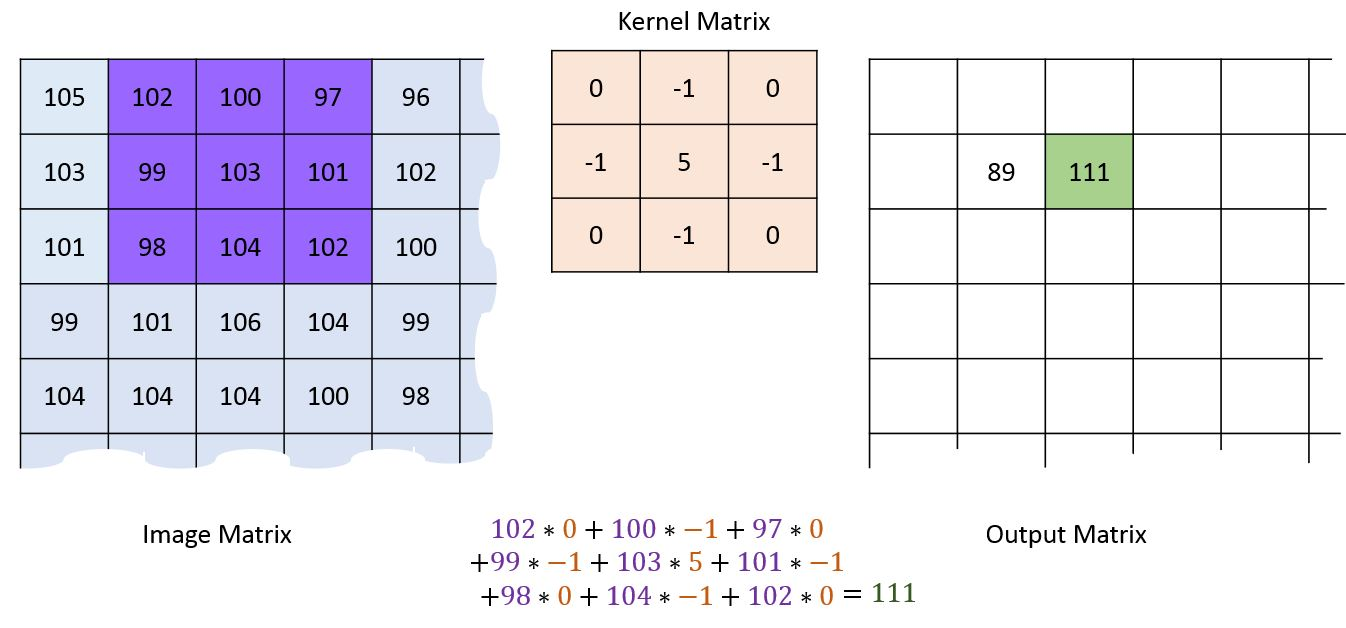
\includegraphics[width=0.7\linewidth]{convolution}
	\caption{Convolution applied to an image, applying the mask (red) on a region  (purple) of the input image, storing the result on the mapping of the central pixel of the region (green). The computation is the sum weighted by the mask values (bottom) (source: \cite{tfg}).}
	\label{fig:2_convolution}
\end{figure}

As it can be seen on \autoref{fig:2_cnn}, convolutional units may be arranged conforming a set of layers to build \textit{feature extraction} stages (shown in red in the figure). Several layers can be concatenated, gaining in depth and obtaining more complex feature maps. These layers are finally followed by a detection/classification ensemble of \textit{dense} layers (shown in blue in the figure): a set of layers with standard perceptrons fully-connected among them, yielding a final output, dependent on the classification structure of the network.

\begin{figure}[h]
	\centering
	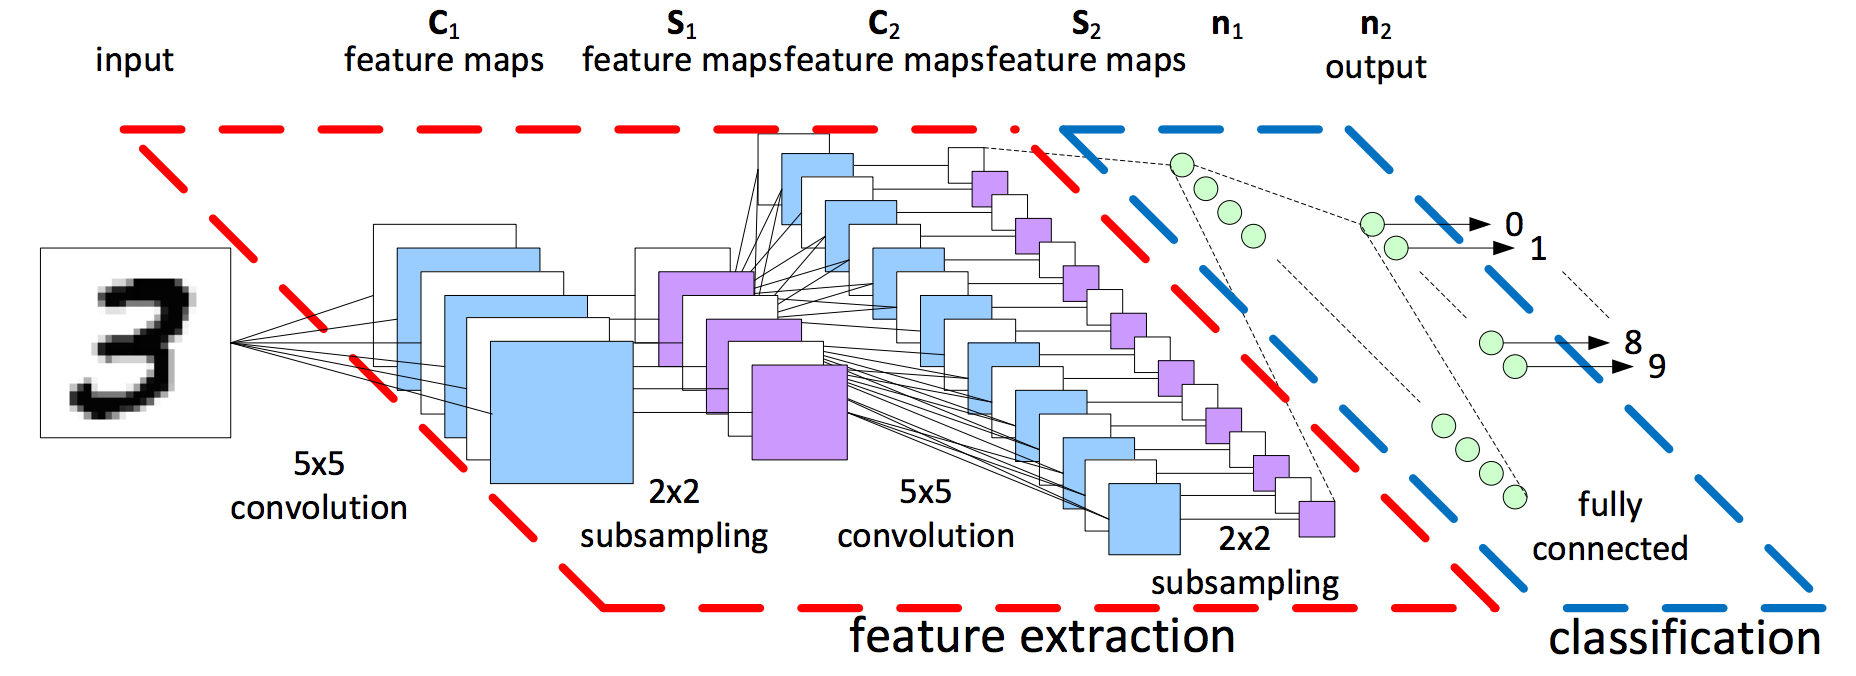
\includegraphics[width=0.9\linewidth]{cnn_architecture}
	\caption{Schematic of a digit classification CNN (source: \cite{tfg}).}
	\label{fig:2_cnn}
\end{figure}


In the case of object detection networks (the ones involved in this work), the output varies depending on the implementation, but it is generally composed of a set of \textit{(location, probability)} tuples, one for each class the network is capable of detecting. \autoref{fig:2_activation_maps} shows the activation maps of an object detection network, where the map presents higher values in the regions with high probability of containing the object of the class it is designed for. On a convolutional layer, each neuron computes several activation maps across the dimensions of the input data.

\begin{figure}[h]
	\centering
	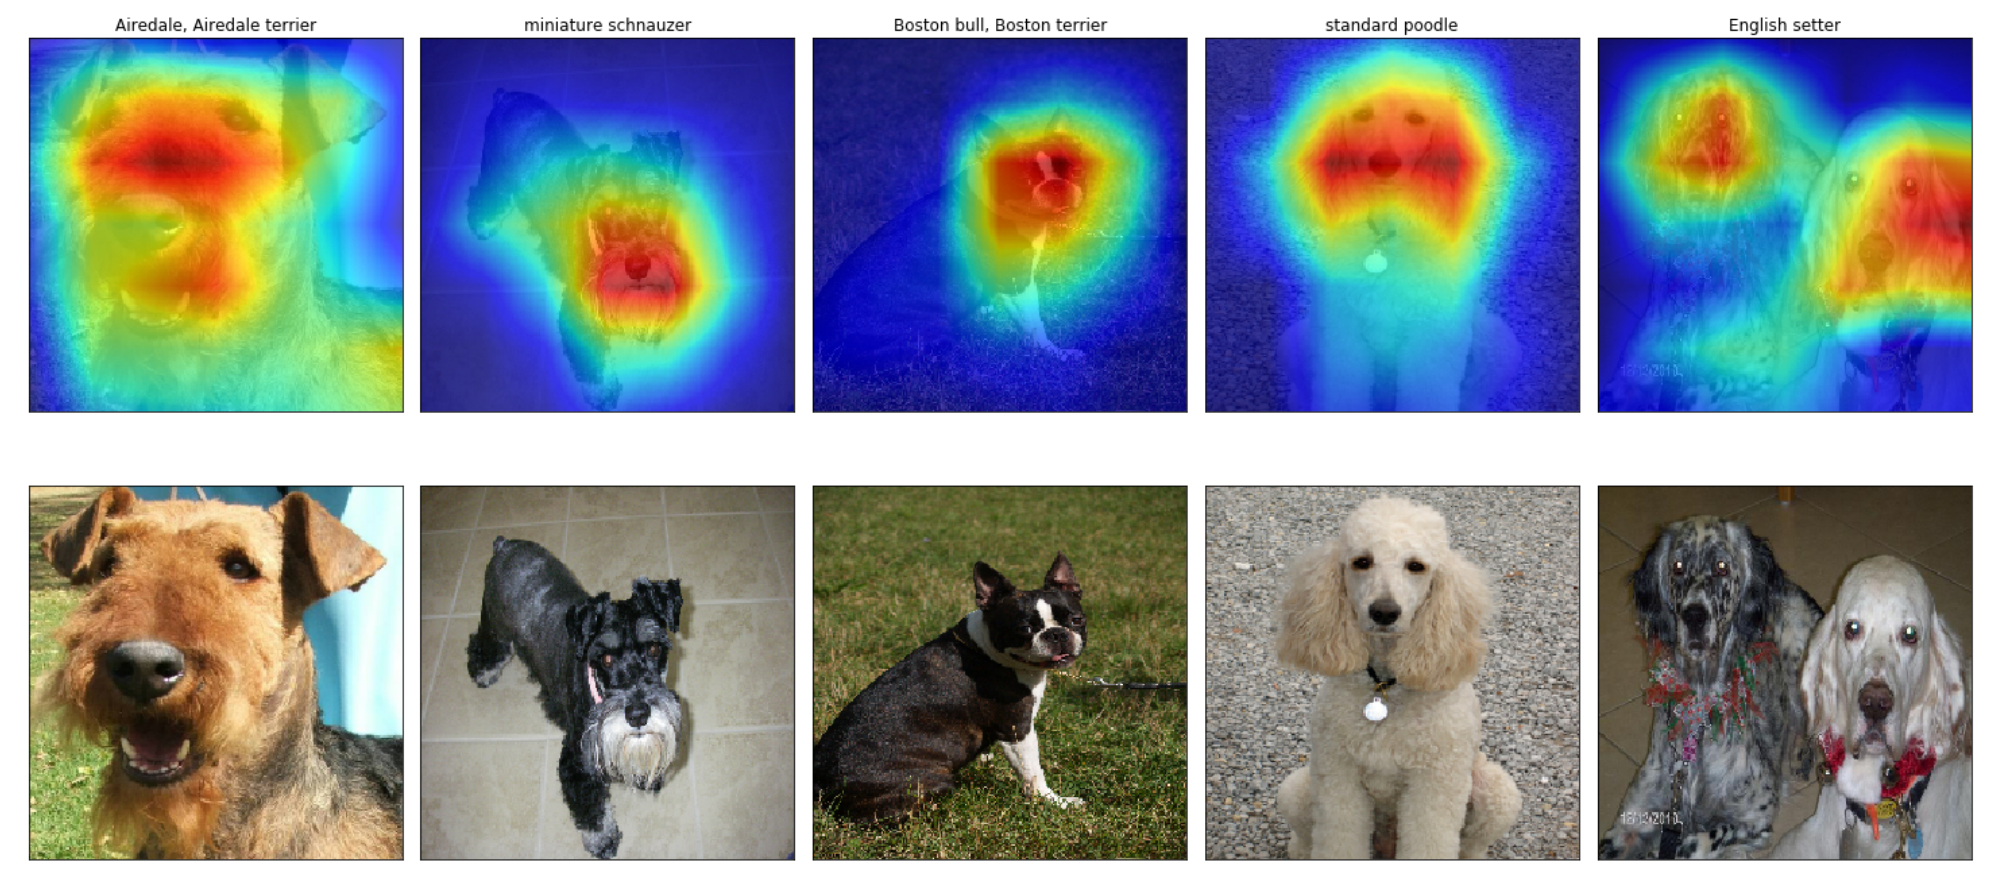
\includegraphics[width=0.9\linewidth]{activation_maps}
	\caption{Activation maps of a detection CNN searching for dogs on different images (source: \cite{tfg}).}
	\label{fig:2_activation_maps}
\end{figure}


One possible application of this concept is focused on what is called \textit{Region-based Convolutional Neural Networks} (R-CNNs) \cite{rcnn}, which require a previous step on the image called \textit{region proposal}. This step is devoted to find potential regions on the image to contain an object. This way, the challenge is to label these regions according to the objects contained inside, reducing the problem to a classification task. However, the process to find these regions and iterate over them makes the process too slow for real-time requirements, which are explicitly considered in our requirements. A notable effort has been made in later works \cite{fastrcnn} \cite{spp} to reduce this computation time.\\



\subsection{Single-Shot Multibox Detector (SSD)}
\label{sec:2_ssd}
Another outstanding object detection architecture is SSD (\textit{Single-Shot Multibox Detector}) \cite{ssd}. The main benefit from this architecture is the fact that it embeds all the required computations in a single neural network, reducing the complexity compared to other approaches requiring external region proposals, as it was explained above. This greatly reduces the computational time when the network has to process an image. The architecture can be seen at \autoref{fig:2_arch_ssd_yolo}, and can be split into several stages \cite{tfg}, namely:

\begin{description}
	
	\item[Reshape:] the first task to be addressed by the network is to reshape the input image(s) to a fixed size on which the rest of the layers work. In the case of an SSD detector, this shape is $n \times 300 \times 300 \times 3$ (being $n$ the size of the input batch, as $n$ images can be evaluated simultaneously on the neural network). Other image sizes might be used, however this one offers a good trade-off between performance and computational load.
	
	\item [Base network:] this first group of layers are reused from a typical image classification model, such as VGG-16 \cite{vgg16}. The first layers of this architecture are utilized in this design, truncated before the first classification layer. This way, the network can leverage the \textit{feature maps} from the classification network, in order to find objects inside the input image. Following the first part of the network, several convolutional layers are appended, decreasing in size. This has the objective of predict detections at multiple scales. One thing to mention at this point is that the base network can be a different one rather than VGG-16, such as a MobileNet \cite{mobilenet}, which is highly optimized for running on low-end devices. This is interesting as our embedded system will be limited in computing power. It will be revisited in future sections.
	
	\item[Box predictors:] for each layer in the base network, an image  convolution is performed, generating a small set (typically 3 or 4) of fixed-size \textit{anchors}, with varying aspect ratios for each cell on a grid over the activation map (\autoref{fig:2_ssd_generated_boxes}). As these maps have different sizes, the system is able to detect  objects in different scales. The anchors are then convolved with small filters (one per depth channel), which output confidence scores for each known class, and offsets for the generated bounding box. These scores are passed through a \textit{softmax} operation, that compresses them into a probability vector. Thus, for each detected object (on that scale), the network computes the score on every class and its estimated position inside the feature map (hence, in the image as well).
	
	\item [Postprocessor:] as several detections might be triggered in the same area for different classes and scales, a \textit{Non-Maximum-Supression} \cite{nms} operation is performed at the output of the network to retain the best boxes, under a combined criteria of detection score and IoU score (\textit{Intersection over Union}), which measures the overlapping quality between two bounding boxes, as it can be seen in \autoref{fig:2_iou}.
\end{description}


\begin{figure}[h]
	\centering
	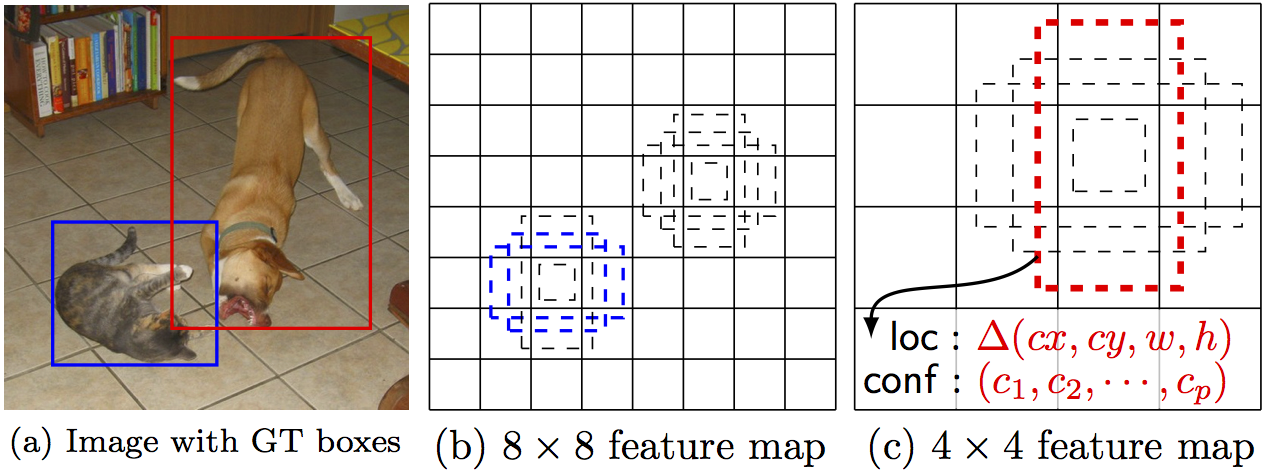
\includegraphics[width=0.7\linewidth]{ssd_generated_boxes}
	\caption{A set of boxes are generated centered on each point of every feature map \cite{ssd}.}
	\label{fig:2_ssd_generated_boxes}
\end{figure}

\begin{figure}[h]
	\centering
	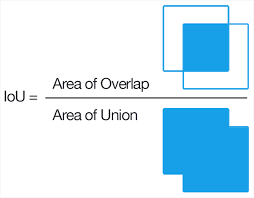
\includegraphics[width=0.4\linewidth]{iou}
	\caption{Graphical representation of the IoU score between two bounding boxes.}
	\label{fig:2_iou}
\end{figure}

\subsection{YOLO (You Only Look Once)}
\label{sec:2_yolo}
Another interesting approach is the YOLO (\textit{You Only Look Once}) system \cite{yolov1}. Its main advantage is its inference speed, due to the fact that it performs a single analysis on the entire image, dividing it into a grid of cells. Each cell predicts up to 5 boxes, containing an \textit{objectness score} (the predicted IoU of the proposal with an object, regardless its class), the coordinates of the bounding box, and a probability for the object belonging to each class. This design run faster than other methods \cite{yolov1}, however it presents a poor performance when detecting small objects.\\

This design was revisited in YOLO9000 \cite{yolov2}, introducing several improvements such as batch normalization at the input of the convolutional layers, or the concept of \textit{anchor boxes}: the box proposals follow a fixed set of aspect ratios, chosen previously using clustering on a training set. As it can be seen on \autoref{fig:2_yolov2_anchor_clustering}, limiting the proposal shapes to 5 fixed sizes improves the performance while maintaining a high IoU metric. A visual inspection shows that the selected anchors seem like a reasonable shape for the majority of the objects the network aims to detect. Additionally, the number of deep layers was increased from 26 layers to 30, and a semantic modeling is performed on the labels across different datasets, allowing the network to be trained in different datasets under a common semantic structure called \textit{WordTree} (\autoref{fig:2_yolov2_wordtree}).

\begin{figure}[h]
	\centering
	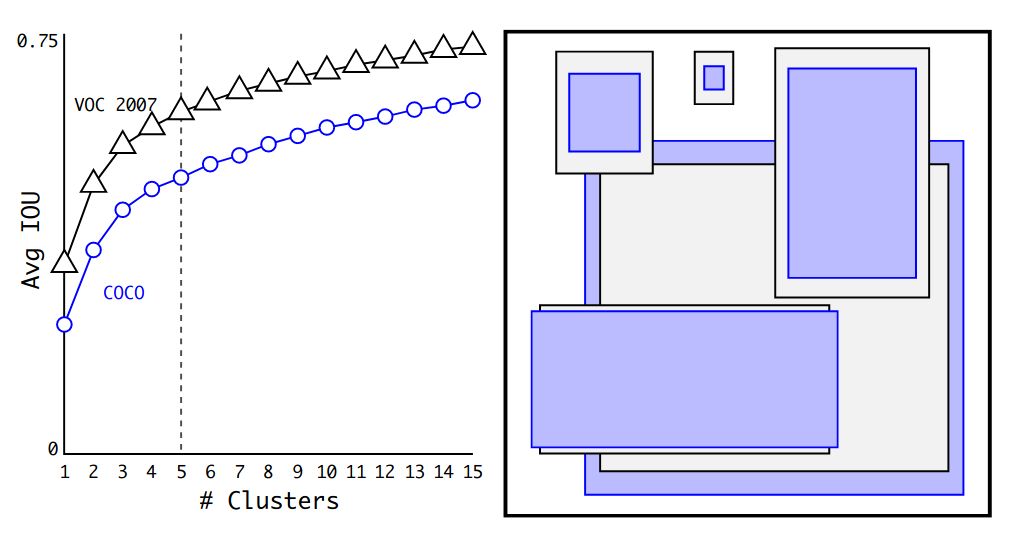
\includegraphics[width=0.6\linewidth]{yolov2_anchor_clustering}
	\caption{Result of the anchor k-means clustering on VOC and COCO for YOLO9000. Using $k=5$ anchor sizes on the right yields a good tradeoff between simplicity and improvement on the obtained IoU with respect to using $k-1$ clusters (source: \cite{yolov2}).}
	\label{fig:2_yolov2_anchor_clustering}
\end{figure}
%\vspace{20cm}


\begin{figure}[h]
	\centering
	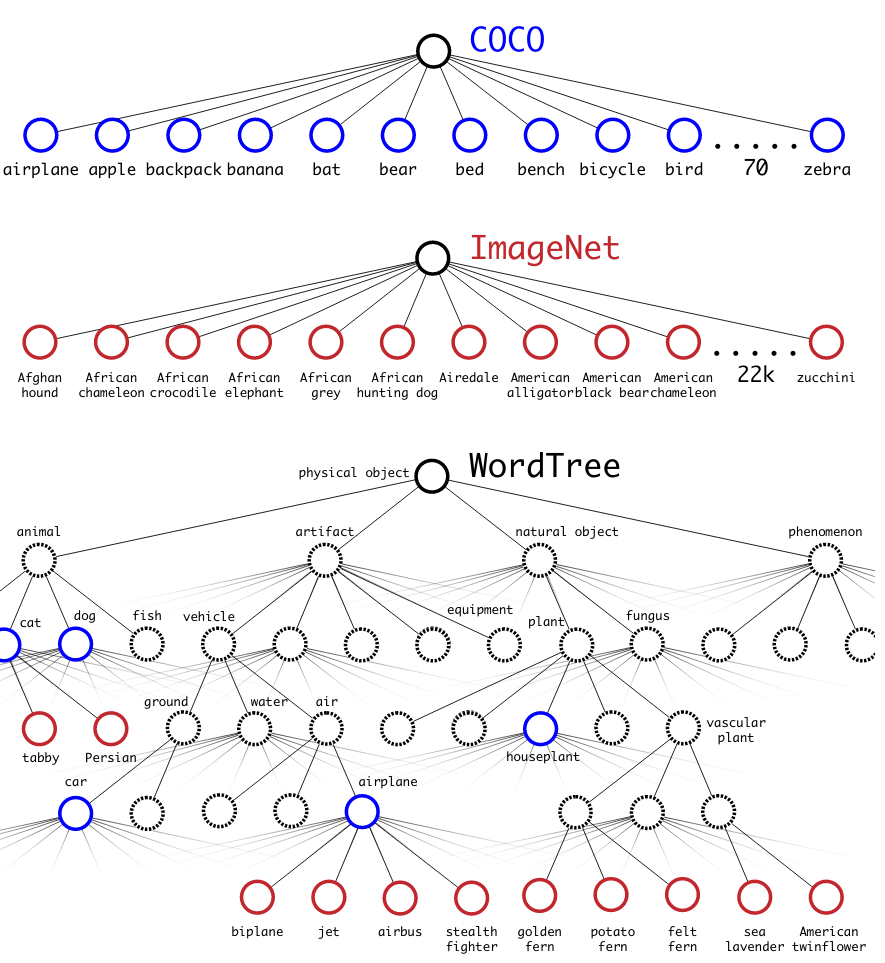
\includegraphics[width=0.6\linewidth]{yolov2_wordtree}
	\caption{Comparison between simple labeling structures (top) and a WordTree semantic grouping under categories (bottom). This allows to follow a dataset-agnostic training process as the labels can be combined using WordTree. Image from \cite{yolov2}.}
	\label{fig:2_yolov2_wordtree}
\end{figure}




The latest improvement of YOLO, YOLOv3 \cite{yolov3}, relies on residual networks \cite{resnets}, which tackle the problem of \textit{vanishing gradients} when the networks become deeper. The stacking of several layers results on gradients diminishing its value up to a point the arithmetical precision of the machine is not able to handle. The gradients are canceled, hindering the training process, as the first layers parameters take a substantially higher time to converge. The residual networks added in this revision of the design add shortcut connections across the layers, focusing the backpropagation gradients on the differences between the input and the output of the layer. As this reference states \cite{yolov3}, the combination of these residual layers and convolutional ones allows to train much deeper architectures (53 convolutional layers), capable of yielding a higher generalization. As in the SSD detectors, the YOLO architecture performs multi-scale detections, using 3 scales for splitting the feature maps into cell grids. A similar k-means clustering than in \autoref{fig:2_yolov2_anchor_clustering} is performed on the COCO dataset, selecting 9 anchor sizes instead of 5, and grouping them in 3 scales. Now, on each of the cells, 9 anchor bounding boxes are fit (3 anchor shapes $\times$ 3 scales). This aims to improve the poor performance of the previous version when dealing with small objects, as well as to produce better generalization: in the R-CNN \cite{rcnn} and the SSD \cite{ssd} the anchor shapes are hand-picked. These changes, with a tuning on the error function, conform the YOLOv3 improvements over the previous versions.\\

\vspace{5cm}

For each \textit{(anchor, cell, scale)} combination, YOLOv3 predicts:

\begin{itemize}
	\item The coordinates of the object within the anchor. Details can be visualized on \autoref{fig:2_yolo_output}.
	
	\item \textit{objectness} score, which is computed by means of a logistic regression in order to maximizing the probability of overlap with a ground truth bounding box with respect to that of any other prior anchor.
	
	\item 80 scores, as the original implementation is trained in the COCO dataset, which contains 80 classes. These classes might be overlapping (e.g. ``woman'' and ``person''). Thus, these scores are computed by independent logistic classifiers and are not passed through a \textit{softmax} operation.
\end{itemize}


\begin{figure}[h]
	\centering
	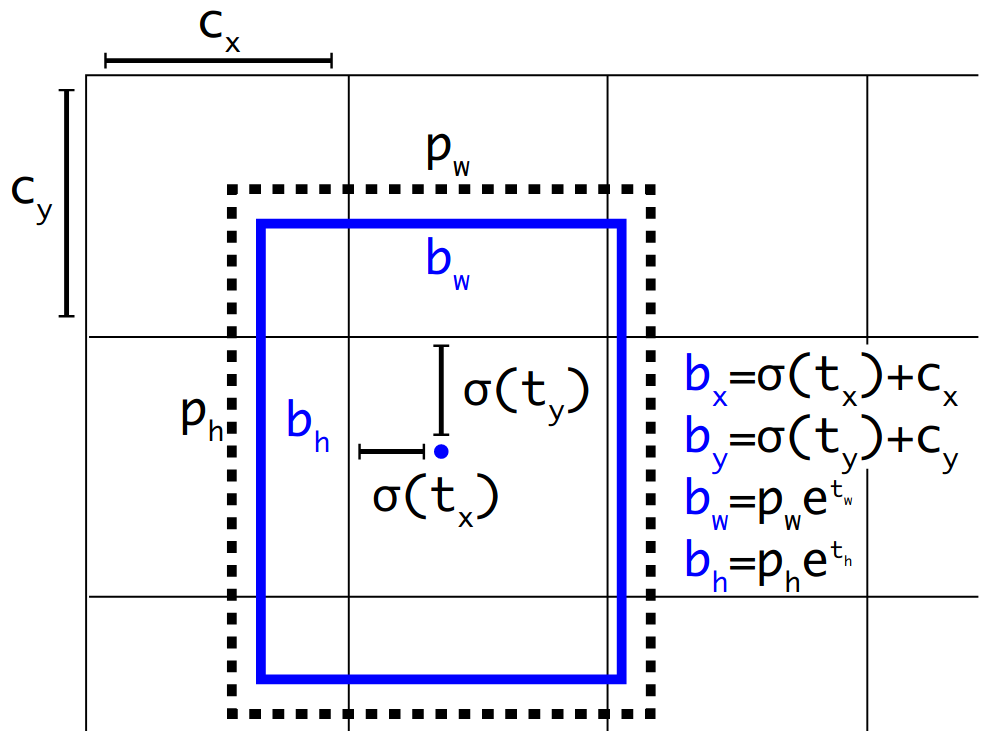
\includegraphics[width=0.5\linewidth]{yolo_outputs}
	\caption{Output on YOLO for each anchor and cell. The dashed line represents the prior anchor, while the blue line represents the detection which corrects that anchor.}
	\label{fig:2_yolo_output}
\end{figure}


The architecture of a YOLO-based detection network can be compared to that of a SSD-based one in \autoref{fig:2_arch_ssd_yolo}. This allows to see the fundamental difference in the feature extraction stage of each approach.

\begin{figure}[h]
	\centering
	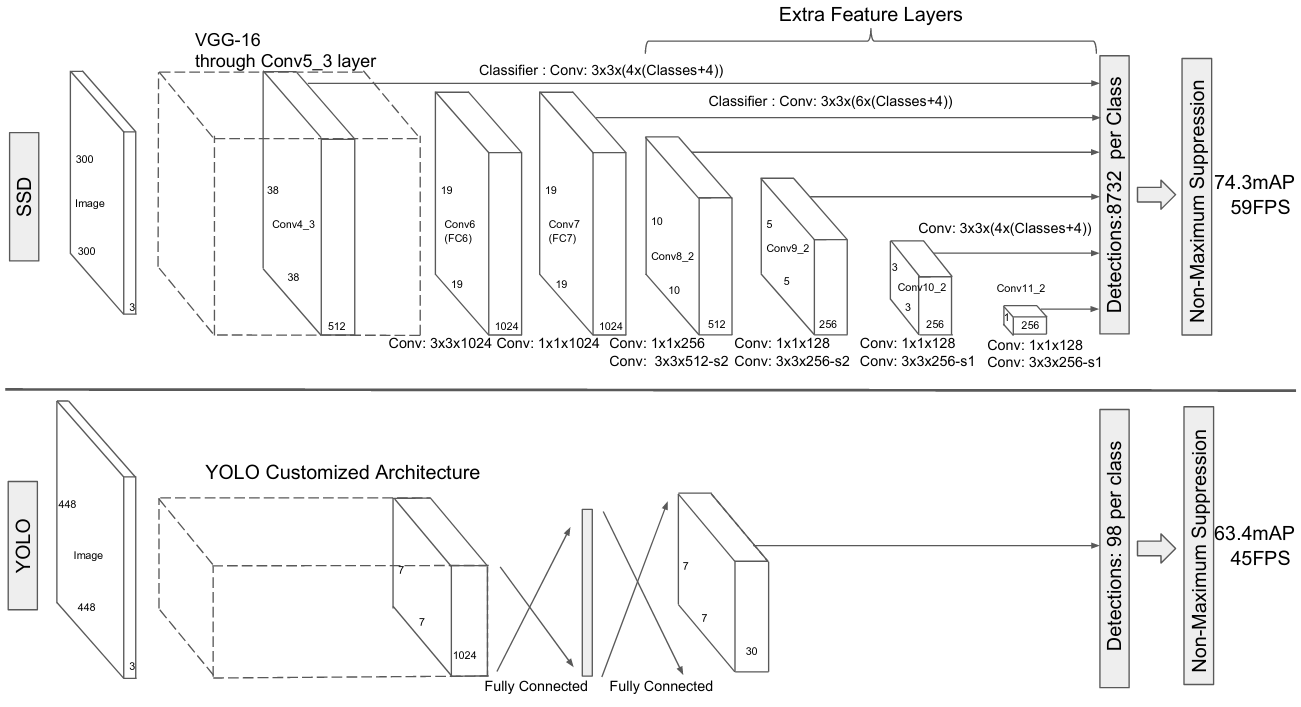
\includegraphics[width=0.8\linewidth]{arch_ssd_yolo}
	\caption{General architecture of a SSD network (top) and a YOLO one (bottom). Image from \cite{ssd}.}
	\label{fig:2_arch_ssd_yolo}
\end{figure}

\newpage
\section{Person identification}
\label{sec:2_ident}
On a controlled environment, where the only present person is the one to be followed, a person detection system could be enough for following purposes. However, in a real scenario, there might be several people inside the field of vision of the robot. This problem can be approached by means of a distinguishing feature of the person of interest, provided beforehand. One example is \cite{color_id}, which computes the color distribution of the person of interest, and later compares this distribution with the ones belonging to the different persons using the Bhattacharyya coefficient \cite{bhattacharyya} (a measurement of similarity between two probability distributions). This metric can be applied for computing the similarity between the color histograms of the reference person and the detected one. However, this system can be deceived replicating the color distribution of the person of interest: wearing similar clothes helps to reduce the distance between the histogram, leaving a chance to confound another person with the one to follow.\\

A more robust approach is to use the \textit{face} of the person as the discriminant feature, as its uniqueness makes it a good reference to identify the detected person. As it is summarized in \cite{dlib_review}, several applications extract facial \textit{landmarks} from the morphology of a given face (\autoref{fig:2_dlib_landmarks}), and use them to recognize the face, comparing it with a set of known faces and estimating the identity based on the distance to each known face. Some open-source libraries such as \texttt{dlib} and \texttt{OpenCV} provide algorithms to perform these processes.\\

\begin{figure}[h]
	\centering
	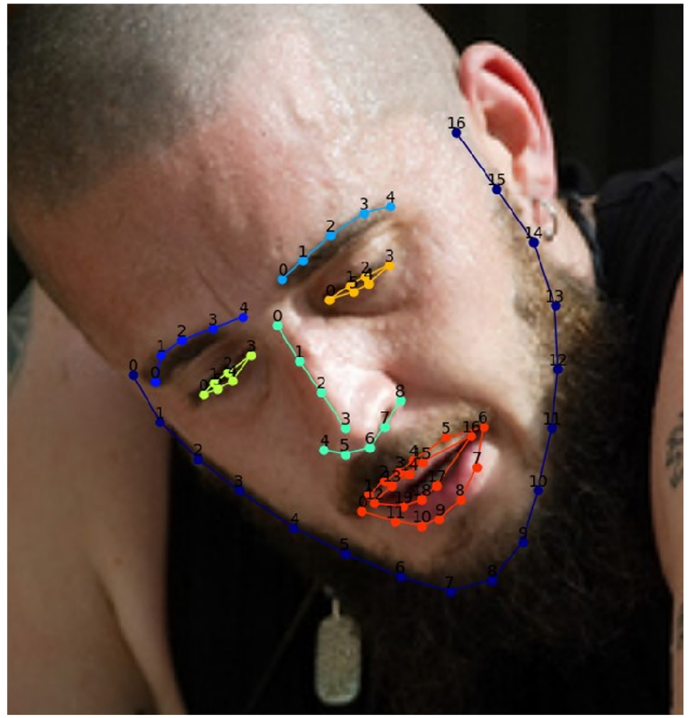
\includegraphics[width=0.6\linewidth]{dlib_landmarks}
	\caption{Facial landmarks are dependent of the face shape and morphology (image from \cite{dlib_review}).}
	\label{fig:2_dlib_landmarks}
\end{figure}


The intuition behind these methods are to \textit{project} the image of the face into a lower-dimensional space, which allows to extract significant features from each face. These features have to be consistent for the same face across different pose and lighting conditions (\autoref{fig:2_faces_poses}). An useful transformation when a dimensionality reduction is pursued is PCA (\textit{Principal Component Analysis}), a linear transformation that can be implemented to deal with the face recognition problem \cite{face_pca}.

\begin{figure}[h]
	\centering
	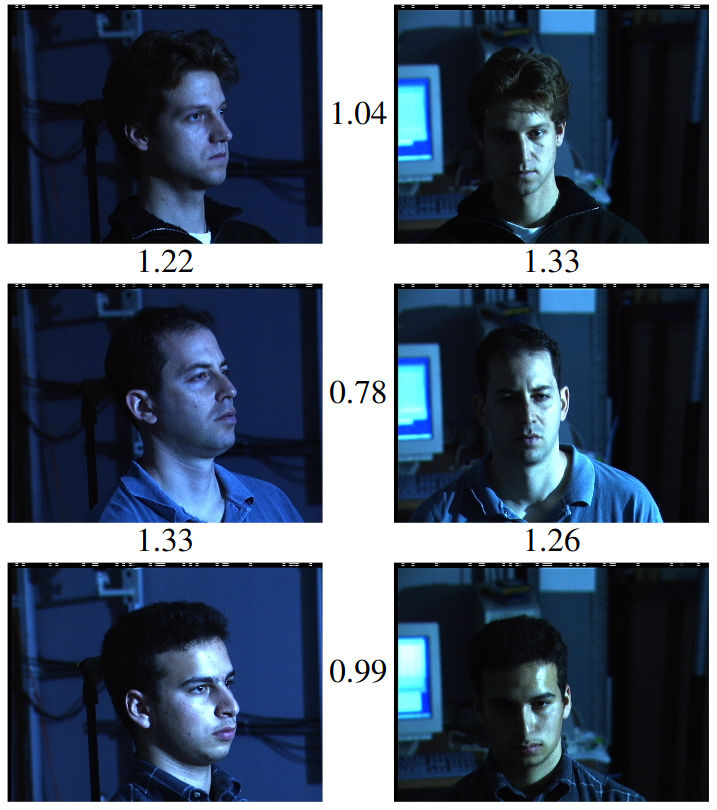
\includegraphics[width=0.40\linewidth]{face_poses}
	\caption{Examples of poses and light conditions across which the face projections are desired to be consistent for the same person (image from \cite{facenet}).}
	\label{fig:2_faces_poses}
\end{figure}
\vspace{4cm}
\subsection{Deep learning face identification: FaceNet}
\label{sec:2_facenet}
However, once again neural networks can be leveraged in order to achieve better performance: as the PCA is a linear operation, it could be learned by a single layer neural network. Thus, the introduction of deep networks can yield interesting results. The most relevant approach so far uses deep convolutional networks for performing this process \cite{facenet}, implementing an architecture called \textit{FaceNet}, which is partially based on the Inception \cite{inception} module, designed by Google researchers in order to greatly reduce the number of parameters in a neural network. What this network computes is called an \textit{embedding}, a projection of the input face image into a point in a 128-dimensional hyper-sphere. This allows to translate the identification into linear algebra terms, such as \textit{distance} between two faces, as well as clustering and applying unsupervised algorithms. The architecture can be visualized in \autoref{fig:2_facenet_architecture}. These networks can be trained using a loss function called \textit{triplet loss}, inspired by the work in \cite{lmnn_loss}. Given a training sample (\textit{anchor}), a \textit{positive} example (same class than the anchor) and a \textit{negative} example (different class than the anchor) are chosen, and the network is tuned to maximize the \textit{anchor-negative} embeddings distance, and minimize at the same time the \textit{anchor-positive} one (\autoref{fig:2_facenet_triplet_loss}).


\begin{figure}[h]
	\centering
	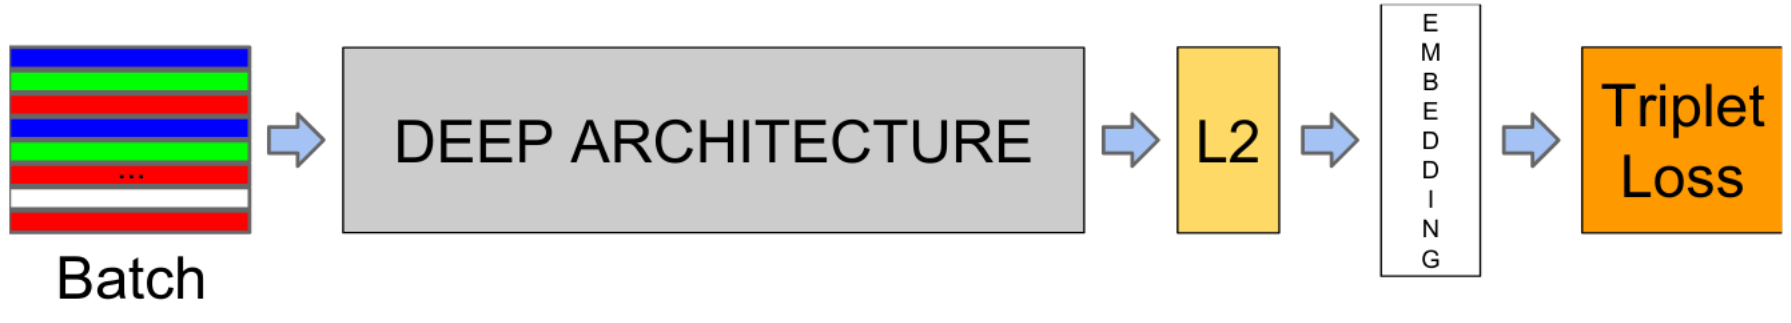
\includegraphics[width=0.7\linewidth]{facenet_architecture}
	\caption{Architecture of the FaceNet system (from \cite{facenet}).}
	\label{fig:2_facenet_architecture}
\end{figure}



\begin{figure}[h]
	\centering
	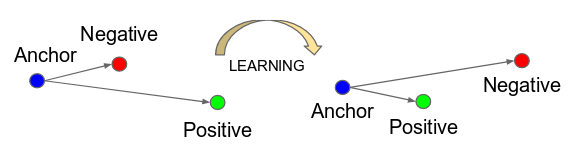
\includegraphics[width=0.7\linewidth]{facenet_triplet_loss}
	\caption{Triplet loss training. It minimizes the distance between an \emph{anchor} (current example) and a \emph{positive}, both of which have the same identity, and maximizes the distance between the \emph{anchor} and a \emph{negative} of a different identity (from \cite{facenet}).}
	\label{fig:2_facenet_triplet_loss}
\end{figure}


One thing to mention about the algorithms described above is that they perform the operations on the face image. Thus, a face detection is required for previously cropping the face of the person to be identified. One interesting approach using this technique is \textit{faced} \cite{faced}. This is a custom small ensemble of two neural networks, responsible to detect faces and correct the bounding boxes found. The main objective of the system is \textit{speed}, so the main detector architecture is based in YOLO \cite{yolov1}, and the second correction stage raises the precision achieved by the detector, achieving better results than a classical Haar approach, as illustrated on \autoref{fig:2_faced_vs_haar}. Further comparisons are performed on Chapter \ref{chap:4_results} between these two detection methods.

\begin{figure}[h]
	\centering
	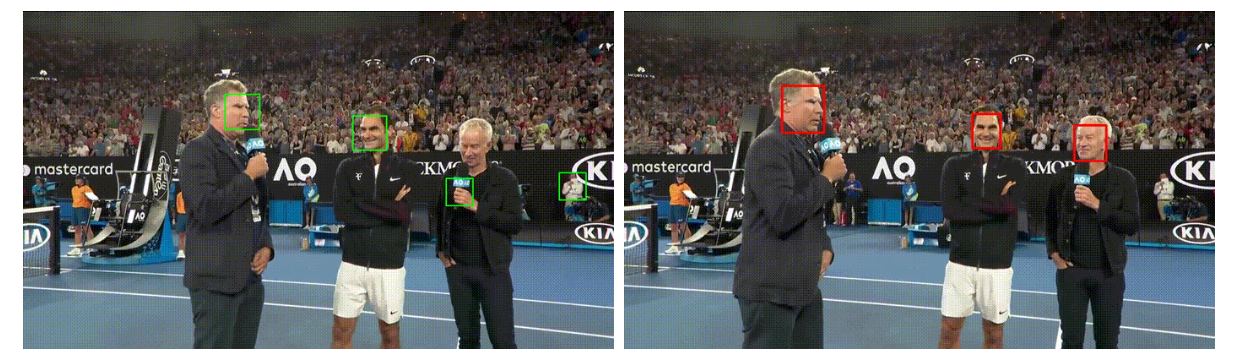
\includegraphics[width=0.8\linewidth]{faced_vs_haar}
	\caption{Classical Haar based face detector \cite{violajones} (left) vs. \textit{faced} (right). Image from \cite{faced}.}
	\label{fig:2_faced_vs_haar}
\end{figure}


\section{Embedded deployment}
\label{sec:2_embedded}
One of the requirements of this work is to be integrated in an autonomous robot. This imposes a power limitation on the algorithms to be deployed. Generally, the robotic systems are deployed using laptops connected to robots, as it was done in \cite{tfg} (\autoref{fig:2_real_tfg}).

\begin{figure}[h]
	\centering
	\begin{subfigure}[h]{0.4\linewidth}
		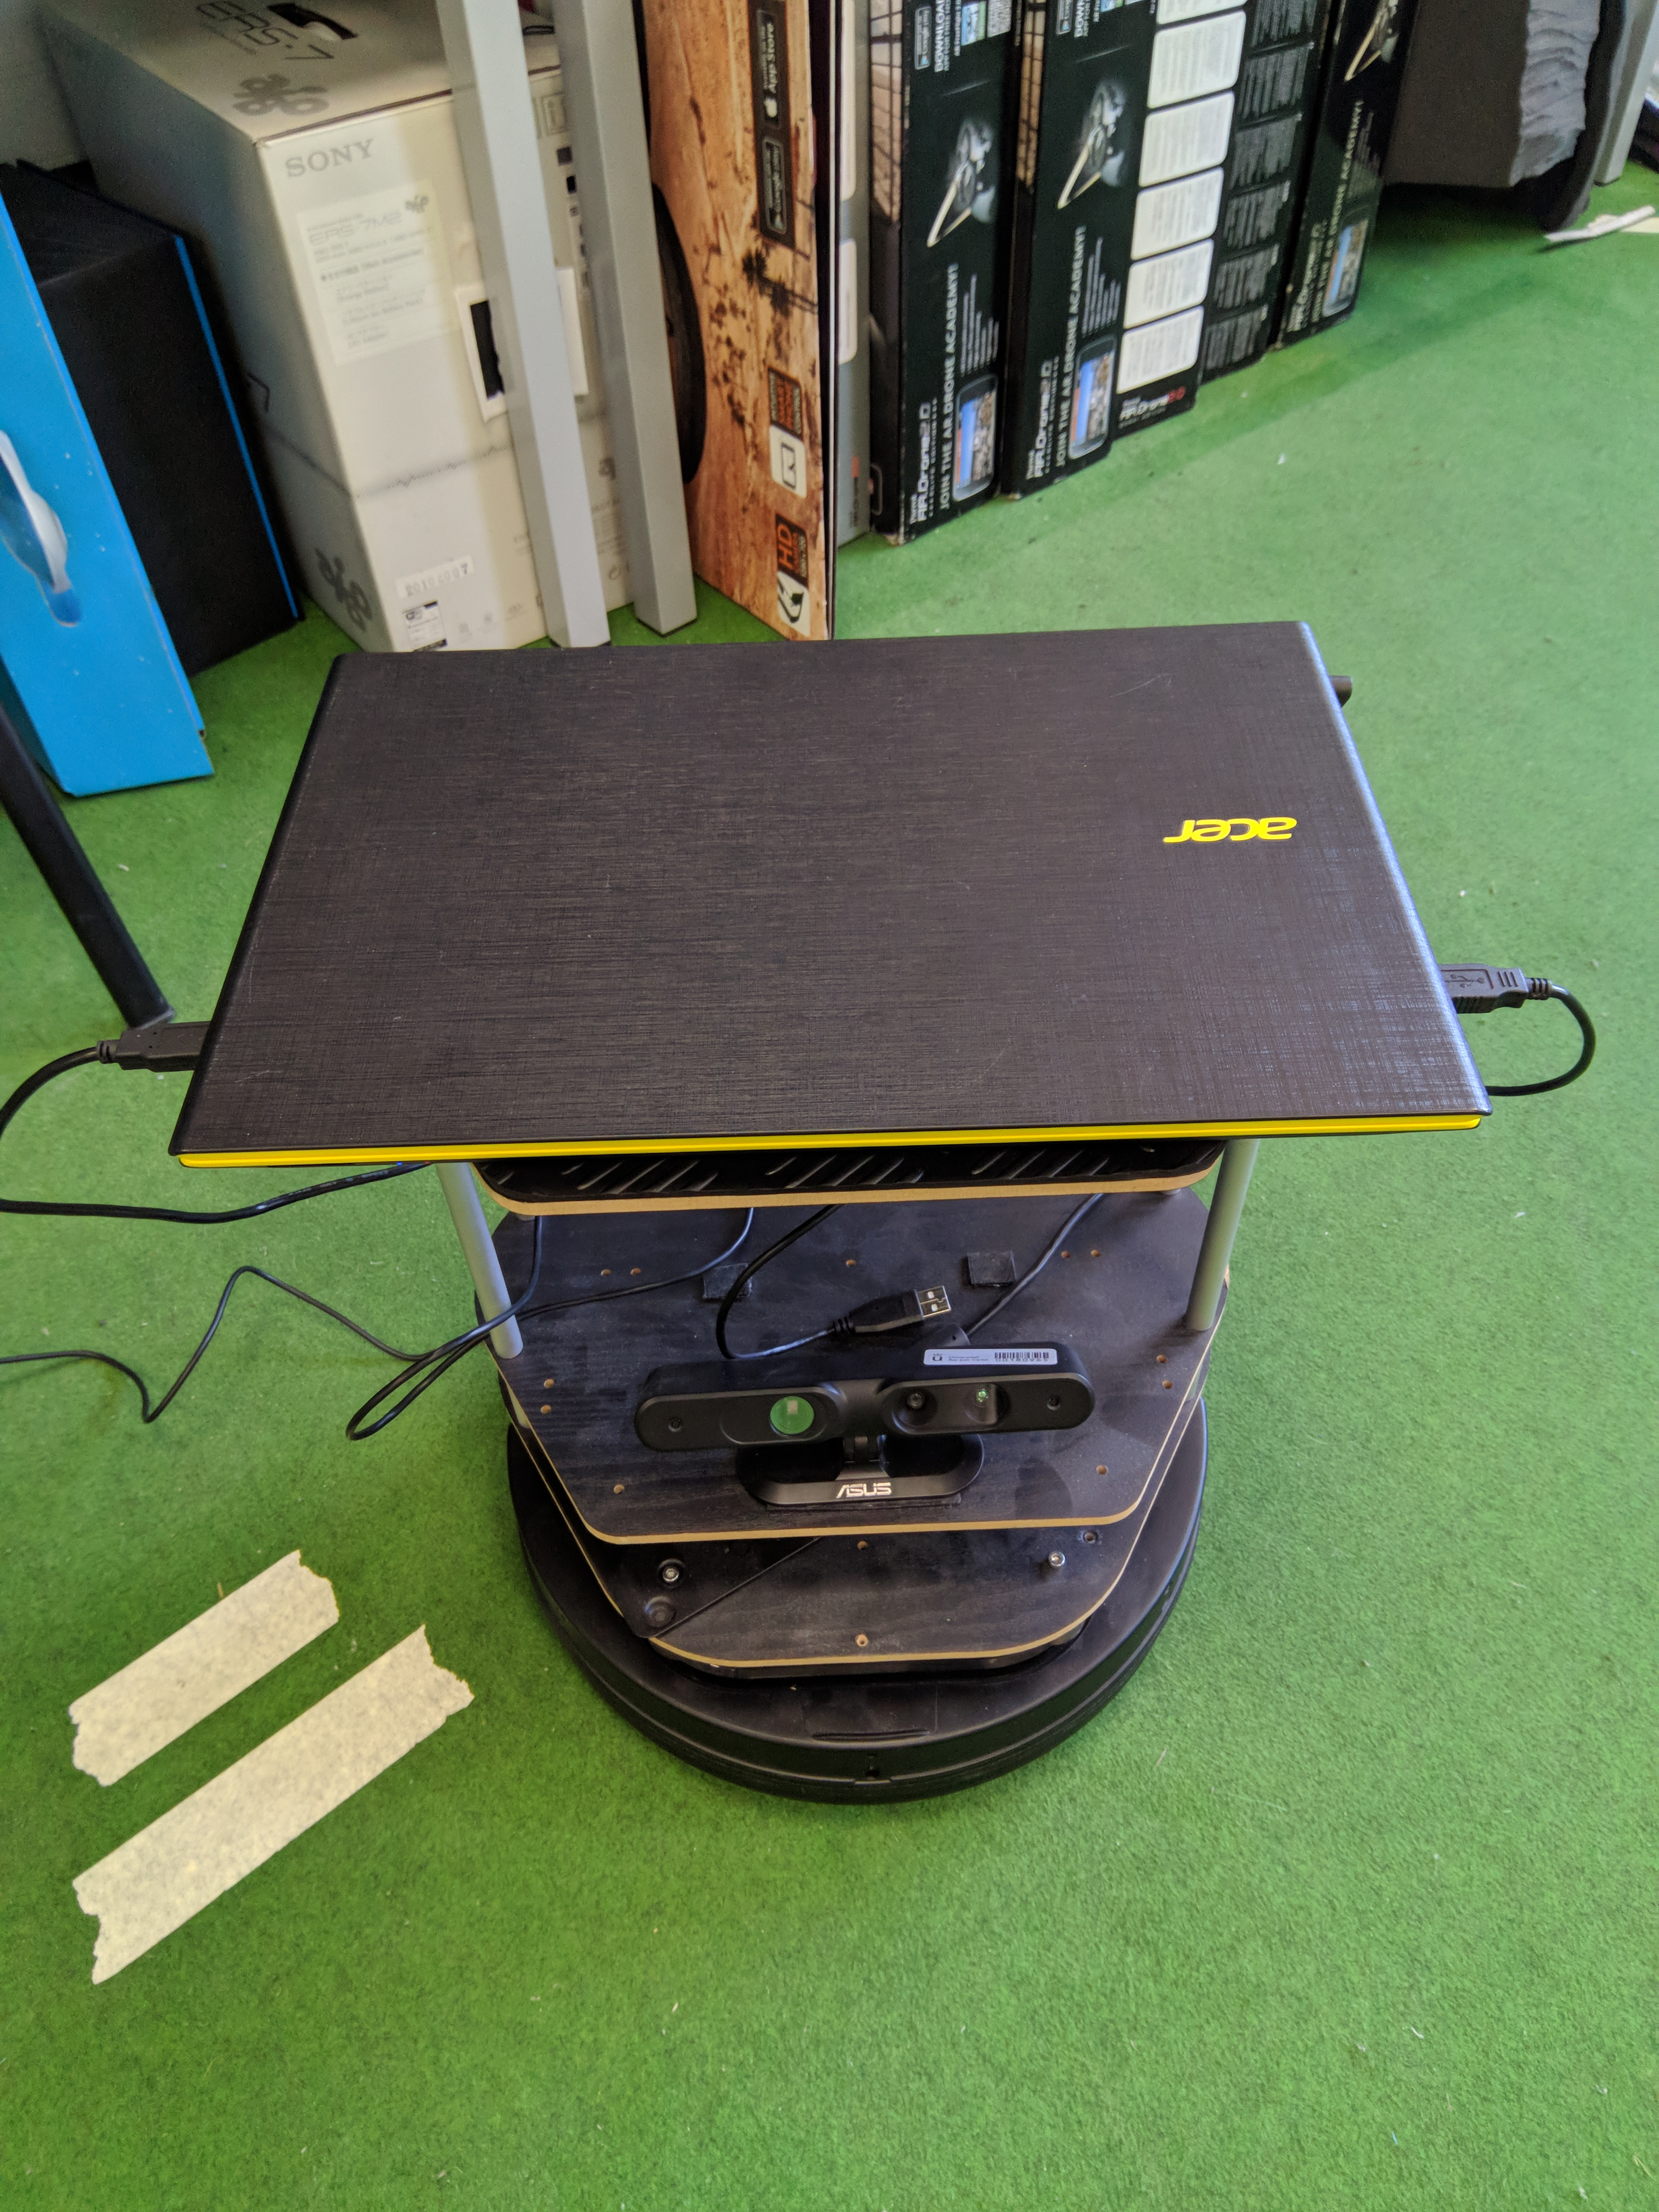
\includegraphics[width=1.9in]{tfg1}
		\caption{Frontal view.}
		\label{fig:2_turtlebot_front}
	\end{subfigure}
	\begin{subfigure}[h]{0.4\linewidth}
		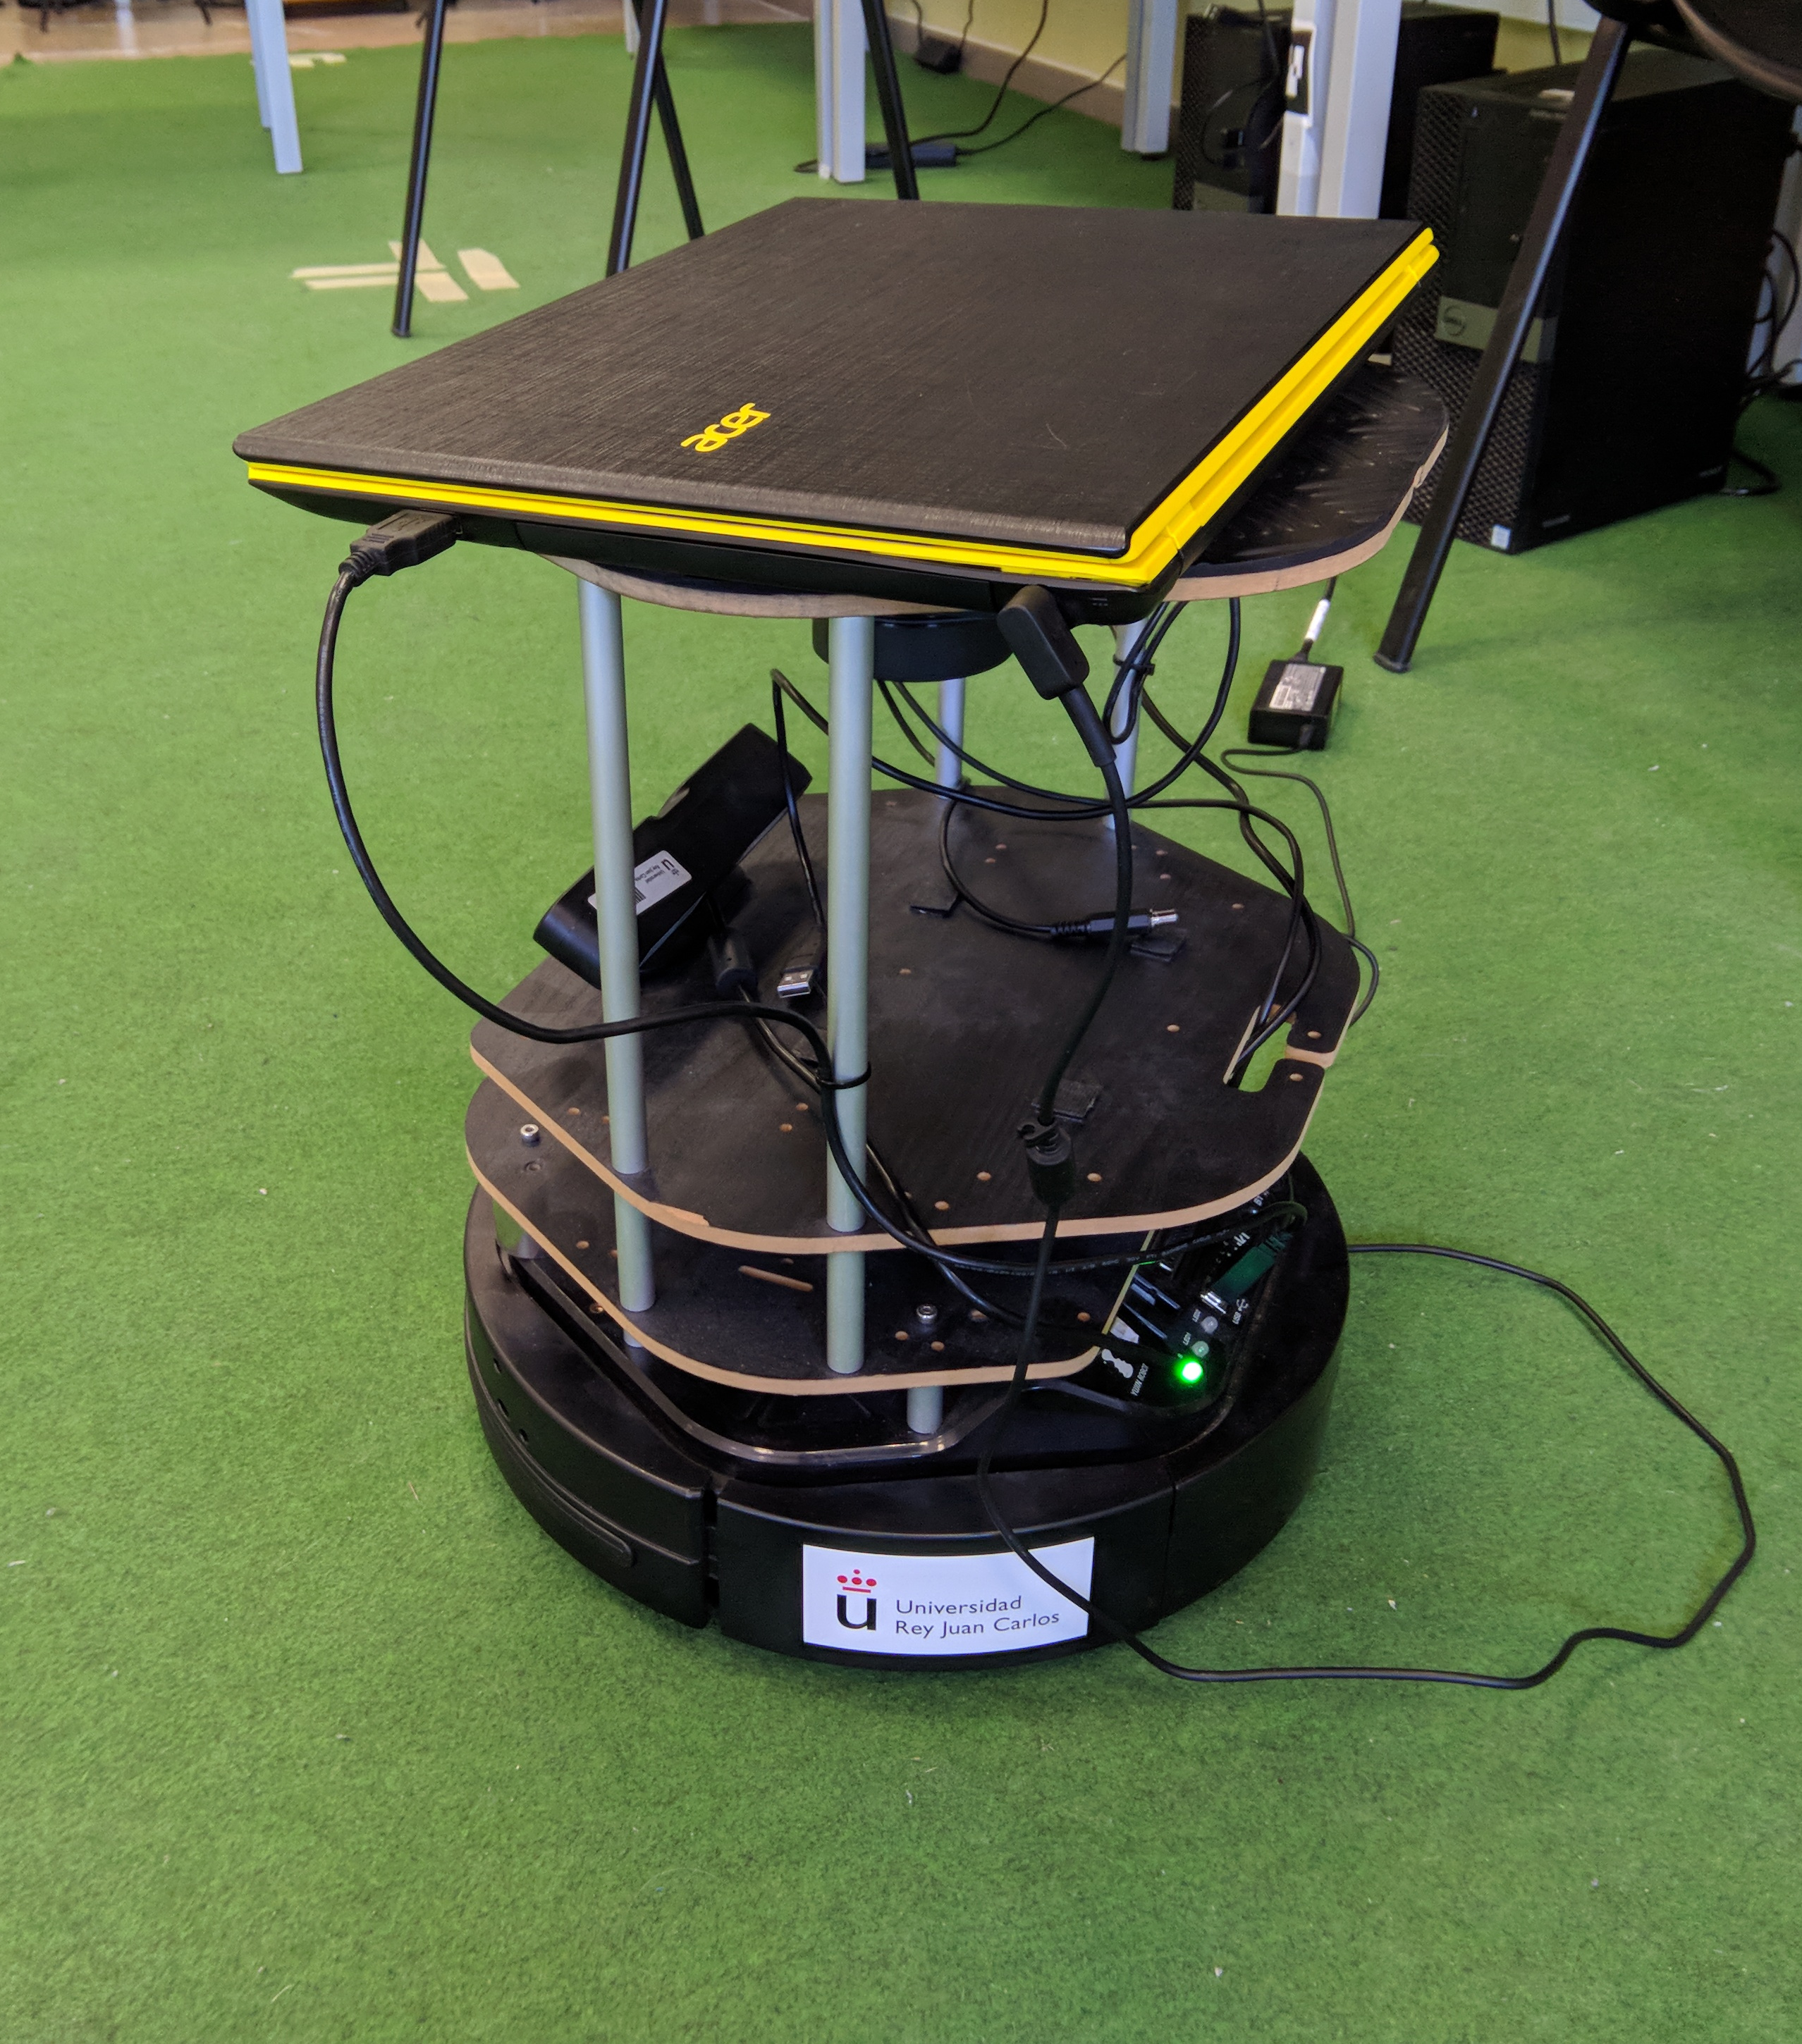
\includegraphics[width=2.2in]{tfg2}
		\caption{Side view.}
		\label{fig:2_turtlebot_side}
	\end{subfigure}
	\caption{Laptop+robot deployment on \cite{tfg}.}
	\label{fig:2_real_tfg}
\end{figure}

Nowadays, the mentioned increase in the interest into the real-time computer vision applications has fostered the development of specific low-power embedded devices to be integrated in mobile systems. The extending usage of devices such as Arduino or Raspberry Pi has led to embedded robotics systems, such as PiBot \cite{pibot} (\autoref{fig:2_pibot}). These robots are useful in the educational scope, as they are capable of running simple vision and navigation algorithms at a low cost.\\
\begin{figure}[h]
	\centering
	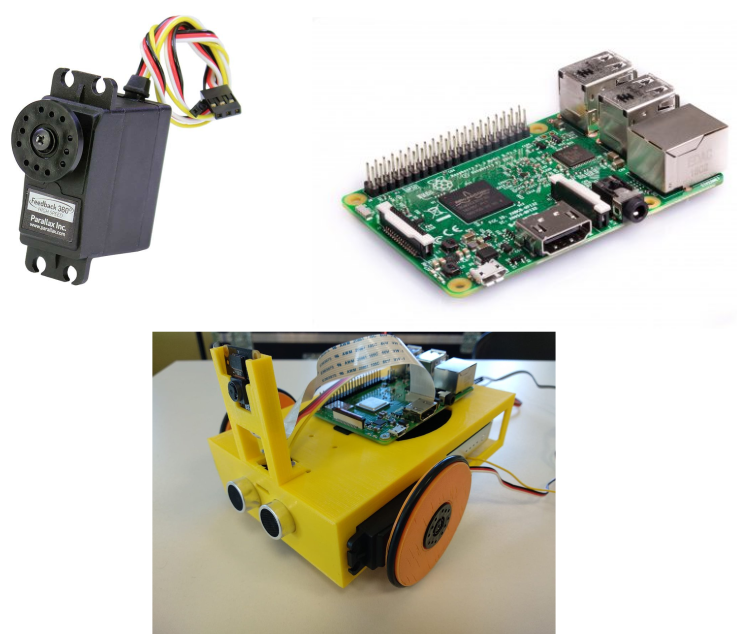
\includegraphics[width=0.5\linewidth]{pibot}
	\caption{PiBot, an open low-cost robotic platform for education (image from \cite{pibot}).}
	\label{fig:2_pibot}
\end{figure}
Unfortunately, the requirements for running more complex algorithms, such as neural networks, require of the next tier in power terms, keeping the portability nevertheless. The ideal device could be an ASIC (\textit{Application-Specific Integrated Circuit}), as the custom design would lead to a very tight optimization of the performance. However, the objective is to run the algorithms on existing software frameworks, requiring to use general purpose computers instead. The most remarkable advance in this scope are the Jetson devices manufactured by NVIDIA. These development boards are SoM computers running a tailored version of Linux. The fundamental feature of these systems is that they include a high-performance GPU featuring CUDA, a low-level parallel computation library, as well as several toolkits (such as TensorRT\footnote{\url{https://developer.nvidia.com/tensorrt}}) designed to optimize as much as possible the software implementations for the plethora of possibilities to be designed on this board. As it can be seen in \autoref{fig:2_tx2}, its size and power consumption make this system a good choice to be included in an autonomous robot. 
\begin{figure}[h!]
	\begin{subfigure}[h]{0.45\linewidth}
		\centering
		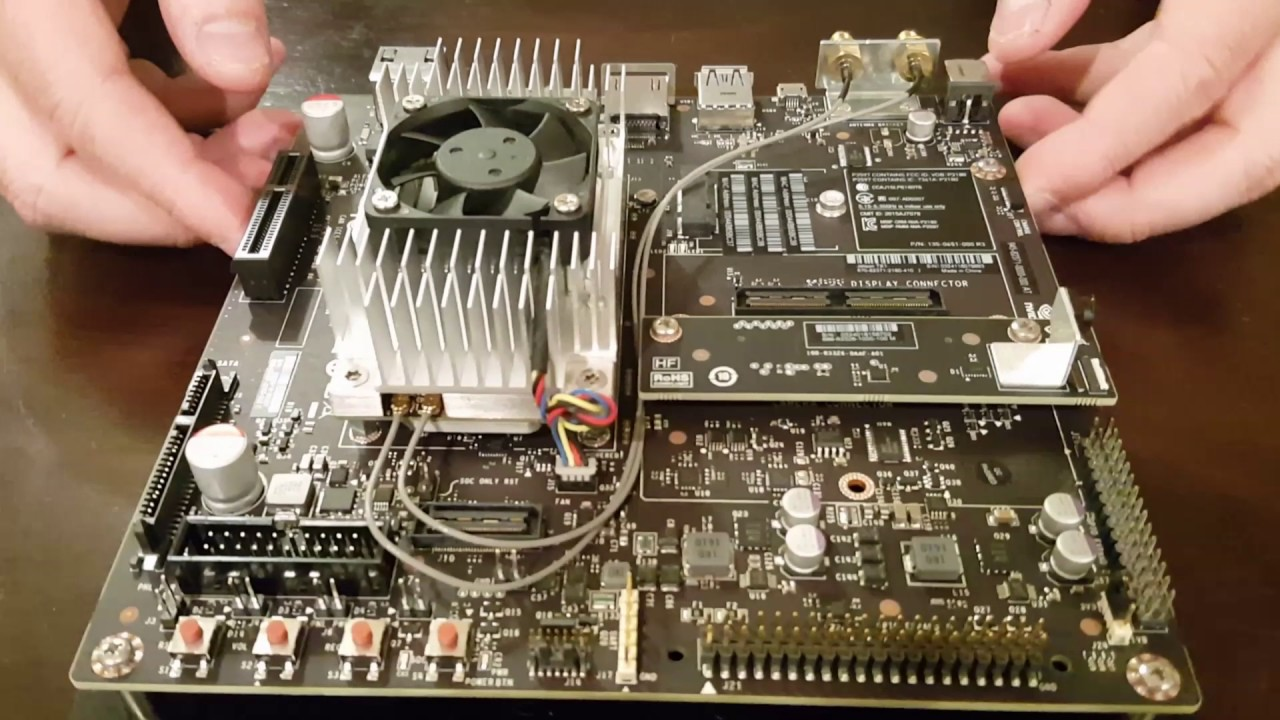
\includegraphics[width=\linewidth]{jetsontx2}

	\end{subfigure}
	\begin{subfigure}[h]{0.45\linewidth}
		\centering
		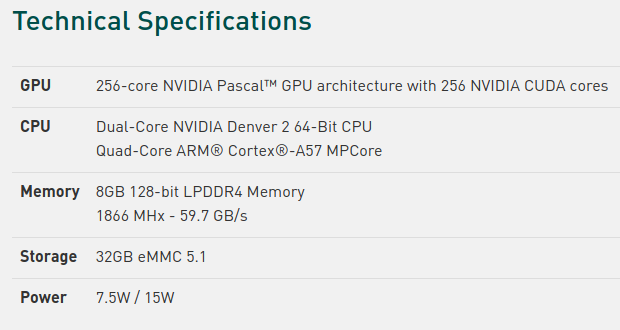
\includegraphics[width=\linewidth]{tx2_specs}
	\end{subfigure}
	\caption{NVIDIA Jetson TX2: an embedded high-performance device including a GPU.}
	\label{fig:2_tx2}
\end{figure}


\section{Person following}
\label{sec:2_following}
Several approaches have been developed pursuing this challenge of \textit{following a person}. Once the visual perception algorithms are established, the final output of the pipeline has to be a movement command for the robot to move towards the desired point. Mobile  robots can be classified according to their locomotion capabilities. A robot is \textit{holonomic} if the number of its controllable degrees of freedom is equal to its total degrees of freedom. If the controllable degrees of freedom are lower than the total degrees of freedom, the robot is \textit{non-holonomic}. This difference can be observed on \autoref{fig:2_holonomics}. In the case of a holonomic robot, the navigation process is simplified, as the robot can instantaneously move to a desired target. However, a non-holonomic robot needs to perform maneuvers in order to move towards a point.\\


\begin{figure}[h]
	\centering
	\begin{subfigure}[t]{0.45\linewidth}
		\centering
		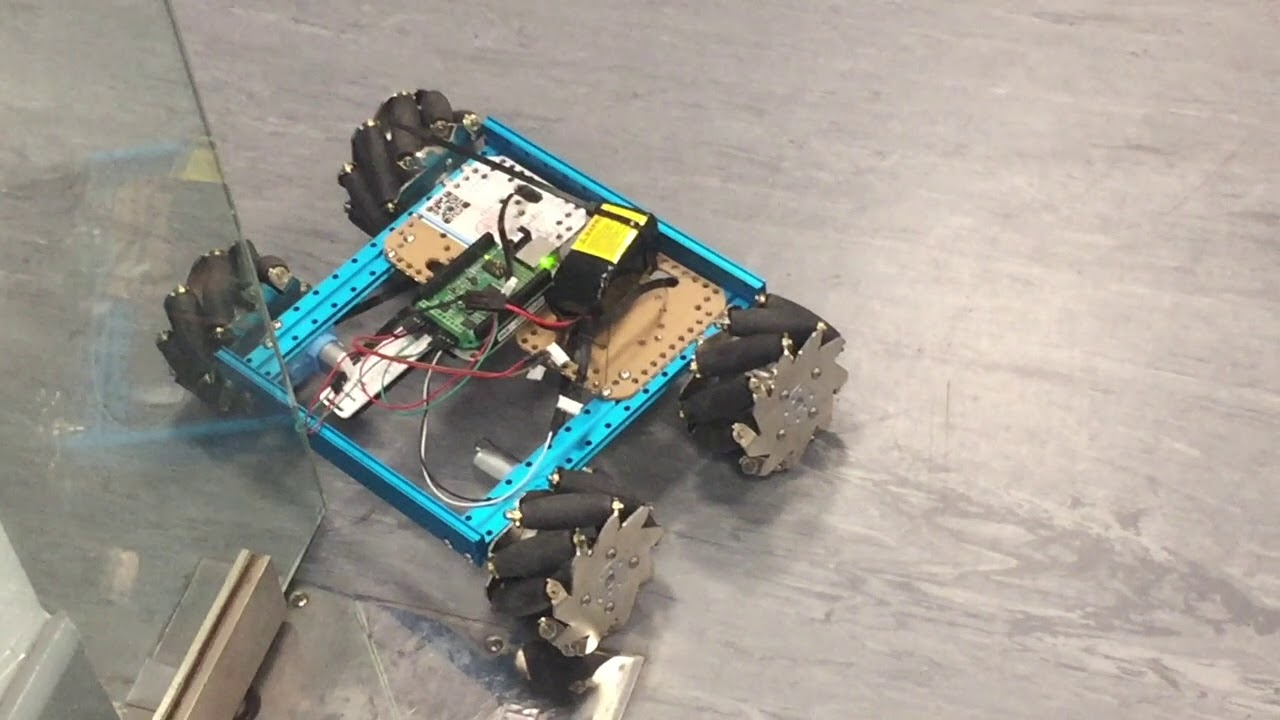
\includegraphics[width=\linewidth]{holonomic_robot}
		\caption{Holonomic robot.}
	\end{subfigure}
	\begin{subfigure}[t]{0.45\linewidth}
	\centering
	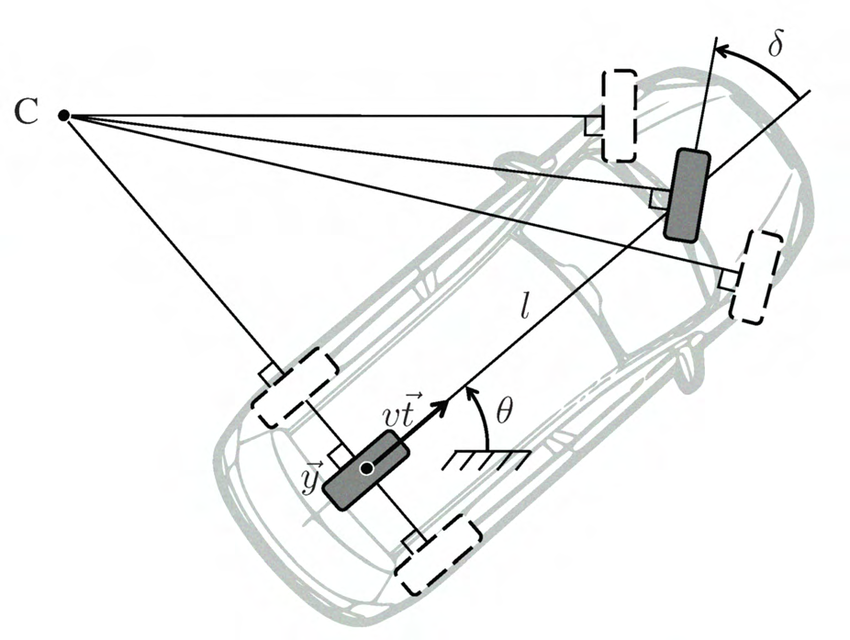
\includegraphics[width=\linewidth]{non_holonomic_robot}
	\caption{Schematic of the degrees of freedom of a non-holonomic vehicle (a standard car).}
	\end{subfigure}
	\caption{Comparison of a holonomic system with a non-holonomic one.}
	\label{fig:2_holonomics}
\end{figure}

The summary on \cite{personfollowing_summary} shows an interesting classification of some existing person following algorithms and their applications (\autoref{fig:2_personfollowing_summary}).


\begin{figure}[h]
	\centering
	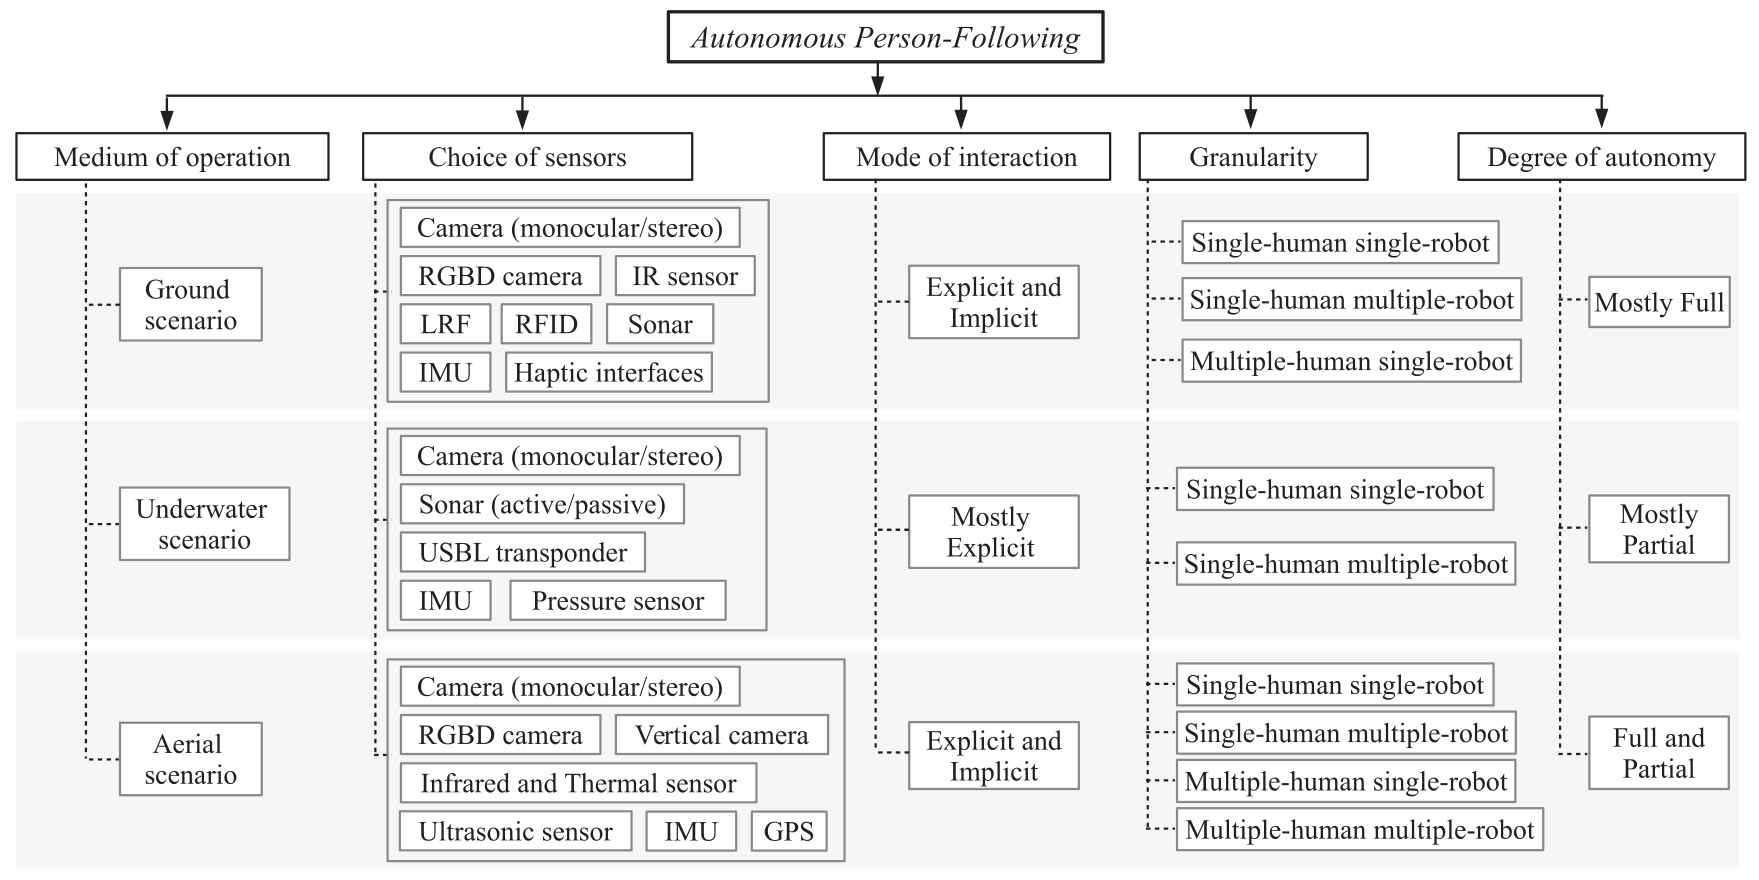
\includegraphics[width=\linewidth]{personfollowing_summary}
	\caption{In-depth classification of the existing person following algorithms (image from \cite{personfollowing_summary}).}
	\label{fig:2_personfollowing_summary}
\end{figure}

Some approaches leverage the detected objects in order to estimate the relative homography of the orthogonal planes, which allows to partially know the environment of the robot and trace a safe path towards the person, as it can be seen on \autoref{fig:2_personfollowing_homography}.

\begin{figure}
	\centering
	\begin{subfigure}[t]{0.45\linewidth}
		\centering
		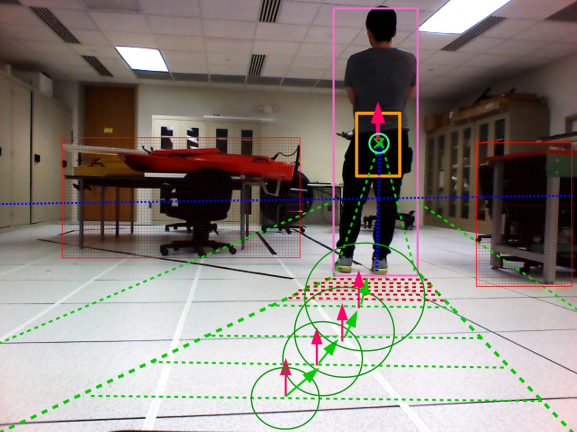
\includegraphics[width=0.95\linewidth]{personfollowing_homography}
		\caption{Following with path computation using homographies (image from \cite{personfollowing_summary}).}
		\label{fig:2_personfollowing_homography}
	\end{subfigure}
	\begin{subfigure}[t]{0.45\linewidth}
		\centering
		
		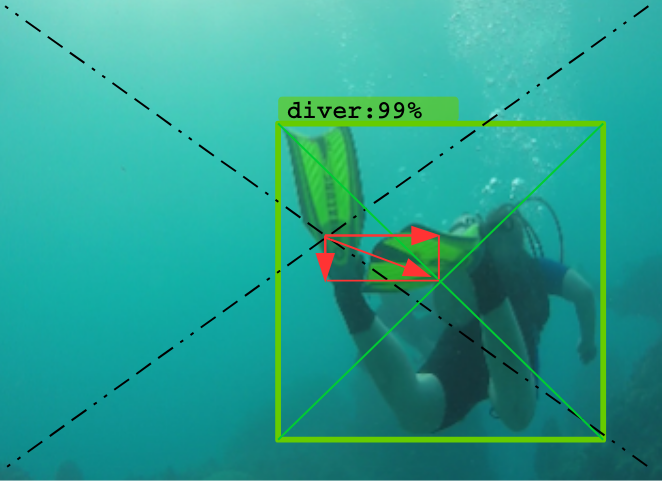
\includegraphics[width=0.95\linewidth]{personfollowing_reactive}
		\caption{Example of underwater reactive following (image from \cite{personfollowing_reactive}).}
		\label{fig:2_personfollowing_reactive}
	\end{subfigure}
	\caption{Examples of robotic following behavior.}
	\label{fig:2_personfollowing}
\end{figure}



Other approaches act without a path planning component, implementing what is called a \textit{reactive} behavior \cite{personfollowing_reactive}, similar to the proposed solution  on this work. On these approaches, the vector between the center of the image and the center of the person is used to command movements on the robot, as it can be seen on \autoref{fig:2_personfollowing_reactive}.

\newgeometry{voffset=-1.7cm,bottom=-0.1cm,textwidth=15cm}
\chapter{Materials and Methods}
\label{chap:3_materials_methods}
This chapter is devoted to describe the developed system. The development strategy was based in splitting up the functionality into different modules, which have been tackled sequentially. The next sections will cover each one of the modules, and will describe the achieved solution. Finally, the full ensemble will be described and tested.



\section{Available materials}
\label{sec:3_materials}
\subsection{Hardware}
\label{sec:3_hw}
\subsubsection{Base board}
As it was described in Chapter \ref{chap:2_sota}, typical following behaviors work on a personal computer attached to a robot. However, our solution is developed using a devoted SoM: the NVIDIA Jetson TX2, similar to the one described in \autoref{fig:2_tx2}. This system features a high-performance GPU, and low-level optimization engines, which greatly reduce the time required to perform the operations required for deep learning applications, such as tensor convolutions. The low power consumption of this board (15W at full power) makes it suitable to be embedded in a portable robot equipped with a battery. One drawback of this system is the scarce storage space. However, this can be immediately solved by installing an external storage device using its integrated SATA connector. In this project, a 120 GB Kingston SSD (\textit{Solid State Drive}) was used for this purpose, leveraging as well on the high transference throughput this device can achieve. It features a 64-bit ARM processor, and it mounts a fully functional Linux system. As it is equipped with two WiFi antennas, a remote control interface can be easily set using SSH connections. Regarding the available RAM in the board, it is limited to 8 GB, to be shared by the GPU and the CPU. This jeopardizes the execution of the deployed software and the neural networks, which have to be controlled in every moment in order to save the maximum amount of RAM possible. The resulting board can be visualized on \autoref{fig:3_mytx2}.\\

\begin{figure}[h]
	\begin{subfigure}[h]{0.35\linewidth}
		\centering
		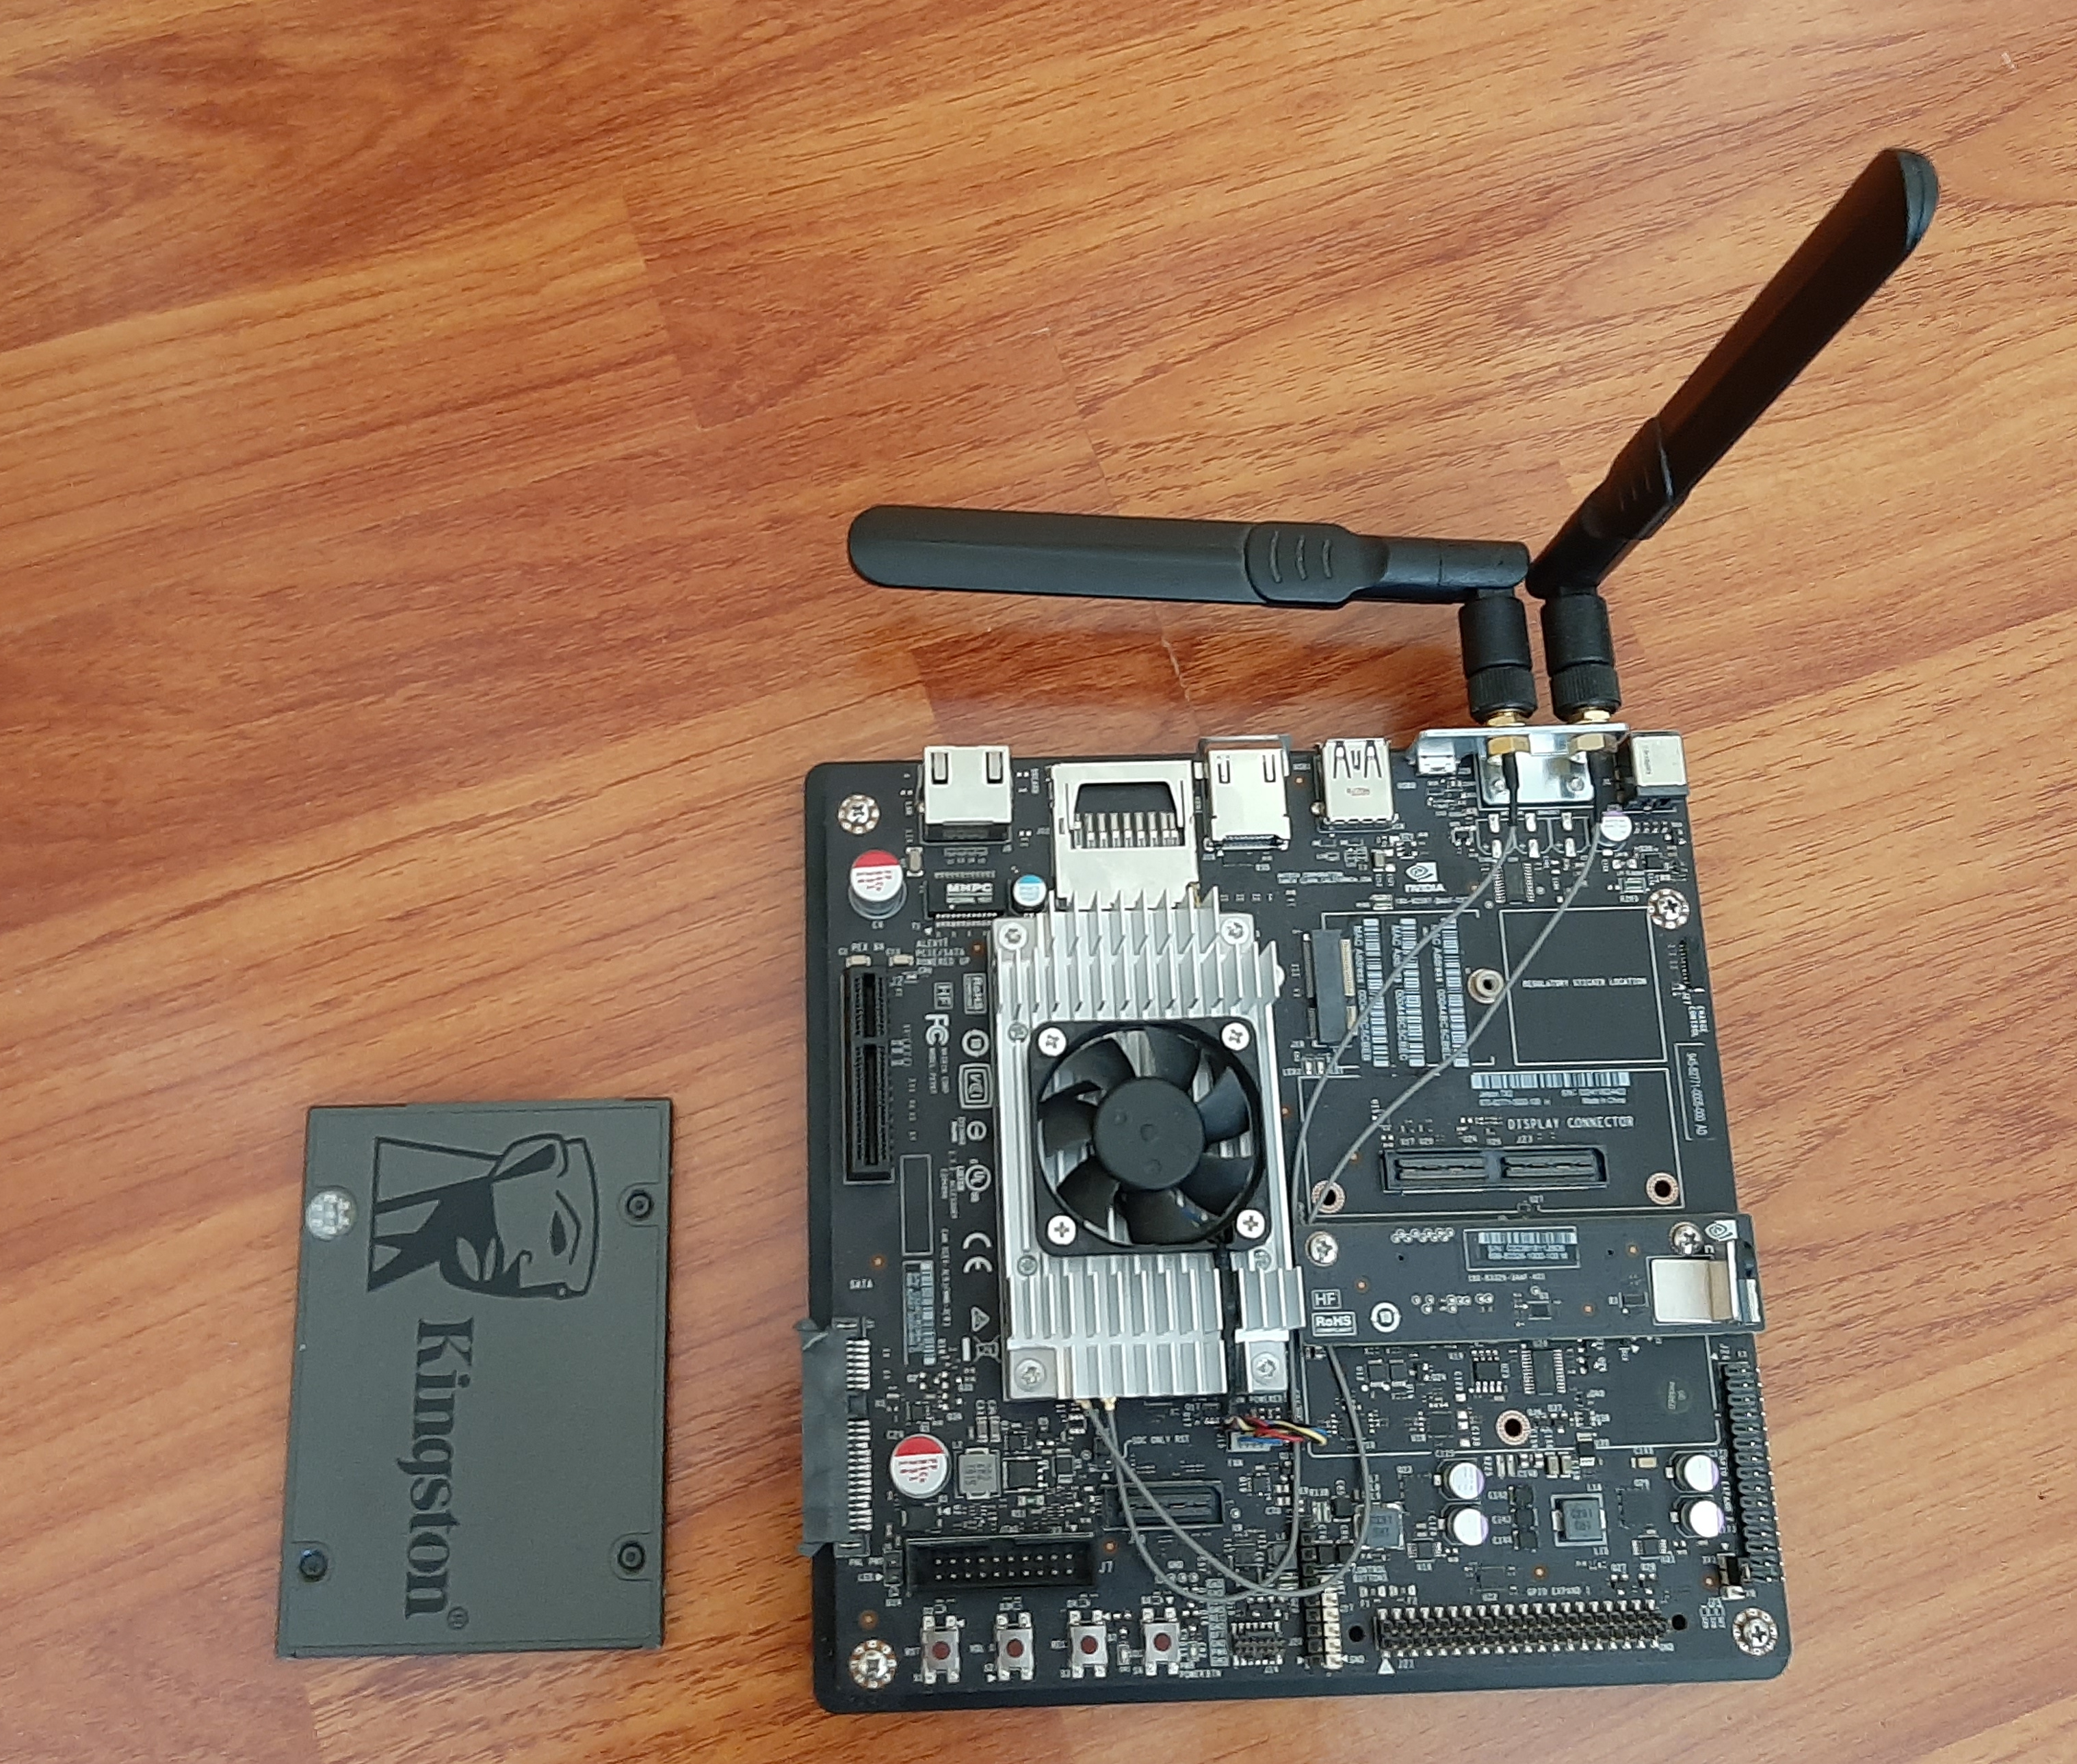
\includegraphics[width=0.98\linewidth]{tx2_nossd}
	\end{subfigure}
	\begin{subfigure}[h]{0.35\linewidth}
		\centering
		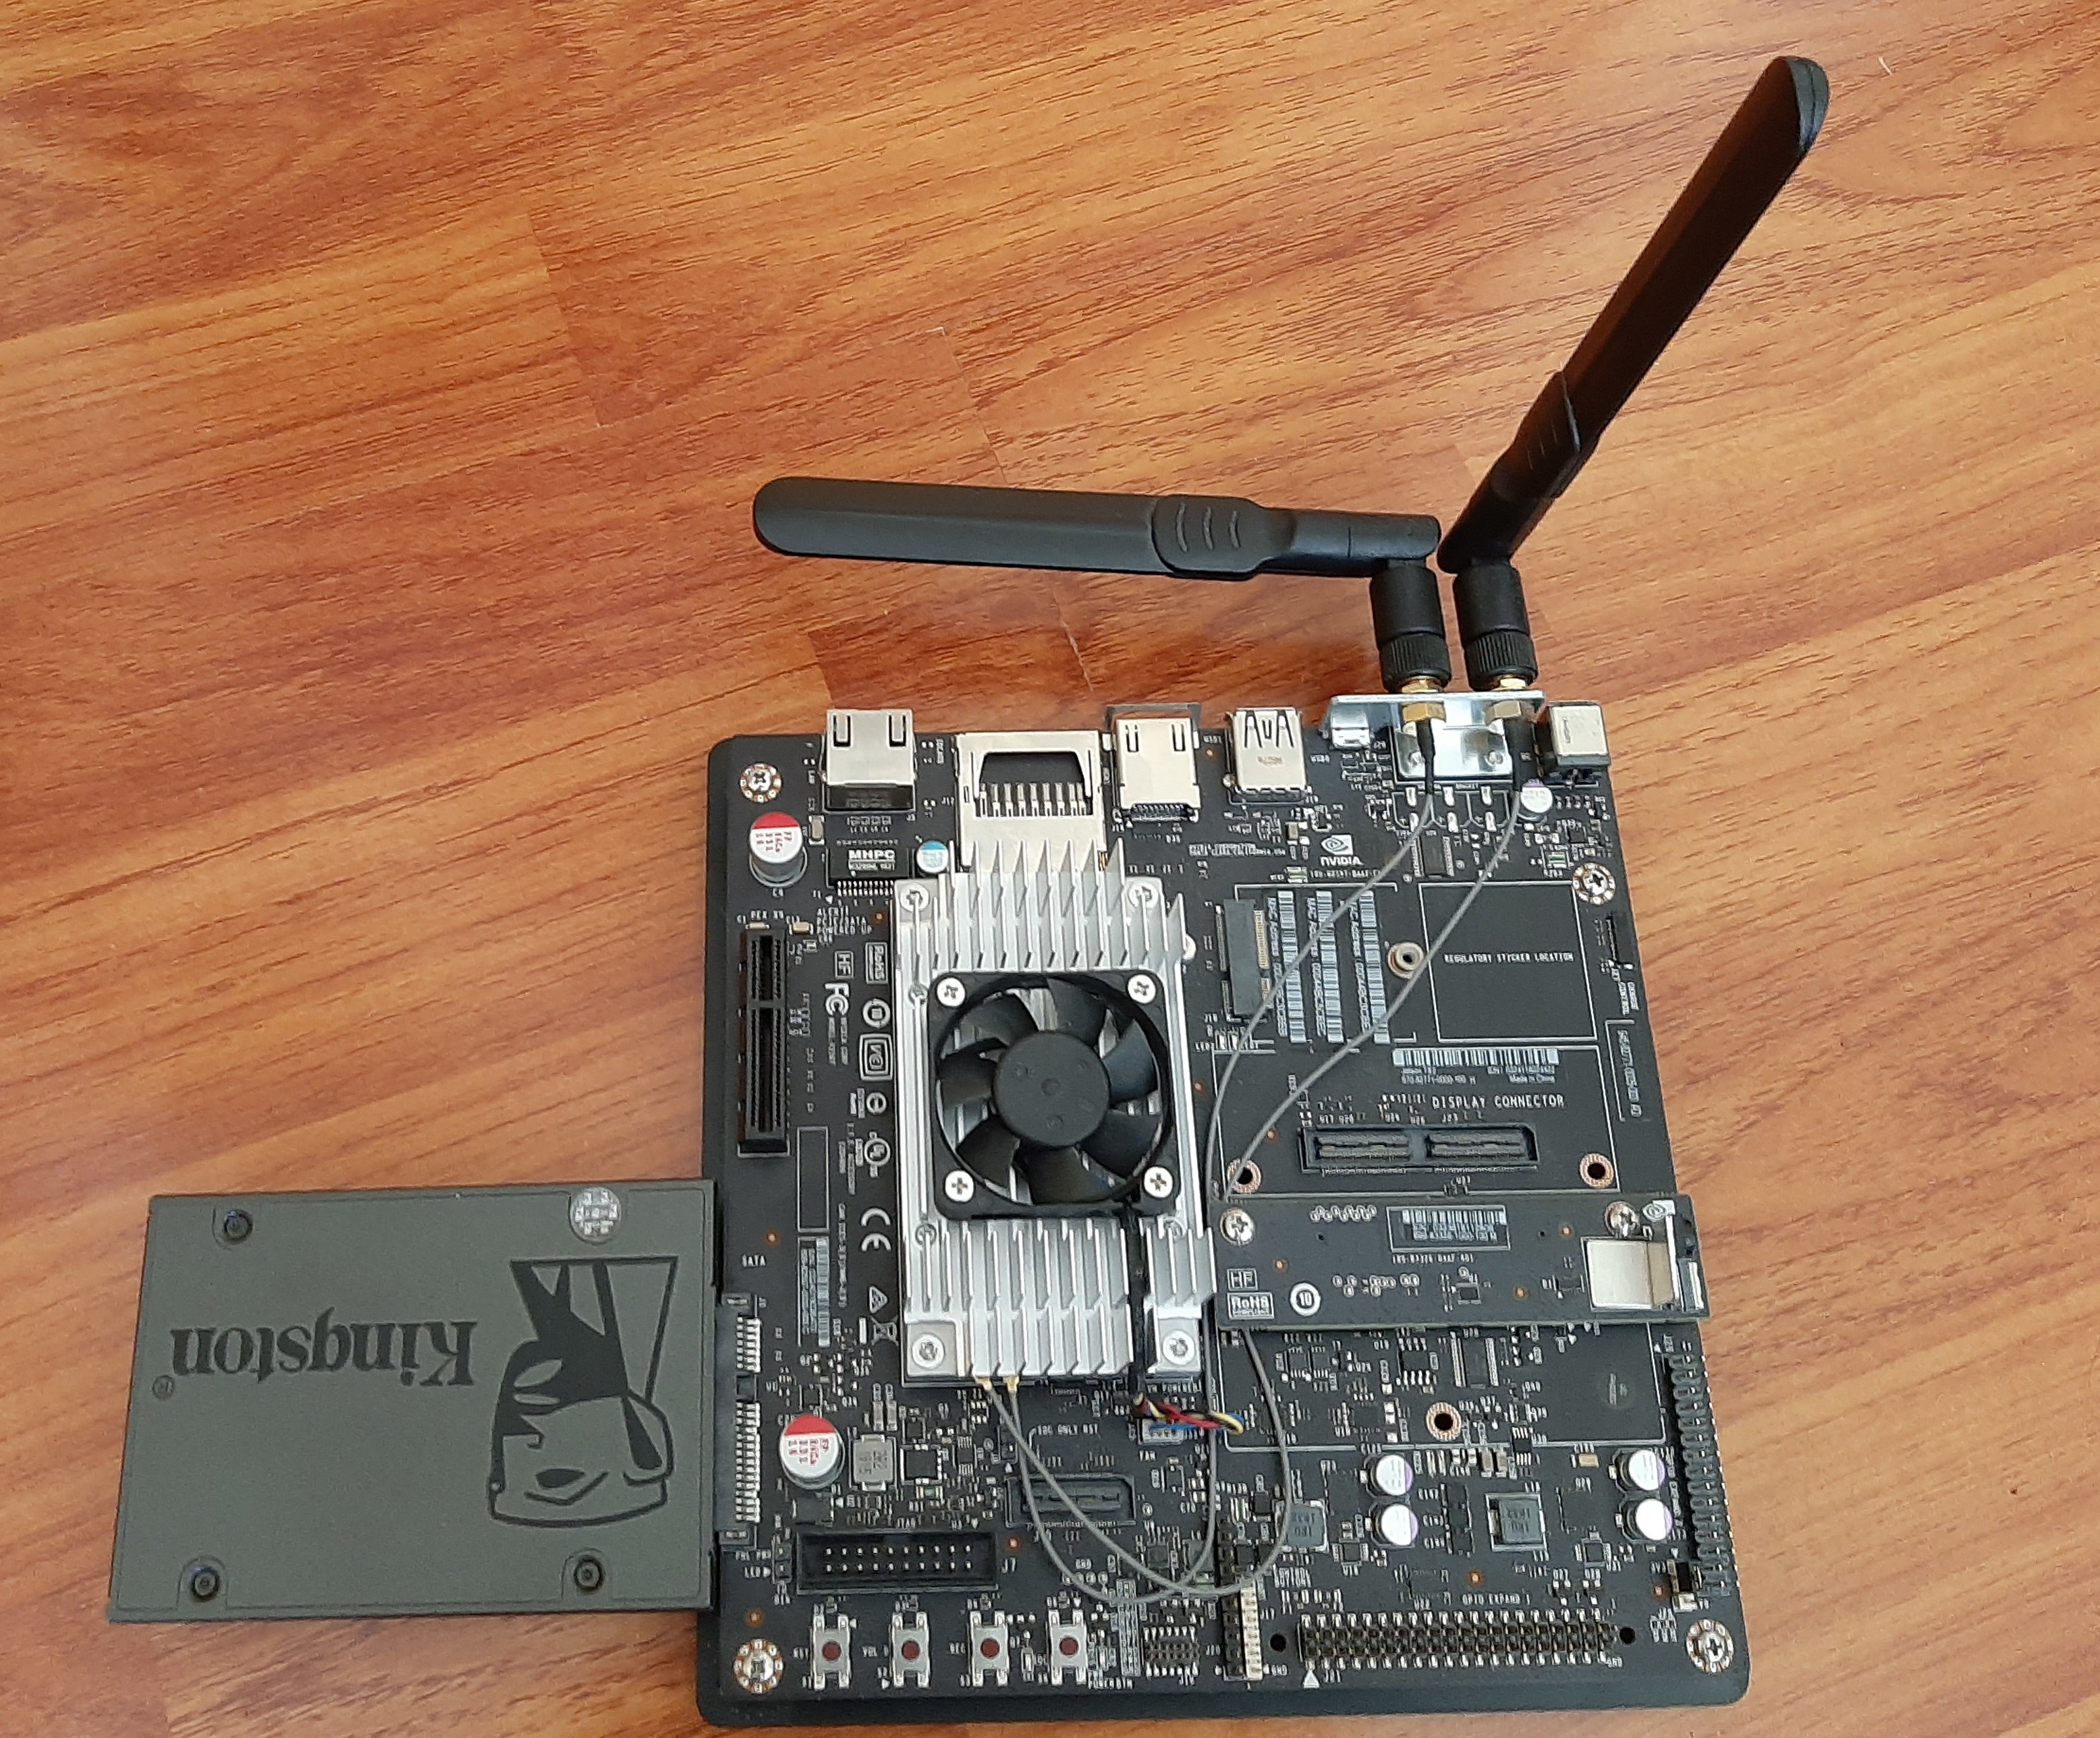
\includegraphics[width=\linewidth]{tx2_ssd}
	\end{subfigure}
	\caption{Resulting system: Jetson TX2 board and the installed SSD drive, plugged into the SATA connector.}
	\label{fig:3_mytx2}
\end{figure}
\vspace{8cm}
\restoregeometry

\subsubsection{RGBD sensor}

The vision system used in this work, the ASUS Xtion Pro Live (\autoref{fig:3_xtion}), is a USB device composed by a RGB camera and an IR (\textit{Infra-Red}) emitter + sensor system, capable of retrieving depth data for each pixel on the image. This is achieved by emitting a known light pattern (\autoref{fig:3_xtion_pattern}), which reflects in the present surfaces on the scene. These reflections are captured by the IR sensor, inferring the position of the surfaces from the received distribution of the IR pattern.

\begin{figure}[h]
	\centering
	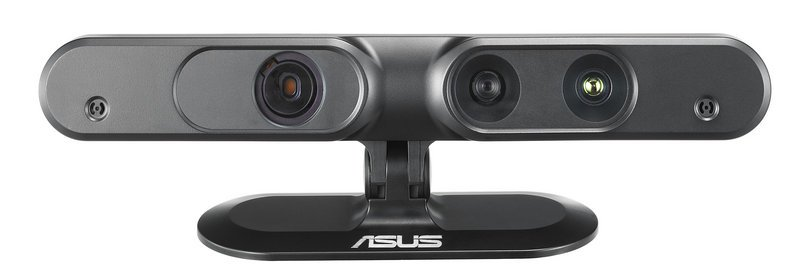
\includegraphics[width=\linewidth]{xtion}
	\caption{ASUS Xtion Pro Live}
	\label{fig:3_xtion}
\end{figure}

\begin{figure}[h]
	\centering
	\includegraphics[width=0.9\linewidth]{xtion_pattern}
	\caption{Infrared pattern emitted by the Xtion (images from \cite{rgbd_poses}).}
	\label{fig:3_xtion_pattern}
\end{figure}

The last problem to be tackled by this device is the discrepancy caused by the different points of view of the RGB and depth sensor. However, as the distance between these two sensors is fixed and known, a \textit{registration} process can be carried on inside the device, projecting the depth data into the RGB pixels \cite{diapos_cv_registration}.\\

\begin{figure}[h]
	\centering
	\includegraphics[width=0.9\linewidth]{xtion_discrepancy}
	\caption{Discrepancy between the RGB and depth images (image from \cite{tfg}).}
	\label{fig:3_xtion_discrepancy}
\end{figure}

The systems which implement the described design are called RGBD sensors. These are suitable for robotics, as the yielded result is a point cloud, reflecting the distance from the camera for each pixel in the image. Using this, the device is capable of projecting the 2-dimensional RGB image into the 3D space by means of the depth data (\autoref{fig:3_rviz}).\\

\begin{figure}[h]
	\centering
	\includegraphics[width=\linewidth]{rviz}
	\caption{Visualization of the RGB image (bottom left) and the resulting point cloud projected into the 3D space (right).}
	\label{fig:3_rviz}
\end{figure}

\subsubsection{Robotic platform}
On the other hand, the robot used in this work is the Turtlebot2 educational set. It is based on a Yujinn Robotics Kobuki mobile base (\autoref{fig:3_kobuki}), which is a non-holonomic robot with 2 degrees of freedom: \textit{linear speed} and \textit{angular speed}.\\
\begin{figure}[h]
	\centering
	\begin{subfigure}[h]{0.4\linewidth}
		\centering
		\includegraphics[width=0.9\linewidth]{kobuki}
		\caption{Appearance of the mobile base robot.}
		\label{fig:3_kobuki_appearance}
	\end{subfigure}
\begin{subfigure}[h]{0.5\linewidth}
	\centering
	\includegraphics[width=0.9\linewidth]{kobuki_panel}
	\caption{Schematic of the connections panel of the Kobuki.}
	\label{fig:3_kobuki_panel}
\end{subfigure}
\caption{Kobuki mobile base, which carries the rest of the structure.}
\label{fig:3_kobuki}
\end{figure}

In the Turtlebot2 set, the mobile base has an attached structure, carrying the RGBD sensor and a platform where typically a computer can be placed. This platform is useful to mount the NVIDIA Jetson device on. Additionally, as it can be seen in \autoref{fig:3_kobuki_panel}, the Kobuki panel is equipped with a 12V output, yielding up to 1.5A, which in power terms can be translated to a maximum power of 18W. Since the TX2 board peak consumption is 15W, this connector is suitable to power the system up, with an additional power margin of 3W. A lookup in the Kobuki user guide \cite{kobuki_manual} allows to find the suitable Molex connector, which can then be attached to two-wire cable and a rounded connector. This provides the NVIDIA Jetson of a 12V DC supply, similar to what it would obtain from a power outlet with a transformer. As the power input is equipped with a DC voltage regulator, it accepts voltages from 5.5V to 19V (table 59 in \cite{tx2_manual}).\\

Hence, this is a successful approach to build an \textit{autonomous} system: powering the computing board from the batteries of the robot, with enough autonomy to be powered on for several hours. The amount of time strongly depends on the usage of the motors of the mobile base, which are the most consuming component of the ensemble.\\

The final hardware setup is displayed on \autoref{fig:3_setup}, where the described components are combined to build the autonomous setup capable of running high-complexity person following algorithms.\\

\begin{figure}[h]
	\centering
	\begin{subfigure}[h]{0.45\linewidth}
		\centering
		\includegraphics[width=0.9\linewidth]{setup_front}
		\caption{Front view.}
	\end{subfigure}
	\begin{subfigure}[h]{0.45\linewidth}
		\centering
		\includegraphics[width=0.9\linewidth]{setup_rear}
		\caption{Rear view.}
	\end{subfigure}
	\caption{Autonomous setup: Turtlebot2 + Jetson TX2 + ASUS Xtion Pro Live.}
	\label{fig:3_setup}
\end{figure}

\newpage
\subsection{Software}
\label{sec:3_sw}
\subsubsection{NVIDIA JetPack}
The development of our person following behavior has been tackled using exclusively open-source software. The Jetson computing board follows a tightly optimized embedded design guidelines. A tailored version of Ubuntu Linux, named NVIDIA JetPack, is developed and maintained by NVIDIA, and it is available for download and install as the board firmware. For the developed system, the version used is JetPack 4.2.2 (R32.2)\footnote{Details available on: \url{https://docs.nvidia.com/jetson/archives/jetpack-archived/jetpack-422/release-notes/index.html}}. This custom implementation includes low-level interfaces for implementing parallel computing operations (CUDA), and several optimizations SDKs (\textit{Software Development Kits}), such as TensorRT. This engine is of special interest for us, as it allows to optimize the low-level implementation of a neural network, swapping certain modules (such as a convolution operation, a ReLU, or an Inception block), for a low-level optimized version of that module, allowing to greatly increase the inference speed without losing precision. More details about these optimizations will be explained later.\\

\subsubsection{Python}

This work has been developed using the Python programming language. In the previous work \cite{tfg}, the used version of the language was Python 2.7. However, as of today, that version has reached its EOL (\textit{End of Life}) date, remaining unsupported. For avoiding the obsolescence, all the code base was migrated to Python 3.6, a currently supported release, before making any change or improvement in the functionality.

\subsubsection{NumPy}

NumPy\footnote{\url{http://www.numpy.org/}} (\emph{Numeric Python}) is a library for Python (written in C++), born to extend the numerical capabilities of this language. It provides a powerful \texttt{ndarray} class, which allows to keep an N-dimensional collection of values/objects in a really handy way (in comparison with Python's standard \emph{lists}). It also provides a rich set of methods to manage arrays (such as advanced indexing, shaping, data formatting, etc.).\\


These capabilities immediately turn this library into an excellent framework for data processing in a lower level. It allows to store and handle images and tensors on an intuitive way, providing methods to perform typical tasks such as row-wise/column-wise averaging, transposing, type conversion, or matrix slicing. The majority of these structures and methods are implemented using the C++ language, which provides a higher speed than a Python implementation.




\subsubsection{ROS}
This project requires hardware-software interaction, as the development board needs to read the images captured by the Xtion sensor, as well as sending the final velocity commands to the robot. For this purpose, the ROS middleware is used. ROS (\textit{Robot Operating System}) is ``\textit{an open-source, meta-operating system for your robot}'', maintained by the \emph{OSRF} (\textit{Open Source Robotics Foundation}) \cite{ros-intro}. It is a framework that provides a distributed, easily-scalable environment of \emph{nodes}. These nodes are programs which run independently on the computer (or distributed over a network), so they can perform individual tasks. However, they can communicate between themselves on a synchronous way (over \emph{services}, implementing a client-server role system between nodes), or on an asynchronous way, via \textit{topics}. These topics, which rely on a standard TCP/UDP communication between sockets, are intended for an unidirectional, streaming communication, where a node can take roles: \emph{publisher} (if it is writing data inside the topic), or \emph{subscriber} (if it is reading the data that publishers are broadcasting into the topic). The data stream through the topic is not unrestricted, it must follow a ROS specific syntax, a \emph{Message} type, which is strictly defined for the communication purpose (geometry, sensoring, etc.).\\

For this project, the packages \texttt{cv\_bridge} and \texttt{openni2\_camera} have been used for handling the RGBD data. The robot can be controlled with the package \texttt{kobuki\_node}. All the software architecture is controlled by \texttt{rospy}, the interface for Python to communicate with the described ROS infrastructure.\\

Another useful feature of ROS middleware is the \textit{ROSBag} storage system. Recording a ROSBag allows to save in a single file the messages read from several topics for the time it is recorded. Later, the ROSBag can be played again to recover the messages from the topics, in the same order they were recorded. This is useful for recording video sequences from the RGBD camera, saving simultaneously the image and depth information, allowing the user to perform testing of different parameters using the exact same image source.\\

As well as in the Python case, the version of ROS used on \cite{tfg} reached its EOL date. Thus, the ROS version has been migrated as well to the currently supported release: \textit{Melodic Morenia}, which firstly provided the compatibility with Python 3. As the Jetson TX2 board is based on an ARM architecture, this upgrade has required several tweaks on the software compiling and implementation processes, which have been properly documented in the project repository\footnote{\url{https://github.com/RoboticsLabURJC/2017-tfg-nacho_condes}} for the sake of repeatability.\\


\subsubsection{OpenCV}
For general image processing, OpenCV (\emph{Open Source Computer Vision}) is a C++/Python/Java open-source library (natively written in C++) for Computer Vision purposes. Among the classic/\emph{state-of-the-art} methods it bundles, several functions can be found suitable for face recognition, image stitching, eye tracking, computing homographies, establishing markers for augmented reality, etc.\\

OpenCV focuses on \emph{efficiency and real-time functionality}, due to the low-level optimizations at hardware level (i.e., integration with NVIDIA CUDA and OpenCL GPU processing libraries). Thus, the excellent performance achieved by this open source library has turned it into the \emph{de facto} standard for every kind of users (from researchers to big companies or even governmental bodies, as their website stands\footnote{\url{https://opencv.org/}}).\\

This library has been used across the entire project, on its version number 4.2.  It has been useful for diverse tasks, such as image normalization, drawing, computing local features or optical flow approximations.



\subsubsection{TensorFlow}


The deep learning framework used is TensorFlow. This is a high-performance numerical computation library, strongly focused on parallel computing, typically carried on by GPUs or processing clusters. This library is a state-of-the-art tool to deploy deep neural networks because of its efficiency. Besides of training/running a neural model, this library allows to load a pretrained model from a storage device, by means of a \textit{frozen graph} file. This file contains both the network definition and the weights of its nodes.\\

Additionally, a binding component called \texttt{TensorFlowRT/TRT} have been used to implement the low-level optimizations on the TensorFlow neural engines, as it will be described later.


\newpage
\section{Design}
\label{sec:3_design}
The software implemented in this work has been divided into two main components or modules, namely the \textit{Perception} module and the \textit{Actuation module}, which can be observed in \autoref{fig:3_functional_architecture}.

\begin{figure}[h]
	\centering
	\includegraphics[width=0.7\linewidth]{functional_architecture}
	\caption{Functional architecture of the developed work, showing the two main blocks.}
	\label{fig:3_functional_architecture}
\end{figure}

These two modules cope with specific tasks on an independent manner, as it will be described in the following subsections.


\subsection{Perception Module}
\label{sec:3_perception}
This module encompasses what the robot perceives from its sensors (the camera, in this case), and the subsequent processing of the images in order to determine the location of the person to be followed.
\subsubsection{Camera}
As it was described before, the Xtion device yields two simultaneous images: an RGB image and a depth image. The ROS controller for the camera, OpenNI2\footnote{\url{https://structure.io/openni}}, fetches the image and registered depth map from the camera, making this information available through several ROS topics. As ROS follows a \textit{publisher-subscriber} semantics, once the driver is up and running, any application may subscribe to the topics in order to receive all the published messages. In our \textit{Camera} module, two subscribers are deployed to retrieve the latest \textit{(RGB, depth)} pair on an asynchronous way. These images are then converted into the standard image format in the OpenCV library, and they are ready to be used by other components. Additionally, in order to be able to perform objective testing and benchmarks, the Camera module is able to retrieve the images from a recorded ROSBag instead of the online camera. This is useful to obtain objective metrics of another components of the software on unit tests, as the ROSBag ensures that exactly the same images are used regardless the tested system.\\

The implemented \textit{Camera} module abstracts this condition, allowing to apply the system to an \textit{online} source (camera) or an \textit{offline} source (recorded ROSBag), with a transparent adaptation to the rest of the system. Whenever a new (RGB, depth) pair is required, the \textit{Camera} module will serve the latest available image from the specified source.\\


\subsubsection{Neural pipeline}

The captured images are passed through an ensemble of neural networks, which provide the capability of detecting the persons in the scene, as well as identifying which one is the one to be followed. As it was studied in Chapter \ref{chap:2_sota}, the most powerful and robust approaches are achieved nowadays using deep learning. Thus, the complex problem of determining the identity and location of the person of interest has been decomposed into three tasks, which are all addressed using the corresponding deep learning techniques:
\begin{enumerate}
	\item \textbf{Person detection:} the \textit{object detection} task (\autoref{fig:3_person_detection}) is a common one in computer vision. The existing solutions use object detectors similar to those explained in Chapter \ref{chap:2_sota}, which are typically trained with large image datasets. The classes these models are capable to detect contain the \textit{person} class. Thus, as it was demonstrated in \cite{tfg}, a deep object detector can be readily used for detecting persons. In this work, several models have been tested, varying the base network architecture and its depth. Since one of the objectives of the system is to work on a portable (low-power) system, only the architectures which yield a good performance with a sufficiently low inference time are considered. The two most suitable models for this purpose are SSD \cite{ssd} using a MobileNet \cite{mobilenet} for feature extraction, and the \textit{tiny} version\footnote{The usage of the tiny version of YOLOv3 is due to issues with the limited memory on the Jetson TX2 board. The full model was tried unsuccessfully, as it requires more memory than the available one on a typical execution.} of YOLOv3 \cite{yolov3}. These models are already trained and publicly available on the TensorFlow Model Zoo \cite{model_zoo} and on repositories hosted on GitHub\footnote{\url{https://github.com/mystic123/tensorflow-yolo-v3}}. In-depth tests have been conducted to compare the performance of these two models, which can be found in Chapter \ref{chap:4_results}. The previously developed work \cite{tfg} only supported SSD-based detectors, however, the object detection component of the program has been upgraded and it features YOLOv3 support as well, making it available through the configuration file specified on launch.
	
\begin{figure}[h]
	\centering
	\includegraphics[width=0.5\linewidth]{person_detection}
	\caption{Example of a person detection task.}
	\label{fig:3_person_detection}
\end{figure}
	
	\item \textbf{Face detection:} as the previous task, this problem can be addressed using an object detection neural network. However, the previously described models are not suitable for detecting faces, as that object class was not included among the labels on the datasets used for training the networks. In this case, the adopted solution is a single-class detection system. The network trained in \cite{faced} implements a two-stage neural network capable of detecting faces. As it was explained in Chapter \ref{chap:2_sota}, this detector is based on YOLO, which ensures a high-speed and efficient detection based on a class-specific neural network, which is lighter than a multi-class detection system. The repository where the project is hosted\footnote{\url{https://github.com/iitzco/faced}} contains a video sequence comparison comparing the accuracy of this system against a classical Haar cascade approach \cite{violajones}.  Chapter \ref{chap:4_results} contains data and captions of this sequence to show the superior performance for the face detection issue.
	
	\item \textbf{Face identification:} Once the face of a person has been detected, it can be used as a discriminant feature for determining their identity. As the basis of this work is to take advantage of deep learning power, a neural system has been selected to perform this task too. For this purpose, \textit{FaceNet} (described on Section \ref{sec:2_facenet}) has been used to perform identification, using a publicly available implementation in TensorFlow\footnote{\url{https://github.com/davidsandberg/facenet}}. As a result, the image of a face is transformed into a 128-dimensional vector, known as projection or \textit{embedding}. This transformation is learned after a triplet-loss training process, which separates different faces as much as possible, while projecting similar faces as close as possible. As it can be seen on \autoref{fig:2_faces_poses}, it produces similar projections when two images of the same face are evaluated, despite different lighting conditions (as a channel-wise normalization step is performed before passing the image through the network).
	
\end{enumerate}

To sum up, this ensemble of 3 neural networks provides a sequential pipeline to obtain \textit{person locations, face detections and face projections} from a single image, taking advantage of the flexibility and robustness that deep learning methods offer, in order to address three different problems ion an efficient way. Its functionality has been depicted in \autoref{fig:3_neural_pipeline}.\\


\begin{figure}[h]
	\centering
	\includegraphics[width=\linewidth]{neural_pipeline}
	\caption{Neural pipeline, showing the cascade of the three neural networks used to output persons, faces and similarities with the reference face.}
	\label{fig:3_neural_pipeline}
\end{figure}

\vspace{1.7cm}

Once the inference pipeline has been designed and implemented, it can take advantage of the optimization libraries of the Jetson TX2 board, using TensorRT for this purpose. Using this library, several segments from the architecture of a given network can be modified according to certain parameters, as explained next.

\begin{description}
	\item[MSS (\textit{Minimum Segment Size}):] the threshold above which a segment is selected to be replaced by the TensorRT optimization. Increasing this value makes the optimizer more selective, in order to optimize only the heaviest segments of the network. A low value aims to optimize smaller segments, although this may cause an excessively high overhead, causing the resulting graph to run slower than the original one. 
	\item[MCE (\textit{Maximum Cached Engines}):] TensorRT keeps a cache of engines on runtime, with the purpose of reducing the time spent for loading them into the GPU. This parameter modulates the amount of engines kept in that cache, as the available memory to establish the cache is limited.
	\item[Precision mode:] typically, the weights and parameters of the trained neural networks are handled as 64-bit floating point numbers. A reduction in the precision to 32-bit or 16-bit achieves very similar results (as it will be demonstrated later on Subsection \ref{sec:4_test3}), making the operations much lighter as the precision mode is reduced to the half or the quarter. A more daring approach reduces the precision up to 8-bit integers, performing an additional \textit{quantization} step since the range will be limited to 256 values. The quantization step analyzes the segment, computing the numeric range of its weights. This range is typically narrow enough to perform a 8-bit quantization, mapping the high-precision weights into a range composed of 256 steps between the minimum and maximum values of the weights.
\end{description}

An experimental tuning of these parameters has been performed in Chapter \ref{chap:4_results}, looking for an optimization of the inference time and taking into account that the enhanced models of the three neural networks have to share the limited available memory on board. Thus, special attention has been payed to the memory footprint that an excessive runtime optimization might cause, as it would lead to a strong penalization if the system cache is utilized to store the models.\\


The \textit{Camera} and \textit{Neural} components form the \textit{Perception} module, responsible of capturing the external image and extracting pertinent information from the image: position and identity of the person to be followed. This information serves as input to the \textit{Actuation} module, explained below.


\subsection{Actuation Module}
\label{sec:3_actuation}
The second module of the system addresses the actuation task: once the external stimuli have been acquired and processed, an action has to be performed in order to move the robot towards its goal. As the final objective of the system is to follow a person, these movements have to be reactive, happening as soon as possible whenever the person changes their position.\\

\subsubsection{Motion Tracker}

The previously depicted \textit{Neural} component outputs reliable inferences with a certain refresh rate, namely $k$ frames, which can reach a relatively high value depending on the current load and power profile in the development board. If $k$ is too high, the system may be affected by an important delay when the movement is performed. This may lead to unsteady movements, increasing the probability of losing the reference person. To avoid this, a \textit{Tracker} component is added to the system. Its functionality is to be able to \textit{estimate} the person movement along $k$ frames, while the neural pipeline is performing the next detection. This way, currently detected persons can be tracked along the image while they wander, until the neural ensemble outputs the latest predictions, which determine the true new position of the persons. To fulfill this requirement, the tracking method has to be able to run at a higher rate than $k$, preferably with a considerably lower inference time. This way, the system counts on a slow, reliable detection system backed-up by a fast tracking system, devoted to guess the movements between detections. This tracker has been situated in the \textit{Actuation} module. This is because it is focused on keeping the position of the person updated, in order to move towards them as fast as possible. This task is performed without a detection algorithm behind, just moving the box using the estimated optical flow, which is a completely different task than that of the \textit{Perception} module one. For this reason, it has been separated from the neural pipeline and placed in the \textit{Actuation} module.\\

The method chosen for this purpose is a \textit{Lucas-Kanade} visual tracker \cite{diapos_cv_motion_estimation}.  This technique estimates the \textit{motion field} between the images taken in two time instants, addressing the problem using a differential approach \cite{lucas_kanade}.

This algorithm relies on the fact that in a video sequence, for small changes in space and time, the intensity remains almost constant within a certain pixel neighborhood:

$$
\mathbb{I}(\mathbf{x}, t) \approx \mathbb{I}(\mathbf{x} + \Delta \textbf{x}, t + \Delta t)
$$

Using a \nth{1} order Taylor series approximation and algebra, the \textit{optical flow equation} can be found\cite{lucas_kanade_tutorial}:

$$
f_xu+ f_yv + f_t = 0
$$
where
$$
f_x = \frac{\partial f}{\partial x} ; f_y = \frac{\partial f}{\partial y}\\
$$
$$
u = \frac{dx}{dt} ; v = \frac{dy}{dt}
$$

i.e., $f_x$ and $f_y$ represent the image gradients with respect to the space,  $f_t$ with respect to time, and $(u, v)$ represents the movement vector over the scene.

\begin{figure}[h]
	\centering
	\includegraphics[width=0.6\linewidth]{optical_flow}
	\caption{Optical flow for different time instants. Image from \cite{lucas_kanade_tutorial}.}
	\label{fig:3_optical_flow}
\end{figure}

At this point, the resulting system is under-determined as the problem presents 1 equation with 2 unknown variables. Lucas-Kanade algorithm addresses this problem taking advantage of the previously mentioned assumption: in a pixel neighborhood, one can expect the same movement. All the contained pixels will share a common $(u, v)$ movement vector (typically, a small square or circular neighborhood is assumed). Assembling together those equations results in an over-determined system, where a \textit{Least-Squares} solution yields the best-fitting motion vector $(u,v)$ for that neighborhood, allowing to have a local estimation for the movement in that area:

\begin{equation}
\begin{bmatrix} u \\ v \end{bmatrix} = \begin{bmatrix} \sum_{i}{f_{x_i}}^2 & \sum_{i}{f_{x_i} f_{y_i} } \\ \sum_{i}{f_{x_i} f_{y_i}} & \sum_{i}{f_{y_i}}^2 \end{bmatrix}^{-1} \begin{bmatrix} - \sum_{i}{f_{x_i} f_{t_i}} \\ - \sum_{i}{f_{y_i} f_{t_i}} \end{bmatrix}
\label{eqn:3_lk_ls}
\end{equation}

The solution of \autoref{eqn:3_lk_ls} can be efficiently obtained with high-performance libraries, such as \textit{NumPy} or \textit{TBB}, which ensure a fast execution. This makes Lucas-Kanade estimation an efficient approach to compute the optical flow in tasks such as image registration, video stabilization or depth computation in stereo vision systems. This technique is implemented in the \textit{OpenCV} library through the method\\ \texttt{cv2.calcOpticalFlowPyrLK}, which iteratively evaluates regions of the image on a pyramid of scales to improve the robustness. This method offers a set of tunable parameters to detect the new position of the corners:

\begin{description}
	\item[\texttt{winSize}] size of the window to solve the LS problem.
	\item[\texttt{maxLevel}] number of additional scales to evaluate the image on a scale pyramid.
	\item[\texttt{criteria}] flags to determine the stop condition on the iterations of the algorithm.
\end{description}

However, in the case of study of this work, the objective is not to compute the entire optical flow (it would be an unnecessary consume of computational resources, which are scarce). The estimation can be limited to the pixels inside and surrounding the persons in the scene. Furthermore, one can notice the existence of more informative regions inside the person than others, given its texture: typically object \textit{corners} will be the best choice to be tracked \cite{diapos_cv_features}, given their easiness to be identified and the fact that they provide more motion information than another areas (aperture problem) \cite{diapos_cv_motion_estimation}. In order to detect these corners, a Harris corner detector can be used. A \textit{corner response} can be computed, yielding a score depending on the eigenvalues and their ratio:
$$
R = \det M - c(\operatorname{trace}(M))^2
$$
with $c$ being an empirical constant $c=0.04-0.06$, and $M$ being the diagonal matrix resulting of the singular value decomposition of the current window.

The value of $R$ determines the decision taken in the window containing a corner.

A modification of this algorithm, known as the \textit{Shi-Tomasi} corner detector, was published on \cite{shi_tomasi}, improving the performance of the corner detector by changing the corner response computation to:
$$
R = \min(\lambda_1, \lambda_2)
$$

taking the window as a corner if $R$ is greater than a given threshold. The scoring diagrams for determining the corner response on the described methods can be observed in \autoref{fig:3_harris_vs_shi}. One advantage of this methodology is its invariance to rotation, as it works using the eigenvalues, that automatically align to the highest variation directions. However, one important thing to mention as a flaw is the variance to scale: the relative size of the corner with respect to the window size has influence on the eigenvalues, as illustrated on \autoref{fig:3_harris_scale}.\\

Other methods for corner detection are widely used in state-of-the-art developments, such as SIFT \cite{sift} or FAST \cite{fast}. However, according to the evaluation among several corner detectors in \cite{corner_detectors}, the Harris/Shi-Tomasi approach yields a more reliable result for this purpose, while taking a low time to execute: it takes around 25 ms to evaluate the $640\times 480$ image from the Asus Xtion, which makes the tracking module to run $5\times$ faster than the neural pipeline.

\begin{figure}[h]
	\centering
	\includegraphics[width=0.8\linewidth]{harris_vs_shi_boundaries}
	\caption{Corner response $R$ scoring functions on $\lambda_1-\lambda_2$ on the Harris (left) and Shi-Tomasi (right) detectors (source:\cite{nanonets_optical_flow}).}
	\label{fig:3_harris_vs_shi}
\end{figure}

\begin{figure}[h]
	\centering
	\includegraphics[width=0.6\linewidth]{harris_scale_variance}
	\caption{Scale variance of the Harris/Shi-Tomasi methods. It can be seen that the size of the corner with respect to the \texttt{winSize} jeopardizes the eigenvalues. Image from \cite{diapos_cv_features}.}
	\label{fig:3_harris_scale}
\end{figure}

Using this method returns what the authors call the \textit{good features to track}, namely, the best N corners of the image or region provided.

 This method is implemented in the \textit{OpenCV} library through the method \texttt{cv2.goodFeaturesToTrack}, which offers a set of tunable parameters to extract corners from a given image:
 \begin{description}
 	\item[\texttt{maxCorners}] maximum number of corners to be found.
 	\item[\texttt{qualityLevel}] multiplicative factor for the $R$ of the best corner. A corner response below $\text{qualityLevel}\cdot R_{max}$ will be discarded.
 	\item[\texttt{minDistance}] minimum euclidean distance between the selected corners.
 	\item[\texttt{blockSize}] size of the pixel block to compute the eigenvalues.
 \end{description}

The combination of these two methods provides a fast methodology to estimate the movement of a region using exclusively algebraic calculations on the pixel intensities. As these computations are bounded in complexity, the iteration time is around 5x faster than the neural pipeline. Thus, the simultaneous combination of both algorithms allows to track the movements of the persons during $k$ frames, until the next neural update arrives. This is shown in \autoref{fig:3_tracker_demo}.\\

\begin{figure}[h]
	\centering
	\includegraphics[width=0.9\linewidth]{tracker_demo}
	\caption{Operation of the tracking module: the last detection (green) determines the person position. The keypoints (red) are tracked during $k$ frames until the next neural update.}
	\label{fig:3_tracker_demo}
\end{figure}

As the \textit{OpenCV} implementation of Lucas-Kanade identifies the points that have been found in both frames, the average displacement of all the points can be computed. This allows to shift the bounding box of that person using the computed displacement vector. This is required, as the bounding box changes its position and size when the person moves, as \autoref{fig:3_tracker_demo} shows. Additionally, it can be rescaled in case the person moves closer or further from the camera, using the distribution of the points in the previous and current frame. As it can be seen on \autoref{fig:3_tracker_update}, the Shi-Tomasi corner detector finds a set of corners (keypoints) in the frame $t$. These points are distributed with a given mean: the centroid of the cloud, represented with an ``x'', besides of a standard deviation pair ($\sigma_x^t, \sigma_y^t$). On the next frame, some new keypoints are found (yellow), whereas other keypoints from the previous frame are successfully identified (green). These points are useful for computing the new centroid ($\mu_x^{t+1}, \mu_y^{t+1}$) and deviations pair ($\sigma_x^{t+1}, \sigma_y^{t+1}$). The remaining points from $t$ (red) are not used since they could not be located on $t+1$. With this information, the person box can be updated accordingly:

\begin{align*}
&\text{person\_coordinates}(t) = \left[\mu_x^{t}, \mu_y^{t}, w, h\right]\\
&\text{person\_coordinates}(t+1) = \left[\mu_x^{t+1}, \mu_y^{t+1}, w\cdot\frac{\sigma_x^{t+1}}{\sigma_x^t}, h\cdot\frac{\sigma_y^{t+1}}{\sigma_y^t}\right]\\
\end{align*}

\begin{figure}[h]
	\centering
	\includegraphics[width=0.9\linewidth]{tracker_update}
	\caption{Update of the Lucas-Kanade tracker from frame $t$ to frame $t+1$. The green points are the correctly detected in both frames, while red and yellow points are only detected in $t$ and $t+1$, respectively. The green points determine the new centroid and the size deformation of the box.}
	\label{fig:3_tracker_update}
\end{figure}

This way, the update is sensitive to displacements and scale changes in both directions, in case the person changes their linear distance to the camera.\\



The incorporation of this Motion Tracker enhances the robustness since the output of the system will not depend only on the neural detections. This improves the performance as partial occlusions might cause some detections to be discarded momentarily. The introduction of the tracker can alleviate this effect, as the person will be kept as \textit{detected} for a number of frames even if it is not detected by the neural pipeline, and its position will be tracked using Lucas-Kanade. This number of frames is called \textit{patience}, $P$, and introduces a hysteresis in the tracker, as a person has to be lost for $P$ frames in a row to be discarded.\\



On the same way, a detection has to be maintained during $P$ frames to be joined to the tracked persons. The patience component is introduced in pursuit of stability in complicated scenarios. In such cases a detection flickering is observable, and this could lead to an erratic movement on the robot. The introduction of the patience solves this problem successfully.


\subsubsection{PID Controllers}
The combination of the described systems results in a efficient way to detect and identify the person to be followed, and additionally, track their movements on a fast way between slower neural detections.\\

The last block of the system is responsible of  translating this location information of the reference person into velocity commands that move the robot towards an \textit{acceptable position} with respect to the person, where certain conditions are fulfilled.\\

As it was described on Section \ref{sec:3_materials}, the robot offers 2 degrees of freedom: rotation speed and linear speed. Thus, this \textit{acceptable position} can be described in those 2 dimensions:
\begin{description}
	\item[Angular position:] the reference person has to be placed at a side angle of 0º with respect to the robot front.
	\item[Linear position:] the reference person has to be placed at a distance of 1 m with respect to the robot front.
\end{description}

Due to the sensors uncertainty, the prediction and tracking estimation, and the movements of the person, these positions have to be extended to \textit{safe areas}, inside of which the robot will not trigger a velocity command for that dimension. This is achieved introducing a \textit{margin/tolerance} on each dimension. Additionally, these geometric criteria have to be translated to measurable discrepancies. This way, the safe zones can be defined as:

\begin{description}
	\item[Angular zone:] the reference person has to be placed at the horizontal center of the image, with a margin of $\pm 50$ pixels on the sides.
	\item[Linear zone:] the reference person has to be placed at a distance of 1 m with respect to the robot front, with a distance margin of $\pm 30$ cm\footnote{This criterion can be maintained in metric distance, as the depth sensor specifically yields that information. In the angular case, the image is a 2D projection on the camera plane, which does not allow to infer the relative angle with the person without extra computations using the relative distance.}.
\end{description}

These regions, which are completely tunable using the configuration file, can be visualized on \autoref{fig:3_velocity_controllers}.

\begin{figure}[h]
	\centering
	\includegraphics[width=0.7\linewidth]{velocity_controllers}
	\caption{Safe zones for each controller. Image from \cite{tfg}.}
	\label{fig:3_velocity_controllers}
\end{figure}

To place the person inside these safe zones, the robot has to move on certain directions. For determining a movement, an \textit{error} vector ($e_x, e_w$) is computed, using the tracked person coordinates:

\begin{description}
	\item[$e_x$:] the linear error or \textit{range} is computed using the depth image, estimating the distance from the robot to the person. As the Xtion sensor registers the depth image into the RGB one, the person coordinates can be used in the depth image in order to find the distance of each pixel inside the bounding box of the reference person: the \textit{person depth map}. As it is feasible that the box contains an important region of the background (specially if the person opens their arms, as the neural detection will encompass the entire body), the edges of the depth map are trimmed. Later, a 10x10 grid is computed to have 100 uniformly distributed samples of the depth of the person. In order to ensure that the background does not affect the range measurement, the median value is computed, as even if some outlier points belong to the background, they would have to make up the 50\% of the sampled set to deviate the measurement from the true range.
	
	\item[$e_w$:] the angular error can be computed taking into account that if the robot and the person are aligned, its bounding box will be horizontally placed near the center of the image. Therefore, an error metric can be extracted computing the difference on the horizontal coordinate between the image center and the center of the bounding box of the reference person.
\end{description}

These computations can be visualized on \autoref{fig:3_controller_error_computation}.


\begin{figure}[h]
	\centering
	\includegraphics[width=0.95\linewidth]{controller_error_computation}
	\caption{Error computation on each controller.}
	\label{fig:3_controller_error_computation}
\end{figure}

The last step of the controller takes care of computing two proper responses (linear and angular) for the robot. If these responses depended only on the error readouts, the robot might receive unsteady commands, that might cause a total loss of the person from the field of view. This can be solved introducing a slightly more complex system: a PID controller \cite{pid_controllers}, which is a closed-loop control system that outputs a response taking into account the previously sent responses.



The \textit{PID} acronym stands for \textit{Proportional, Integral and Derivative}, as that is the methodology followed to output a response. The output in the time instant $t$, $u[t]$ depends on the currently measured error, $e[n]$, and it is computed as it can be seen on \autoref{fig:3_pid_schematic}: 

\begin{figure}
	\centering
	\includegraphics[width=0.75\linewidth]{pid_schematic}
	\caption{Schematic of a generic PID controller.}
	\label{fig:3_pid_schematic}
\end{figure}

This can be expressed by means of the following equation:

\begin{equation}
u[n] = k_p e[n] \ \ + \ \ k_i \sum_{i=0}^{n}e[i] \ \ + \ \ k_d (e[n] - e[n-1])
\label{eq:3_pid}
\end{equation}
This equation can be split into the three components:
\begin{description}
	\item[\textit{Proportional}:] $k_p e[n]$. This is the basic component, that computes a response directly proportional to the measured error.
	\item[\textit{Integral}:] $k_i \sum_{i=0}^{n}e[i]$. An additional response, equivalent to the sum of the total error until the current instant. This way, although a proportional response is not enough and the error gets stabilized in a non-zero value, the system will accumulate that error, increasing the response magnitude in order to close the existing gap between the error and the desired readout\footnote{When the monitored variable goes into the tolerated zone again, the total error has to be reset, as it is not required from now on.}.
	\item[\textit{Derivative}:] $k_d (e[n] - e[n-1])$. This part stands for the \emph{difference} between the last measured error and the current one, and it quantifies how well is the system responding\footnote{On systems without inertia, this contribution is generally ignored, having a simple PI control loop instead.}. If the difference is positive, that means that the system is on a further state/position with respect to the last iteration. So, in order to eliminate the \emph{inertia} the system could have acquired (which might bring oscillations and overshooting), the derivative part acts, braking or accelerating the robot depending on the value of the derivative.
\end{description}




\autoref{fig:3_pids} shows that the combination of the three sub-responses can achieve a fast and steady response (\autoref{fig:3_pids}), bringing back the system under control on an efficient way.

\begin{figure}[h]
	\centering
	\begin{subfigure}[b]{0.3\linewidth}
		\centering
		\includegraphics[width=\linewidth]{pid_p}
		\caption{Proportional.}
		\label{fig:3_pid_p}
	\end{subfigure}
	\hfill
	\begin{subfigure}[b]{0.3\linewidth}
		\centering
		\includegraphics[width=\linewidth]{pid_pi}
		\caption{PI.}
		\label{fig:3_pid_pi}
	\end{subfigure}
	\hfill
	\begin{subfigure}[b]{0.3\linewidth}
		\centering
		\includegraphics[width=\linewidth]{pid_pid}
		\caption{Full PID.}
		\label{fig:3_pid_pid}
	\end{subfigure}
	\caption{Different controllers response along time.}
	\label{fig:3_pids}		 	
\end{figure}

Each contribution is parameterized by its corresponding constant ($k_p, k_i, k_d$), so a task to perform is to find the optimum value for each one of them. Visual assessments of the robot stability under different combinations lead to the values present in \autoref{tab:3_pids}, which yielded a steady behavior of the robot when it is subject to typical indoor conditions of following a wandering person. As for previous parameters, all these values can be changed using the configuration file.

\begin{table}[h]
	\centering
	\begin{tabular}{|c|c|c|}
		\hline
		\textbf{} & \textbf{Linear} & \textbf{Angular} \\ \hline
		$k_p$     & 0.4               & 0.005               \\ \hline
		$k_d$     & 0.04              & 0.0003              \\ \hline
		$k_i$     & 0.05              & 0.006               \\ \hline
	\end{tabular}
	\caption{Optimal found values for the parameters in each PID controller.}
	\label{tab:3_pids}
\end{table}

Finally, when the speed is computed, it is adapted to a ROS \texttt{Twist} message, and it is published to the topic devoted to velocity commands to the robot. On the other side of the topic, the driver reads these messages and moves the robot accordingly with the commands received.\\

This last block completes the design of the full proposed person following behavior.

\section{Software architecture}
\label{sec:3_swarch}
The developed software puts all the previous components together, offering two application modes:
\begin{description}
	\item[\texttt{followperson} mode:] this is the default mode of the system. When running on this mode, the program feeds the tracker and the neural pipeline with images from the ASUS Xtion, and sends the velocity commands to the robot, writing them into the specified ROS topic.
	
	\item[\texttt{benchmark} mode:] this mode is designed to test the entire infrastructure, with the purpose of tuning parameters or extracting objective metrics for comparisons, such as precision, or inference time. The images are read from a previously recorded ROSBag, emulating the Xtion sensor and providing always the same RGBD sequence to be fed in different implementations, allowing to compare the performance of different configurations under identical conditions. On this mode, the velocity commands are not sent to the robot, just drawn in the output image (\autoref{fig:2_output_image}), which is also saved into an output video for later visualization. Aside of the video, execution graphs and YAML\footnote{YAML is a plain-text data serialization format. It has been chosen as a standard format on this project as it offers a good tradeoff between serialization (allowing the data to be converted back into data structures in Python) and  readability of the file without processing it.} files are stored containing information about the tracked persons and times for each frame processed by the \texttt{Main} thread.
\end{description}

This mode, and other parameters, can be configured on the program execution without modifying the source code. The program receives a YAML configuration file specifying all the required parameters in order to run the system:

\begin{lstlisting}
NodeName: "followperson"
Benchmark: true # true for benchmark, false for followperson
RosbagFile: "resources/bag1.bag"  # path to the ROSBag if benchmark 
LogDir: "resources/benchmarks" # where to write the results

Networks:
  # Parameters for the neural pipeline
  Arch: ssd # detection architecture [ssd, yolov3, yolov3tiny]
  DetectionModel: "models/ssd_mobilenet_v1_0.75_depth_coco.pb"
  DetectionWidth: 416 # usually 300 for SSD, 416 for YOLOv3tiny
  DetectionHeight: 416 # usually 300 for SSD, 416 for YOLOv3tiny
  FaceEncoderModel: "models/facenet_inception_resnet_vggface2.pb"

RefFace: "resources/ref_face.jpg" # Image of the reference face

Topics:
  RGB: "/camera/rgb/image_raw" # topic publishing the RGB images
  Depth: "/camera/depth_registered/image_raw" # topic publishing the depth images

# Parameters for the speed controllers
XController:
  Kp: 0.4
  Ki: 0.04
  Kd: 0.05
  Min: 0.7
  Max: 1

WController:
  Kp: 0.005
  Ki: 0.0003
  Kd: 0.006
  Min: -50
  Max: 50
# Parameters for the people tracker
PeopleTracker:
  Patience: 5
  RefSimThr: 1.0
  SamePersonThr: 60
\end{lstlisting}


The previously depicted structure can be implemented on the Jetson board using the programming language Python. As the tracking module has to run asynchronously, the \texttt{threading} library is used, deploying the following threads:

\begin{description}
	\item[Main thread:] the purpose of this thread is to continuously draw the output image (shown in \autoref{fig:2_output_image} and explained below), and compute the errors and suitable responses, as well as sending them to the robot. One thing to notice about this thread is that it does not process all the frames in the sequence, as its rate depends on the drawing time and the computation time of the response. It works asynchronously, fetching the latest frame from the \texttt{tracker} thread.
	
	\item[\texttt{networks\_controller} thread:] this controller handles the 3 described neural networks, running sequential inferences on them. In the Jetson platform, these neural networks are deployed in the GPU of the board. Therefore, this thread can be seen as the one which interacts with the GPU in order to pass, retrieve and transform tensors from the networks.
	
	\item[\texttt{tracker} thread:] as it was shown before, the tracker must inherently iterate at a higher rate than the neural infrastructure. However, including it in the main thread would be bad for its performance, as the speed would be limited by the image drawing and responses publication in the speed topics. Therefore, it is extracted to an specific thread. The simplicity of the Lucas-Kanade tracker makes it fast to execute, however it would be pointless to track a person several times before a new image arrives from the camera. To avoid this, the thread has a rate limitation of 30 Hz, equal to the framerate of the Xtion sensor.\\
	
	As this is the fastest thread to execute, and it is crucial that the tracker has access to each and every image from the camera, this is the first component to receive the images from the source, on a 30 Hz synchronous manner. The rest of components can fetch the images asynchronously from the tracker whenever they need them.
	
	\item[ROSCam:] this component, responsible of fetching the images from the source (a ROSBag or the Xtion camera, as explained before), is not deployed as a thread. However, as it works by means of subscribers when a synchronous mode is required (thus, when the source is the Xtion camera), the ROS API for Python, \texttt{rospy} automatically deploys these subscribers on independent threads.
\end{description}

This software architecture can be seen in \autoref{fig:2_software_architecture}, where the interaction between the threads can be visualized. The \texttt{Main} thread varies its behavior depending on the configured mode (\texttt{followperson}/\texttt{benchmark}), whereas the rest of threads  behave similarly in both configurations.

\begin{figure}[h]
	\centering
	\includegraphics[width=0.8\linewidth]{software_architecture}
	\caption{Software architecture for the system.}
	\label{fig:2_software_architecture}
\end{figure}



The visible output of the system is the image shown in \autoref{fig:2_output_image}. This image is drawn by the main thread, when the position errors are computed and the responses have been sent to the robot, and it serves for monitoring the execution, showing the images, the tracked persons and the sent commands. If the benchmark mode is enabled, these image are appended to a output video, which serves for posterior visualizations or assessments of the performance.

\begin{figure}[h]
	\centering
	\includegraphics[width=0.78\linewidth]{output_image}
	\caption{Output image drawn by the program. Upper left: input RGB image. Bottom left: input depth image. Upper right: velocity commands sent to the robot, and information about the neural rate and number of current frame. Bottom right: tracked persons (green if it is reference, red otherwise) and their faces}
	\label{fig:2_output_image}
\end{figure}





\chapter{Results}
\label{chap:4_results}

This chapter describes the different experiments and benchmarks applied to the proposed system and its subsystems. These tests have the purpose of taking design or implementation decisions, selecting the best choices to improve performance, accuracy and robustness of the final system and subsystems. For this purpose, several video sequences were recorded with the ASUS Xtion inside ROSBag files. This way, the same video can be used to assess the performance of different configurations, ensuring that the results will not be affected by external variability due to different environmental conditions on the test data.\\

The majority of the tests described below for the neural pipeline measure the IoU score (\autoref{fig:2_iou}), which determines the overlapping quality between two bounding boxes. Thus, it is required to label the video sequences, specifying on each frame the location of the ground truth labels for every video. For this purpose, the tool LabelMe \cite{labelme} was used to provide the labels to the video, creating a JSON file for each frame of the video sequence. A screenshot of this tool is shown on \autoref{fig:4_labelme}.\\

The source code of the experiments conducted below can be found in a separate \texttt{experiments} branch of the source repository on GitHub\footnote{\url{https://github.com/RoboticsLabURJC/2017-tfg-nacho_condes/tree/experiments}}, hosting both the testing and plotting source files, as well as the CSV files containing the data plotted in the figures below.


\begin{figure}[h]
	\centering
	\includegraphics[width=0.8\linewidth]{labelme}
	\caption{Interface of the LabelMe annotation tool \cite{labelme}.}
	\label{fig:4_labelme}
\end{figure}


\section{Person detection experiments}
\label{sec:4_test1}
This experiment compares the two detection architectures implemented on this system: YOLO \cite{yolov3} and SSD\cite{ssd}.

In the case of YOLO, the implemented architecture is YOLOv3, in its \textit{tiny} version. This is due to the memory constraints of the Jetson board where the models are loaded. The available memory (8 GB) has to be shared among TensorFlow and the rest of processes, causing the more memory-intensive models to fail on loading. The YOLOv3 full model demands too much memory, making impossible to use it properly on the Jetson TX2 board. Thus, the chosen architecture is a lighter one, publicly available on the YOLO website\footnote{\url{https://pjreddie.com/darknet/yolo/}}: the Tiny YOLOv3 model.

On the other hand, as it was explained in Chapter \ref{chap:2_sota}, on a real-time application the most convenient variant of the SSD-based detectors is the one that uses a MobileNet \cite{mobilenet} as a feature extraction network. The TensorFlow Model Zoo \cite{model_zoo} offers several pre-trained models implementing this network, along which a selection has been carried out (as it will be described in other tests). The chosen model integrates a MobileNetv1 whose weights have been quantized \cite{ssd_quantization} in order to reduce the computational cost without reducing the accuracy.\\


In order to quantify the different accuracy vs. inference time tradeoffs that these architectures offer, a specific test has been designed. A specific video sequence of 721 frames long has been recorded, containing a person wandering across the field of view of the camera. Several extracted frames from this sequence can be observed on \autoref{fig:4_test1_frames}. For every frame of the sequence, the persons are detected using YOLO and SSD respectively, and the IoU and the inference time have been measured, as it can be seen on \autoref{fig:4_test1_results}. Some gaps can be noticed on the detections, corresponding to the frames where the person was out of the sight of the camera.

\begin{figure}[h]
	\centering
	\begin{subfigure}[b]{0.3\linewidth}
		\centering
		\includegraphics[width=0.95\linewidth]{test1_1}
		\caption{Frame 322.}
	\end{subfigure}
	\begin{subfigure}[b]{0.3\linewidth}
		\centering
		\includegraphics[width=0.95\linewidth]{test1_2}
		\caption{Frame 479.}
	\end{subfigure}
	\begin{subfigure}[b]{0.3\linewidth}
		\centering
		\includegraphics[width=0.95\linewidth]{test1_3}
		\caption{Frame 648.}
	\end{subfigure}
	\caption{3 frames from the test video sequence.}
	\label{fig:4_test1_frames}
\end{figure}



\begin{figure}[h]
	\centering
	\includegraphics[width=0.95\linewidth]{test1}
	\caption{Results of the person detection test: IoU score with ground truth (left) and inference time per frame (right). A discontinuity represents absence of detections.}
	\label{fig:4_test1_results}
\end{figure}

\begin{table}[h]
	\begin{tabular}{|l|c|c|}
		\hline
		& \textbf{YOLO}             & \textbf{SSD}              \\ \hline
		\textbf{IoU}            & 0.858 $\pm$  0.068 & 0.926 $\pm$  0.044 \\ \hline
		\textbf{Inf. time (ms)} & 35.003 $\pm$ 1.503 & 172.237 $\pm$ 8.791 \\ \hline
		\textbf{Frames with detection} & 123 (17.06\%) & 533 (73.93\%) \\ \hline
	\end{tabular}
	\caption{Numeric summary (average $\pm$ standard deviation) for the person detection experiment.}
	\label{tab:4_test1}
\end{table}

The two outstanding object detection architectures have been compared, using both to extract inferences on the same video sequence. The results can be visualized on \autoref{fig:4_test1_results} and summarized on \autoref{tab:4_test1}. The YOLO-based detector offers a slightly minor IoU than the SSD-based one (around 0.858 and 0.926 respectively), while taking 5 times less time to make inferences (35 ms vs. 172 ms). On these terms, the YOLO-based detector seems much more efficient. However, \autoref{tab:4_test1} shows as well a very unstable detection in the YOLO case, being able to detect the person only in 17\% of the frames, whereas SSD detects the person successfully in 74\% of the cases. In fact, as there are several frames where the person is not seen, SSD is successful practically in all the cases.\\
This shows that the YOLO detector is too dependent on pose and lighting conditions for the detections to be successful. On the other hand, the SSD detector yields steady predictions, only cutting on the periods where the person was truly out of the field of view. Hence, this system is much more robust for our application scenario.\\

One fundamental requirement of the system is the real-time behavior, which makes inference time an important factor to be taken into account. However, as the system includes the described optical tracker, the YOLO detector can be discarded in favor of the SSD-based one, given that the YOLO version has a much lower detection rate\footnote{As it was described before, the implemented version of the YOLO detector is \textit{Tiny YOLOv3}, due to the memory requirements for deploying the full YOLOv3 model, which are higher than what the Jetson TX2 can handle. Thus, it is probable to expect a better performance on the full model in a different computer capable of handling it.} and this can not be palliated by the motion tracker.\\



\section{Face detection experiments}
\label{sec:4_test2}

One of the improvements of the proposed system over the previous work \cite{tfg} is the utilization of a fully neural detection pipeline, as it was described on Chapter \ref{chap:3_materials_methods}. This requires the replacement of the face detection Haar cascade classifier explained on Chapter \ref{chap:2_sota} by a neural alternative: \textit{faced}.\\

 This experiment is devoted to compare the performance of both face detection systems. Its design is similar to the previous experiment, using the same video sequence (\autoref{fig:4_test1_frames}) with the ground truth faces labeled using LabelMe. For each frame in the sequence, the faces are extracted using each one of the described methods, and the IoU score is computed with the ground truth face bounding box. The result can be visualized in \autoref{fig:4_test2_results}.

\begin{figure}[h]
	\centering
	\includegraphics[width=0.6\linewidth]{test2}
	\caption{IoU score with the ground truth for each one of the face detection systems.}
	\label{fig:4_test2_results}
\end{figure}

\begin{table}[h]
	\begin{tabular}{|l|c|c|}
		\hline
		& \textbf{haar}             & \textbf{faced}              \\ \hline
		\textbf{IoU}            & 0.579 $\pm$  0.202 & 0.559 $\pm$  0.221 \\ \hline
		\textbf{Frames with detection} & 248 (34.40\%) & 266 (36.89\%) \\ \hline
	\end{tabular}
	\caption{Numeric summary (average $\pm$ standard deviation) for the face detection experiment.}
	\label{tab:4_test2}
\end{table}


\autoref{fig:4_test2_results} and \autoref{tab:4_test2} show the detection scores for the two mentioned systems on the same video sequence. It can be seen that both yield similar IoU scores and drop at the same time when the person turns their back to the camera. However, the \texttt{faced} implementation (which uses deep learning to predict the face positions) is capable of keeping a non-zero IoU at several instants where the Haar performance drops to zero.  This is due to pose variances of the person, as the main drawback of the Haar cascade classifier is that it is only capable of detecting frontal faces, dropping the performance whenever the person turns the face towards a side. This effect is observable in \autoref{tab:4_test2}, since both methods yield similar IoU on average, but the deep-learning approach, \texttt{faced}, detects a face in 36.89\% of the frames, whereas the Haar cascade slightly drops the detection rate to 34.40\%.\\

Hence, this test validates the improvement of the face detection performance when using a specific neural network trained for that purpose.




\section{Face recognition experiments}

\label{sec:4_test4}
The last component of the neural pipeline is a \textit{face recognition} neural network, devoted to confirm the identity of the reference person. This is useful for discerning whether that person has to be followed even if they turns back later, as their position is tracked with the described means. This subsystem is based on a FaceNet \cite{facenet} network, which projects a face into a 128-dimensional space. These projections are used by the proposed system, as their euclidean distance to the projection of a reference face is used to determine if the input face belongs to the reference person.\\

This experiment is designed to assess the quality of the projection system, which should yield far points for a different face and near points for a matching face. For this proposal, a video sequence was recorded containing two persons wandering in front of the robot. The faces of each frame are labeled, separating the faces of the two persons in two different classes. A caption of the video with the labels can be seen on \autoref{fig:4_test4_labelme}. \autoref{fig:4_test4_frames} shows several frames from the sequence as well, where some occlusions on the faces can be observed. 

\begin{figure}[h]
	\centering
	\includegraphics[width=0.6\linewidth]{test4_labelme}
	\caption{A frame of the test sequence showing the labels on the faces.}
	\label{fig:4_test4_labelme}
\end{figure}



\begin{figure}[h]
	\centering
	\begin{subfigure}[b]{0.3\linewidth}
		\centering
		\includegraphics[width=0.95\linewidth]{test4_1}
		\caption{Frame 74.}
	\end{subfigure}
	\begin{subfigure}[b]{0.3\linewidth}
		\centering
		\includegraphics[width=0.95\linewidth]{test4_2}
		\caption{Frame 735.}
	\end{subfigure}
	\begin{subfigure}[b]{0.3\linewidth}
		\centering
		\includegraphics[width=0.95\linewidth]{test4_3}
		\caption{Frame 1136.}
	\end{subfigure}
	\caption{3 frames from the test video sequence.}
	\label{fig:4_test4_frames}
\end{figure}


For computing the distance, the reference face was set using the image on \autoref{fig:4_test4_refface}, and the distance to the reference face of each one of the faces in the video was stored. The result can be observed on \autoref{fig:4_test4_result}.


\begin{figure}[h]
	\centering
	\begin{subfigure}[b]{0.25\linewidth}
		\centering
		\includegraphics[width=0.95\linewidth]{test4_refface}
		\caption{Image of the reference face.}
		\label{fig:4_test4_refface}
	\end{subfigure}
	\hfill
	\begin{subfigure}[b]{0.7\linewidth}
		\centering
		\includegraphics[width=0.95\linewidth]{test4}
		\caption{Resulting distance for the two faces present in the video.}
		\label{fig:4_test4_result}
	\end{subfigure}
	\caption{Results of the face recognition experiment. (a): reference face used for the test. (b): distance of each face to the reference projection of (a).}
	\label{fig:4_test4}
\end{figure}


\begin{table}[h]
	\begin{tabular}{|l|c|c|}
		\hline
		& \textbf{Ref. person} & \textbf{Non-ref. person} \\ \hline
		\textbf{IoU}           & 1.160 $\pm$  0.128 & 1.344 $\pm$  0.102 \\ \hline
	\end{tabular}
	\caption{Numeric summary (average $\pm$ standard deviation) for the face recognition experiment.}
	\label{tab:4_test4}
\end{table}


The results obtained on \autoref{fig:4_test4} and \autoref{tab:4_test4} allow to extract two conclusions about the quality of the projections of the faces:

\begin{itemize}
	\item The encodings of the reference person (the person with the same face than the reference one) have an overall remarkable stability. In average, the obtained projections for every frame are located at an approximate distance of $1.16$ (threshold chosen for accepting a person as the reference one). Exceptional rises in the distance can be found as well, but they are due to changes in the pose of the face and occlusions, that reduce the quality of the projection.\\
	\item The encodings of a person different than the reference one have an overall higher distance from the reference face. This is convenient for avoiding false positives while determining that a face is the reference one.
\end{itemize} 

This allows to conclude a correct performance of the triplet loss (\autoref{fig:2_facenet_triplet_loss}) on which a FaceNet is trained \cite{facenet}. This yields an efficient separation between the encodings of different persons, as well as close encodings for faces belonging to the same person, making this system a robust approach to perform person recognition tasks, since the distance of a projection to the reference face has to be below the threshold for being labeled as the reference face.\\



\section{TensorRT experiments}

\subsection{Performance tuning the optimization parameters}
\label{sec:4_grid_trt}

In Section \ref{sec:3_design}, the TensorRT engine was introduced. This engine is used to optimize, using a binding component between TensorFlow network graphs and TensorRT itself, the implementation of a neural network on a compatible NVIDIA GPU. There are several tunable parameters for customizing the implementation, and the most relevant ones were described in Section \ref{sec:3_design} as well. As varying these parameters changes the model size and the inference time, an experiment has been conducted in order to test the inference time of each model. The optimization script performs a grid search between a set of values for each parameter (MSS, MCE and precision mode, as described on Section \ref{sec:3_design}), and tests the performance on a specific ROSBag sequence, storing the detections and the inference times on a YAML file, besides the optimized graph to be loaded without requiring to perform the optimization again.\\

The inference times for the fastest SSD-based model and the Tiny YOLOv3 implementations are shown below in \autoref{tab:4_ssd_trt_results} and \autoref{tab:4_yolo_trt_results}. The impact of this optimization on the precision is studied on Subsection \ref{sec:4_test3}. The performance tables for the rest of models can be found in Chapter \ref{chap:6_annexes}.


\begin{table}[]
	\begin{tabular}{cccc}
		\hline
		\multicolumn{1}{|c|}{\textbf{Precision}}    & \multicolumn{1}{c|}{\textbf{MSS}}        & \multicolumn{1}{c|}{\textbf{MCE}} & \multicolumn{1}{c|}{\textbf{Avg. inference time (ms)}} \\ \hline
		\multicolumn{1}{|c|}{\multirow{9}{*}{FP32}} & \multicolumn{1}{c|}{\multirow{3}{*}{3}}  & \multicolumn{1}{c|}{1}  & \multicolumn{1}{c|}{59,223}    \\ \cline{3-4} 
		\multicolumn{1}{|c|}{}   & \multicolumn{1}{c|}{}          & \multicolumn{1}{c|}{3}  & \multicolumn{1}{c|}{57,139}    \\ \cline{3-4} 
		\multicolumn{1}{|c|}{}   & \multicolumn{1}{c|}{}          & \multicolumn{1}{c|}{5}  & \multicolumn{1}{c|}{58,210}    \\ \cline{2-4} 
		\multicolumn{1}{|c|}{}   & \multicolumn{1}{c|}{\multirow{3}{*}{20}} & \multicolumn{1}{c|}{1}  & \multicolumn{1}{c|}{58,398}    \\ \cline{3-4} 
		\multicolumn{1}{|c|}{}   & \multicolumn{1}{c|}{}          & \multicolumn{1}{c|}{3}  & \multicolumn{1}{c|}{58,240}    \\ \cline{3-4} 
		\multicolumn{1}{|c|}{}   & \multicolumn{1}{c|}{}          & \multicolumn{1}{c|}{5}  & \multicolumn{1}{c|}{57,910}    \\ \cline{2-4} 
		\multicolumn{1}{|c|}{}   & \multicolumn{1}{c|}{\multirow{3}{*}{50}} & \multicolumn{1}{c|}{1}  & \multicolumn{1}{c|}{41,077}    \\ \cline{3-4} 
		\multicolumn{1}{|c|}{}   & \multicolumn{1}{c|}{}          & \multicolumn{1}{c|}{3}  & \multicolumn{1}{c|}{41,410}    \\ \cline{3-4} 
		\multicolumn{1}{|c|}{}   & \multicolumn{1}{c|}{}          & \multicolumn{1}{c|}{5}  & \multicolumn{1}{c|}{41,080}    \\ \hline
		\multicolumn{1}{|c|}{\multirow{9}{*}{FP16}} & \multicolumn{1}{c|}{\multirow{3}{*}{3}}  & \multicolumn{1}{c|}{1}  & \multicolumn{1}{c|}{57,423}    \\ \cline{3-4} 
		\multicolumn{1}{|c|}{}   & \multicolumn{1}{c|}{}          & \multicolumn{1}{c|}{3}  & \multicolumn{1}{c|}{56,777}    \\ \cline{3-4} 
		\multicolumn{1}{|c|}{}   & \multicolumn{1}{c|}{}          & \multicolumn{1}{c|}{5}  & \multicolumn{1}{c|}{57,286}    \\ \cline{2-4} 
		\multicolumn{1}{|c|}{}   & \multicolumn{1}{c|}{\multirow{3}{*}{20}} & \multicolumn{1}{c|}{1}  & \multicolumn{1}{c|}{56,783}    \\ \cline{3-4} 
		\multicolumn{1}{|c|}{}   & \multicolumn{1}{c|}{}          & \multicolumn{1}{c|}{3}  & \multicolumn{1}{c|}{56,591}    \\ \cline{3-4} 
		\multicolumn{1}{|c|}{}   & \multicolumn{1}{c|}{}          & \multicolumn{1}{c|}{5}  & \multicolumn{1}{c|}{56,637}    \\ \cline{2-4} 
		\multicolumn{1}{|c|}{}   & \multicolumn{1}{c|}{\multirow{3}{*}{50}} & \multicolumn{1}{c|}{1}  & \multicolumn{1}{c|}{40,053}    \\ \cline{3-4} 
		\multicolumn{1}{|c|}{}   & \multicolumn{1}{c|}{}          & \multicolumn{1}{c|}{3}  & \multicolumn{1}{c|}{\textbf{39,738}}    \\ \cline{3-4} 
		\multicolumn{1}{|c|}{}   & \multicolumn{1}{c|}{}          & \multicolumn{1}{c|}{5}  & \multicolumn{1}{c|}{40,115}    \\ \hline
		\multicolumn{1}{|c|}{\multirow{9}{*}{INT8}} & \multicolumn{1}{c|}{\multirow{3}{*}{3}}  & \multicolumn{1}{c|}{1}  & \multicolumn{1}{c|}{62,859}    \\ \cline{3-4} 
		\multicolumn{1}{|c|}{}   & \multicolumn{1}{c|}{}          & \multicolumn{1}{c|}{3}  & \multicolumn{1}{c|}{61,105}    \\ \cline{3-4} 
		\multicolumn{1}{|c|}{}   & \multicolumn{1}{c|}{}          & \multicolumn{1}{c|}{5}  & \multicolumn{1}{c|}{62,383}    \\ \cline{2-4} 
		\multicolumn{1}{|c|}{}   & \multicolumn{1}{c|}{\multirow{3}{*}{20}} & \multicolumn{1}{c|}{1}  & \multicolumn{1}{c|}{62,439}    \\ \cline{3-4} 
		\multicolumn{1}{|c|}{}   & \multicolumn{1}{c|}{}          & \multicolumn{1}{c|}{3}  & \multicolumn{1}{c|}{61,810}    \\ \cline{3-4} 
		\multicolumn{1}{|c|}{}   & \multicolumn{1}{c|}{}          & \multicolumn{1}{c|}{5}  & \multicolumn{1}{c|}{63,477}    \\ \cline{2-4} 
		\multicolumn{1}{|c|}{}   & \multicolumn{1}{c|}{\multirow{3}{*}{50}} & \multicolumn{1}{c|}{1}  & \multicolumn{1}{c|}{46,123}    \\ \cline{3-4} 
		\multicolumn{1}{|c|}{}   & \multicolumn{1}{c|}{}          & \multicolumn{1}{c|}{3}  & \multicolumn{1}{c|}{46,835}    \\ \cline{3-4} 
		\multicolumn{1}{|c|}{}   & \multicolumn{1}{c|}{}          & \multicolumn{1}{c|}{5}  & \multicolumn{1}{c|}{47,387}    \\ \hline
		\multicolumn{3}{|c|}{GPU without TensorRT}       & \multicolumn{1}{c|}{172,269}   \\ \hline
		\multicolumn{3}{|c|}{CPU}        & \multicolumn{1}{c|}{112,111}   \\ \hline
	\end{tabular}
	\caption{Grid search results for the \texttt{ssd\_mobilenet\_v1\_0.75\_depth\_coco} model. The lowest inference time is \textbf{boldfaced}.}
	\label{tab:4_ssd_trt_results}
\end{table}


\begin{table}[]
	\begin{tabular}{|c|c|c|c|}
		\hline
		\textbf{Precision}    & \textbf{MSS}        & \textbf{MCE} & \textbf{Avg. inference time (ms)} \\ \hline
		\multirow{9}{*}{FP32} & \multirow{3}{*}{3}  & 1  & 20,898    \\ \cline{3-4} 
		&  & 3  & 21,032    \\ \cline{3-4} 
		&  & 5  & 21,112    \\ \cline{2-4} 
		& \multirow{3}{*}{20} & 1  & 21,373    \\ \cline{3-4} 
		&  & 3  & 21,208    \\ \cline{3-4} 
		&  & 5  & 21,639    \\ \cline{2-4} 
		& \multirow{3}{*}{50} & 1  & 22,506    \\ \cline{3-4} 
		&  & 3  & 22,301    \\ \cline{3-4} 
		&  & 5  & 22,239    \\ \hline
		\multirow{9}{*}{FP16} & \multirow{3}{*}{3}  & 1  & 16,180    \\ \cline{3-4} 
		&  & 3  & \textbf{15,922  }  \\ \cline{3-4} 
		&  & 5  & 16,061    \\ \cline{2-4} 
		& \multirow{3}{*}{20} & 1  & 16,200    \\ \cline{3-4} 
		&  & 3  & 16,208    \\ \cline{3-4} 
		&  & 5  & 16,183    \\ \cline{2-4} 
		& \multirow{3}{*}{50} & 1  & 18,294    \\ \cline{3-4} 
		&  & 3  & 18,110    \\ \cline{3-4} 
		&  & 5  & 18,248    \\ \hline
		\multirow{9}{*}{INT8} & \multirow{3}{*}{3}  & 1  & 35,266    \\ \cline{3-4} 
		&  & 3  & 36,329    \\ \cline{3-4} 
		&  & 5  & 36,289    \\ \cline{2-4} 
		& \multirow{3}{*}{20} & 1  & 36,305    \\ \cline{3-4} 
		&  & 3  & 35,420    \\ \cline{3-4} 
		&  & 5  & 35,734    \\ \cline{2-4} 
		& \multirow{3}{*}{50} & 1  & 35,195    \\ \cline{3-4} 
		&  & 3  & 34,815    \\ \cline{3-4} 
		&  & 5  & 35,178    \\ \hline
		\multicolumn{3}{|c|}{GPU without TensorRT}       & 35,996    \\ \hline
		\multicolumn{3}{|c|}{CPU}          & NHWC      \\ \hline
	\end{tabular}
	\caption{Grid search results for the \texttt{yolo\_v3\_tiny} model. The lowest inference time is \textbf{boldfaced}. The CPU inferences could not be performed due to hardware incompatibility issues.}
	\label{tab:4_yolo_trt_results}
\end{table}

\vspace{5cm}
\subsection{Optimized graphs vs. standard graphs}
\label{sec:4_test3}

As it has been studied, tuning the TensorRT optimization parameters greatly varies the inference time required for processing an image. However, as it was explained in Section \ref{sec:3_design}, this acceleration additionally entails a reduction on the precision, as the weights of the neural network layers are trimmed in the process. The precision mode choice determines the precision of the weights. In the case of the SSD-MobileNet detector, the best inference time (\autoref{tab:4_ssd_trt_results}) was yielded by the FP16 precision mode, which trims the weights to a 16-bit long floating point number. This will cause the inference precision to be reduced as the operations are performed on a coarser mode.\\

This experiment aims to quantify the loss of precision when the SSD model is optimized by TensorRT using the FP16 precision model, which is the fastest mode to infer, as shown in \autoref{tab:4_ssd_trt_results}. To do so, the test sequence (\autoref{fig:4_test1_frames}) is used again, passing each frame forward on the standard neural network and storing the detected persons. Later, the same video sequence is passed through the TensorRT version of the same graph, storing the detections of each person as well. When both passes are performed, the IoU score is computed on each frame between the standard inferences (considered as ground-truth labels) and the TensorRT inferences. This IoU score on each frame, along with the inference times for each network model, can be seen on \autoref{fig:4_std_vs_trt}.

\begin{figure}[h]
	\centering
	\includegraphics[width=0.85\linewidth]{test3}
	\caption{IoU between the standard graph and the TensorRT graph inferences (left) and inference times for both networks (right). The IoU graph has been rescaled between 0.6 and 1 to have a better visualization of the IoU variability.}
	\label{fig:4_std_vs_trt}
\end{figure}


\begin{table}[h]
	\begin{tabular}{|l|c|c|}
		\hline
		& \textbf{Original graph} & \textbf{TensorRT graph} \\ \hline
		\textbf{Inference time (ms)}           & 184.477 $\pm$  11.827 & 56.769 $\pm$  4.148 \\ \hline
	\end{tabular}
	\caption{Numeric summary (average $\pm$ standard deviation) for the inference time with and without TensorRT.}
	\label{tab:4_test3}
\end{table}


\autoref{fig:4_std_vs_trt} and \autoref{tab:4_test3} illustrate the differences between a standard graph and an optimized one. One of the premises of the optimization process is the reduction of the precision of the parameters in the neural network, which can be reduced from 64-bit values up to 16-bit or even 8-bit (performing an additional quantization process), as it was described on Section \ref{sec:3_design}.\\

The loss of precision is clear as well on \autoref{fig:4_std_vs_trt}, as the IoU of the optimized graph drops at several frames. On the one hand, this loss of precision is small, with some observable exceptions with a loss above 5\% of the original performance. On the other hand, the inference time gap can be observed as well. The difference is more notorious, as the TensorRT optimized model performs the inferences 3 times faster than the original graph (56.769 ms vs. 184.477 ms), as \autoref{tab:4_test3} shows.\\

Given these results, the TensorRT optimizations are a convenient tool to greatly increase the performance of the system, allowing the slower component (the neural pipeline) to experiment an important reduction on the inference time. As a result, the overall performance is greatly improved, receiving reliable neural updates more often.\\

As it was described on Subsection \ref{sec:4_grid_trt}, a set of parameters can be tuned when optimizing a graph with TensorRT, yielding different performances. As \autoref{tab:4_ssd_trt_results} and \autoref{tab:4_yolo_trt_results} show, important reductions on the inference time can be obtained when the rest of parameters (\textit{Maximum Cached Engines} and \textit{Minimum Segment Size}) are tuned as well. However, these parameters only affect the inference time, as the precision loss is only due to the \textit{Precision Mode} parameter, which has been already analyzed.\\

The resulting models can be loaded in the program, instead of the original TensorFlow graphs, and offer an overall higher performance, as it has been demonstrated.






\section{Motion tracker experiments}

\label{sec:4_test5}
In Section \ref{sec:3_design}, the Lucas-Kanade tracker was described. This tracker aims to follow the movements of the person between two consecutive inferences from the neural pipeline. As in embedded systems these inferences might take a long time, an interpolation of the detections using optical flow can be crucial for avoiding a loss of the location of the person, especially if a partial occlusion of the person causes that the network does not detect them for a while.\\

This experiment aims to identify the conditions under which a tracker can palliate these drawbacks of the neural detection pipeline, depending on the parameter $k$. This $k$ modulates the number of elapsed frames between two consecutive neural detections, and takes a higher value if the inferences take longer to be computed by the neural pipeline. On the test, a specific test sequence was recorded and labeled, using a hanging blanket with the purpose of partially occlude the person, making the network to lose the detections. Several frames of the sequence can be visualized on \autoref{fig:3_test5_frames}.\\


\begin{figure}[h]
	\centering
	\begin{subfigure}[b]{0.3\linewidth}
		\centering
		\includegraphics[width=0.95\linewidth]{test5_1}
		\caption{Frame 285.}
	\end{subfigure}
	\begin{subfigure}[b]{0.3\linewidth}
		\centering
		\includegraphics[width=0.95\linewidth]{test5_2}
		\caption{Frame 788.}
	\end{subfigure}
	\begin{subfigure}[b]{0.3\linewidth}
		\centering
		\includegraphics[width=0.95\linewidth]{test5_3}
		\caption{Frame 864.}
	\end{subfigure}
	\caption{3 frames from the test video sequence.}
	\label{fig:3_test5_frames}
\end{figure}



A correctly tuned tracker keeps the detection active and updates the bounding box for a number of frames (determined by the \textit{patience} parameter, as described in Section \ref{sec:3_design}). The video sequence was evaluated using $k=10$ and $k=20$, checking the influence of the tracker in the IoU with the ground truth labels of the sequence. The result for both values of $k$ can be observed on \autoref{fig:3_test5}, where the lapse corresponding to the person occlusion has been emphasized.

\begin{figure}[h]
	\centering
	\includegraphics[width=0.85\linewidth]{test5}
	\caption{Results of the motion tracker test, for $k=10$ (left) and $k=20$ (right). The lapse corresponding to the person occlusion has been emphasized and zoomed in in the bottom graphs.}
	\label{fig:3_test5}
\end{figure}


The results on \autoref{fig:3_test5} show the IoU score between the persons and the ground truth labels on the test sequence. Regardless of the value of $k$ (the number of frames elapsed between neural detections), a similar performance can be expected under standard conditions (the faded portion of the graph). However, the emphasized region corresponds to an occlusion behind a hanging blanket (\autoref{fig:3_test5_frames}), and it is zoomed-in on the bottom plots. On this lapse, a better performance is perceptible, especially when the inference time of the neural pipeline is higher ($k=20$). The hanging blanket occludes the person, causing the neural network to stop detecting them. However, as the tracker retains the detection for several updates because of the patience parameter, the person is not lost until several frames later. Additionally, the Lucas-Kanade algorithm allows to determine the displacement of the person even when it is not being detected by the neural pipeline. This explains the higher IoU when the tracker is active due to the bounding box shifting computed using Lucas-Kanade, confirming the improvement in the performance when using the tracker. Outside this region (top plots), some regions can be detected, such as the ending lapse of the sequence  for $k=20$. This is probably due to non-optimal values for the parameters of the tracker, which do not correctly shift the bounding box towards the true direction of movement of the person. A proper in-depth tuning of the parameters can potentially fix this lower performance for situations similar to that lapse.\\



Additionally, while the neural pipeline runs on the GPU of the board, the Lucas-Kanade tracker, whose calculations are much lighter, runs on the CPU. This separation allows to combine both systems asynchronously without affecting the overall load of the system.



\section{Global system experiments}
\label{sec:4_test_full}
Finally, a visual assessment can be derived from a sample of the fully functional system\footnote{\label{footnote:video_url}\url{https://www.youtube.com/watch?v=WZ0riKMwJWA}}. \autoref{fig:3_testfull_frames} shows the behavior of the robot, expected to follow the person properly. The top region of the images shows several screen captures of the program output, with the RGB and depth images (left), and the movement commands and tracked persons (right). The bottom region of the plots show the scene recorded from a mobile phone, allowing to observe the performance externally.\\

\begin{figure}[h]
	\centering
	\begin{subfigure}[t]{0.32\linewidth}
		\centering
		\includegraphics[width=\linewidth]{testfull_1}
		\caption{Person detection.}
	\end{subfigure}
	\begin{subfigure}[t]{0.32\linewidth}
		\centering
		\includegraphics[width=\linewidth]{testfull_2}
		\caption{Person recognition and following.}
	\end{subfigure}
	\begin{subfigure}[t]{0.32\linewidth}
		\centering
		\includegraphics[width=\linewidth]{testfull_3}
		\caption{Following without face feedback.}
	\end{subfigure}
	\caption{3 frames from the full test (available on YouTube, URL on the previous footnote).}
	\label{fig:3_testfull_frames}
\end{figure}



This video presents a sequence of the robot following the typical use case: the reference person enters into the field of view of the robot, showing their face to the camera. After some consecutive frames detecting the person, it is identified using the detected face. When its projection is close enough to the reference one, the robot starts following the person. For each frame, the linear and angular errors are computed, even if the face of the person is not seen anymore, as the system has checked previously that the person has to be followed. If the errors are outside the safe zones, a velocity command is computed and sent to the robot. This routine is executed iteratively until the person gets lost, causing the robot to stop waiting for the person to be seen again.




\chapter{Discussions}
\label{chap:5_discussions}

On this last chapter, the objectives summarized on Section \ref{sec:1_objectives} are individually revisited, analyzing the degree of accomplishment of the solution on each one of them. Additionally, suggestions are made for further improvements in future works, that can address the drawbacks of the solution proposed in this dissertation.


\section{Conclusions}
\label{sec:5_conclusions}
This section revisits the objectives stated in Section  \ref{sec:1_objectives}, and reviews the degree of accomplishment of each one of them.\\

Regarding the first objective, this work has focused on the development and testing of an embedded system that follows a reference person in a robust way, relying on the robustness of deep learning for being capable of working in real environments. This project has been developed using an affordable educational robot and a consumer RGBD sensor.\\

As the second objective requires, the detection and recognition pipeline has been exclusively designed using deep neural networks, ensuring a robust performance in non-controlled environments. As it has been seen along the project description, this robustness is crucial, especially because the camera is located at a very low position: the lens has an vertical inclination in order to see the full body of the persons in front of the robot. However, this causes as well an excessive amount of light from ceiling lamps to enter into the camera, dimming the persons on the image (\autoref{fig:1_light_ko}). As it has been tested in Chapter \ref{chap:4_results}, classical systems tend to fail given this issue.\\


This neural pipeline has been complemented by a tracking component, improving the performance under certain issues, such as partial occlusions, or a higher inference time. This could happen if the networks are more complex or the inference device does not provide a low detection time. This fulfills the third objective of the project.\\

\newpage
\section{Future lines}
However, further improvements can be addressed on future works, for example:

\begin{itemize}
	\item Implement a multimodal tracking using sensor fusion, like in works such as \cite{rgbd_tracking}. The depth data of the person also provides information about their position, and bringing this information into the tracker can potentially lead to a better performance.
	
	\item Implement a probabilistic tracker, such as an EKF (\textit{Extended Kalman Filter}), relying on the person trajectory. This approach may avoid confusions between two persons if they cross each other, or help the system to follow the trajectory of a person even if it is temporarily lost. In addition, this can solve problems coming from using optical flow, such as a person moving a part of their body. The displacement of the keypoints on that part of the body cause the full bounding box to suffer a displacement even if the person has not changed its position. This can be addressed using probabilistic subsystems to predict the movement of the person.
		
	\item Add a navigation component to the robot. The used robot is additionally equipped with a laser scanner, it can be used to detect possible obstacles between the robot and the person. Thus, a simple planning algorithm such as VFF (\textit{Virtual Force Field}) can be combined with this system in order to avoid collisions while the robot is moving.
\end{itemize}








%----------
%	BIBLIOGRAFÍA
%----------	

%\nocite{*} % Si quieres que aparezcan en la bibliografía todos los documentos que la componen (también los que no estén citados en el texto) descomenta esta línea

\clearpage
\addcontentsline{toc}{chapter}{Bibliography}
\printbibliography


%----------
%	ANEXOS
%----------	

% Si tu trabajo incluye anexos, puedes descomentar las siguientes líneas
\chapter* {Annex}
\label{chap:annexes}
\pagenumbering{gobble} % Las páginas de los anexos no se numeran



\section{Optimization results for all the models}

The results are shown in a graphical way, as the tables (originally stored in an Excel spreadsheet) contain conditional formatting, showing the inference speed in a color scale.

\subsection{Object detection models}

\begin{figure}[h]
	\centering
	\includegraphics[width=0.5\linewidth]{optimizations_ssd_mobilenet_v1_coco}
	\caption{Optimization results for the object detection model \texttt{ssd\_mobilenet\_v1\_coco}.}
\end{figure}

\begin{figure}[h]
	\centering
	\includegraphics[width=0.5\linewidth]{optimizations_ssd_mobilenet_v2_coco}
	\caption{Optimization results for the object detection model \texttt{ssd\_mobilenet\_v2\_coco}.}
\end{figure}

\begin{figure}[h]
	\centering
	\includegraphics[width=0.5\linewidth]{optimizations_ssd_mobilenet_v1_0.75_depth_coco}
	\caption{Optimization results for the object detection model \texttt{ssd\_mobilenet\_v1\_0\.75\_depth\_coco}.}
\end{figure}

\begin{figure}[h]
	\centering
	\includegraphics[width=0.5\linewidth]{optimizations_ssdlite_mobilenet_v2_coco}
	\caption{Optimization results for the object detection model \texttt{ssdlite\_mobilenet\_v2\_coco}.}
\end{figure}

\begin{figure}[h]
	\centering
	\includegraphics[width=0.5\linewidth]{optimizations_yolov3_tiny}
	\caption{Optimization results for the object detection model \texttt{yolov3\_tiny} (due to hardware compatibility issues, the CPU testing was impossible to perform).}
\end{figure}

\subsection{Face detection models}

These models are the specifically trained for the \texttt{faced} library \cite{faced}. They have been optimized as well, swapping the originally included models in the package for the TensorRT optimized ones.

\begin{figure}[h]
	\centering
	\includegraphics[width=0.5\linewidth]{optimizations_face_yolo}
	\caption{Optimization results for the face detector model \texttt{face\_yolo}.}
\end{figure}

\begin{figure}[h]
	\centering
	\includegraphics[width=0.5\linewidth]{optimizations_face_corrector}
	\caption{Optimization results for the face corrector mdoel \texttt{face\_corrector}.}
\end{figure}


\subsection{Face encoding model}
This is the FaceNet implementation \cite{facenet}, which has been optimized as well using TensorRT:

\begin{figure}[h]
	\centering
	\includegraphics[width=0.5\linewidth]{optimizations_facenet}
	\caption{Optimization results for the face encoding model \texttt{facenet}.}
\end{figure}
\end{document}